Agreement between observed data and SM expectation is found in each year of data-taking, illustrated with the kinematic distributions shown at preselection in Figures~\ref{figapp:vertex}--\ref{figapp:preselbtag}. The combination of data from all three years is provided in Figures~\ref{fig:vertexCombined}--\ref{fig:preselbtagCombined}. In all preselection plots,\ZJETS and \ttbar MC are normalized to data as explained in Section~\ref{sec:BkgNorm}, while the other background MC samples are normalized to the expected number of events (Section~\ref{sec:SimBackground}). Two representative signal MC samples are shown as well ($\MLQ = 1500$ and \SI{2000}{\GeV}), each normalizated to the expected number of events (Section~\ref{sec:SimSignal}). All events must satisfy the b-jet tag requirement from Section~\ref{sec:BJetTagging}, and signal and background events have been corrected according to Section~\ref{sec:Corrections}. The kinematic distributions plotted, most of which are inputs to the final selection, include the momenta and spatial separation of final state objects, invariant masses, MET, object multiplicities, and DeepJet b tag scores. Additionally, we define a few variables that are either arcane or unique to this analysis. The kinematic \ST is the scalar sum of the \pt of the four final state objects:

\begin{equation}
       \ST = \pt(\PmuOne) + \pt(\PmuTwo) + \pt(\PjOne) + \pt(\PjTwo).
\end{equation}

The leptoquark candidates, identified as muon-jet invariant masses \MujOne and \MujTwo, are defined as the muon-jet pairings that minimize the absolute difference between the two masses, with \MujOne being the larger mass:

\begin{equation}
       \mathrm{min}\left( | \MujOne - \MujTwo | \right), \MujOne > \MujTwo
\end{equation}

The kinematics we have defined---\ST, \MujOne and \MujTwo---are particularly strong signal/background discriminators, making them indespensible variables to the final selection, as explained in Section~\ref{sec:FinalSelection}.

\begin{figure}[H]
       \centering
       {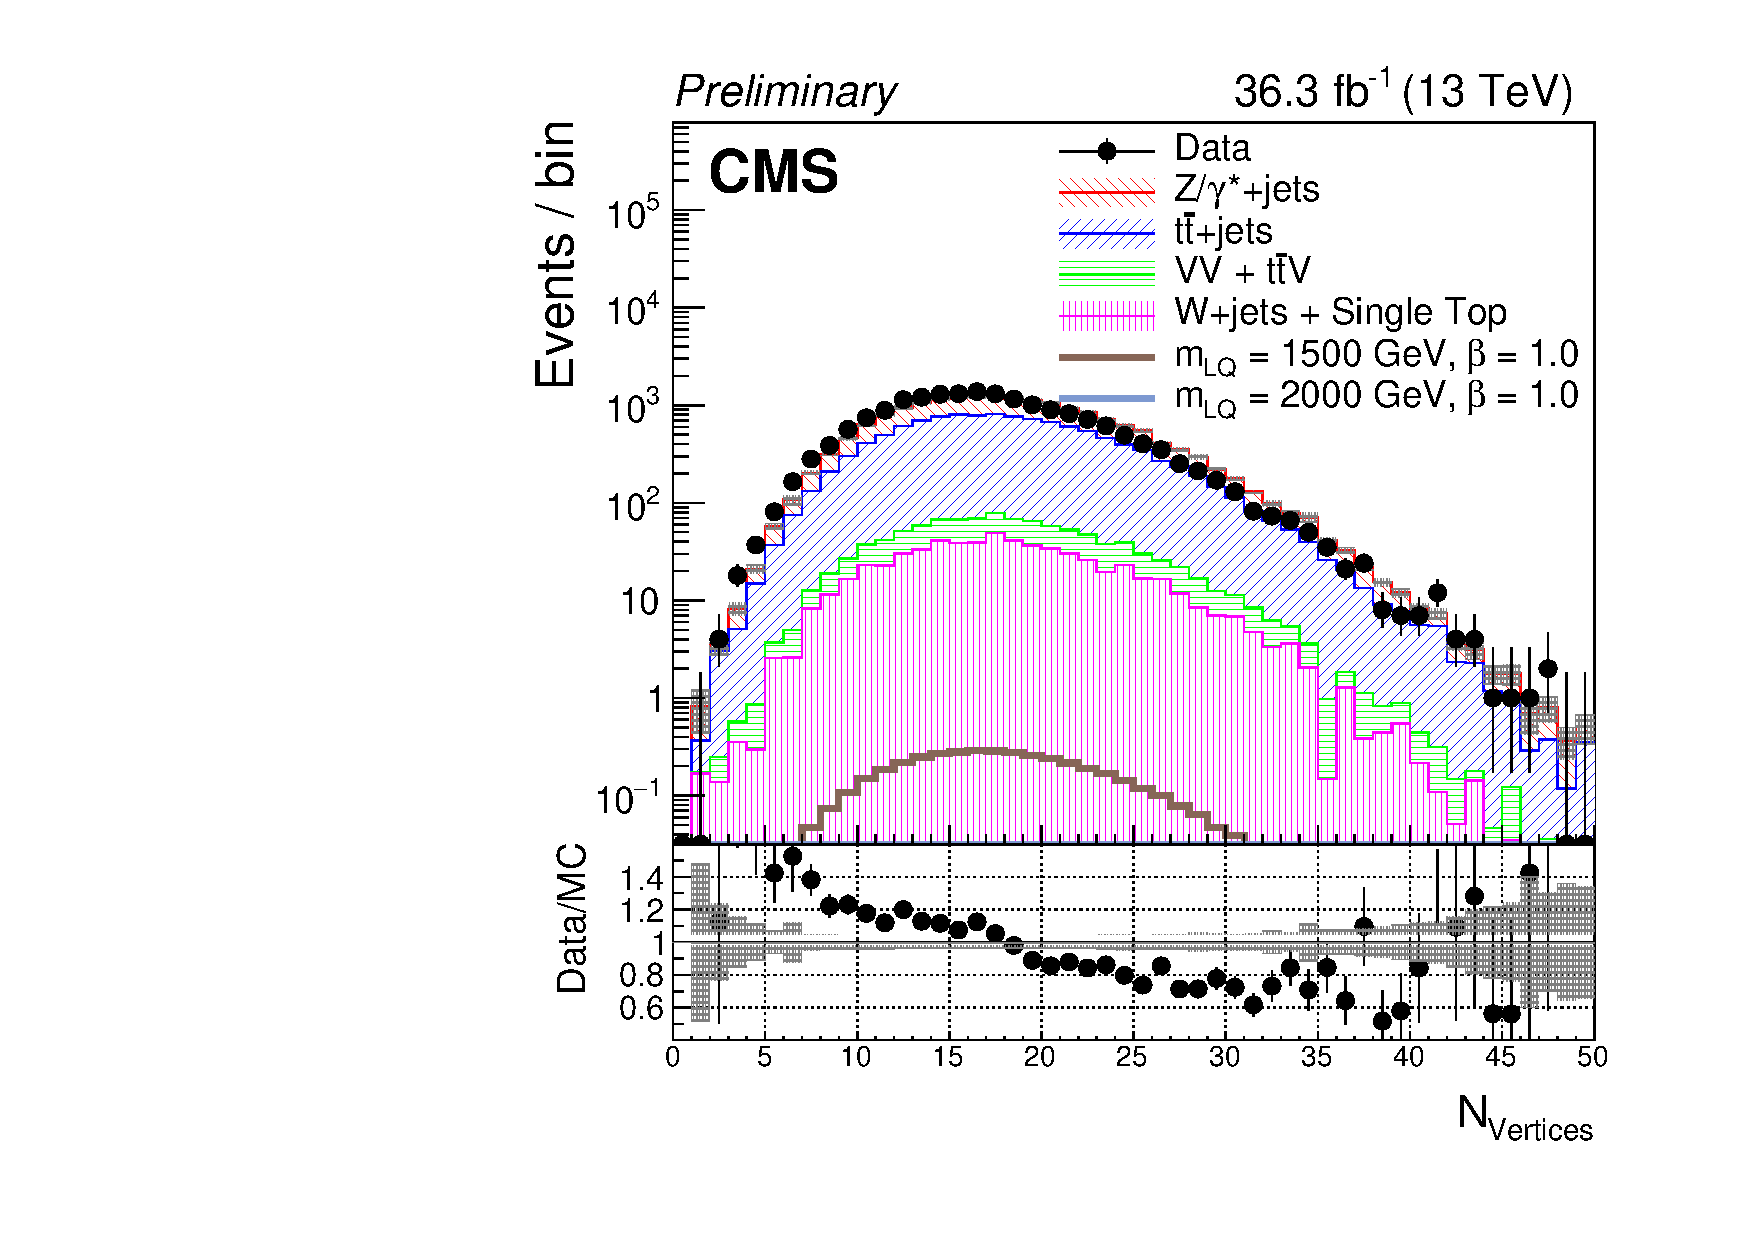
\includegraphics[width=.32\textwidth]{Images/Analysis/Results_2016_Unblinded/Plots/Preselection/BasicLQ_uujj_GoodVertexCount_standard.pdf}}
       {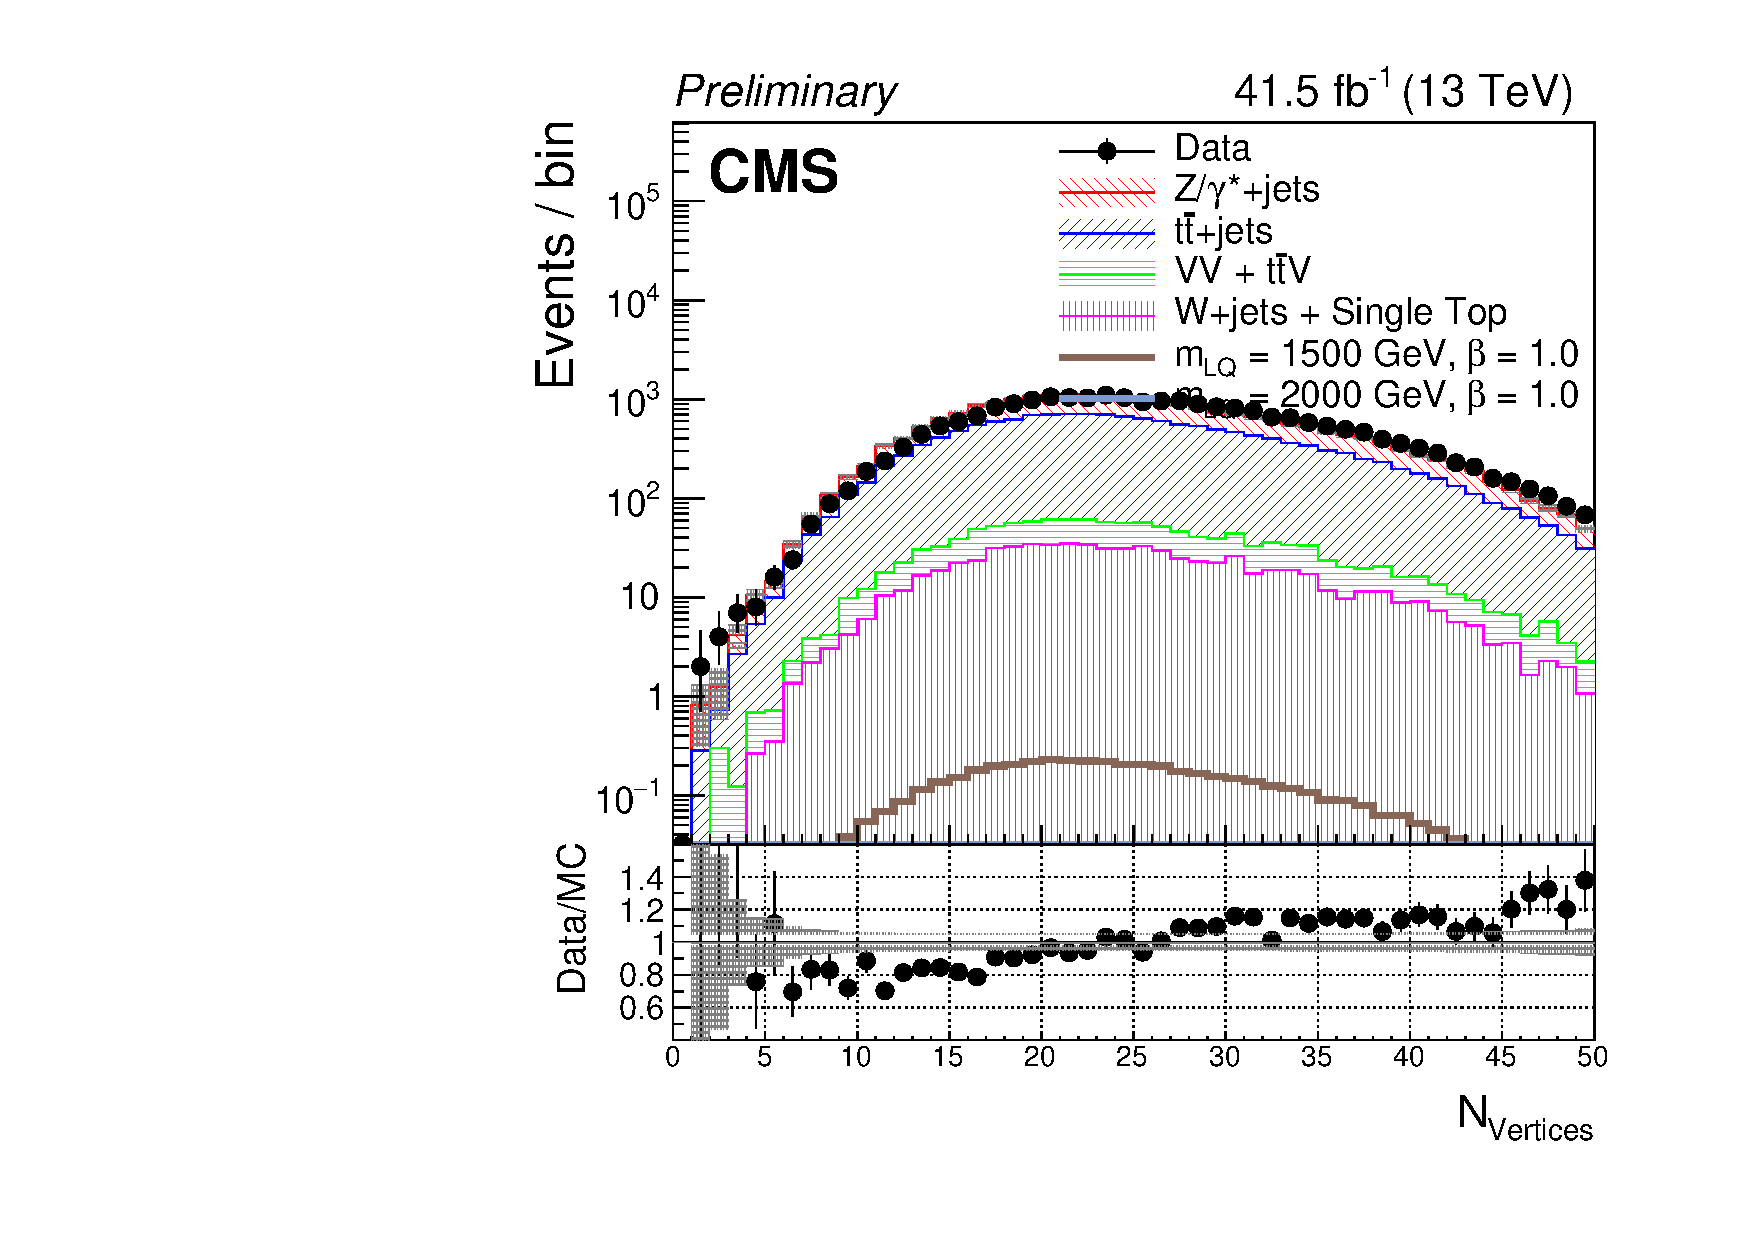
\includegraphics[width=.32\textwidth]{Images/Analysis/Results_2017_Unblinded/Plots/Preselection/BasicLQ_uujj_GoodVertexCount_standard.pdf}}
       {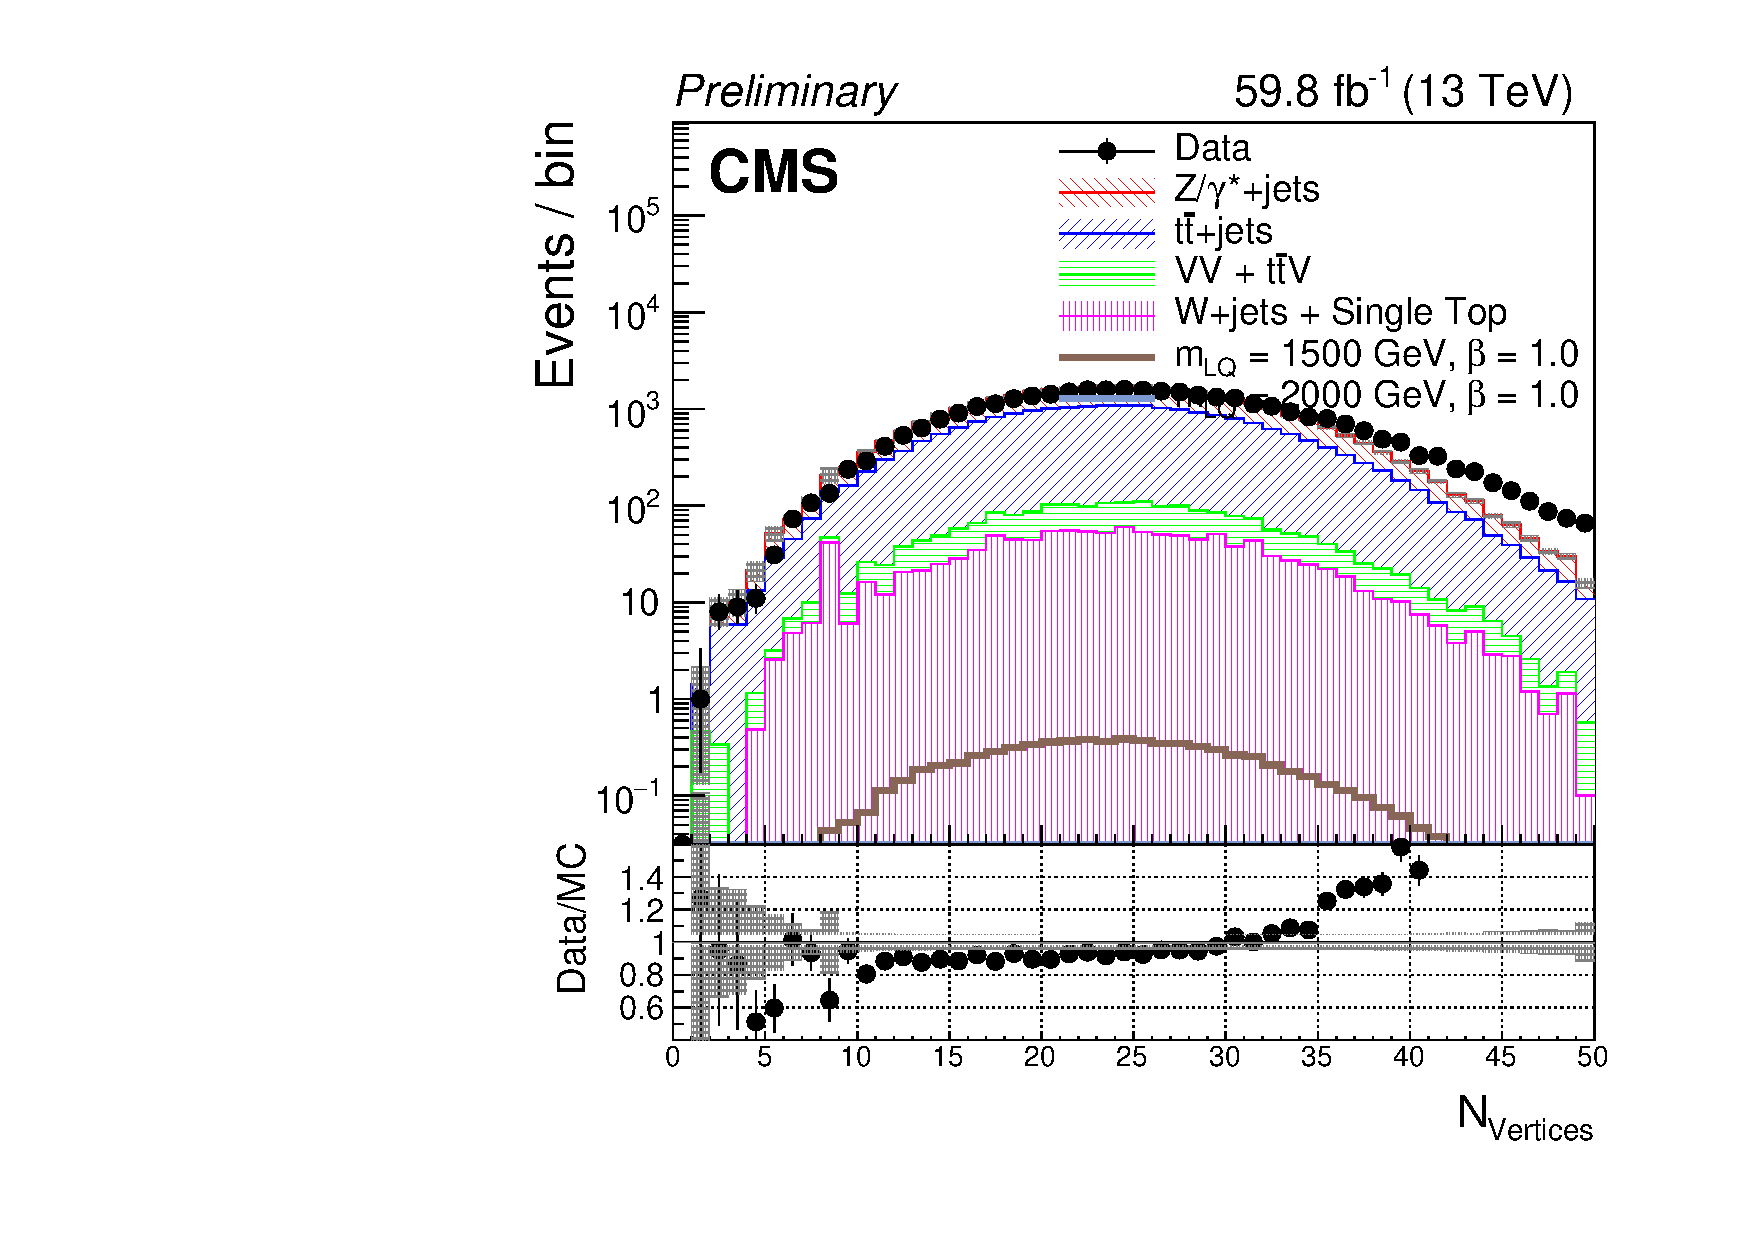
\includegraphics[width=.32\textwidth]{Images/Analysis/Results_2018_Unblinded/Plots/Preselection/BasicLQ_uujj_GoodVertexCount_standard.pdf}}
       \caption{A comparison of the number of reconstructed vertices at preselection level in 2016 (left), 2017 (middle) and 2018 (right) data. Error bars shown represent statistical uncertainties, and systematic uncertainties are shown by gray hashing.}
       \label{figapp:vertex}
\end{figure}
\begin{figure}[H]
       \centering
       {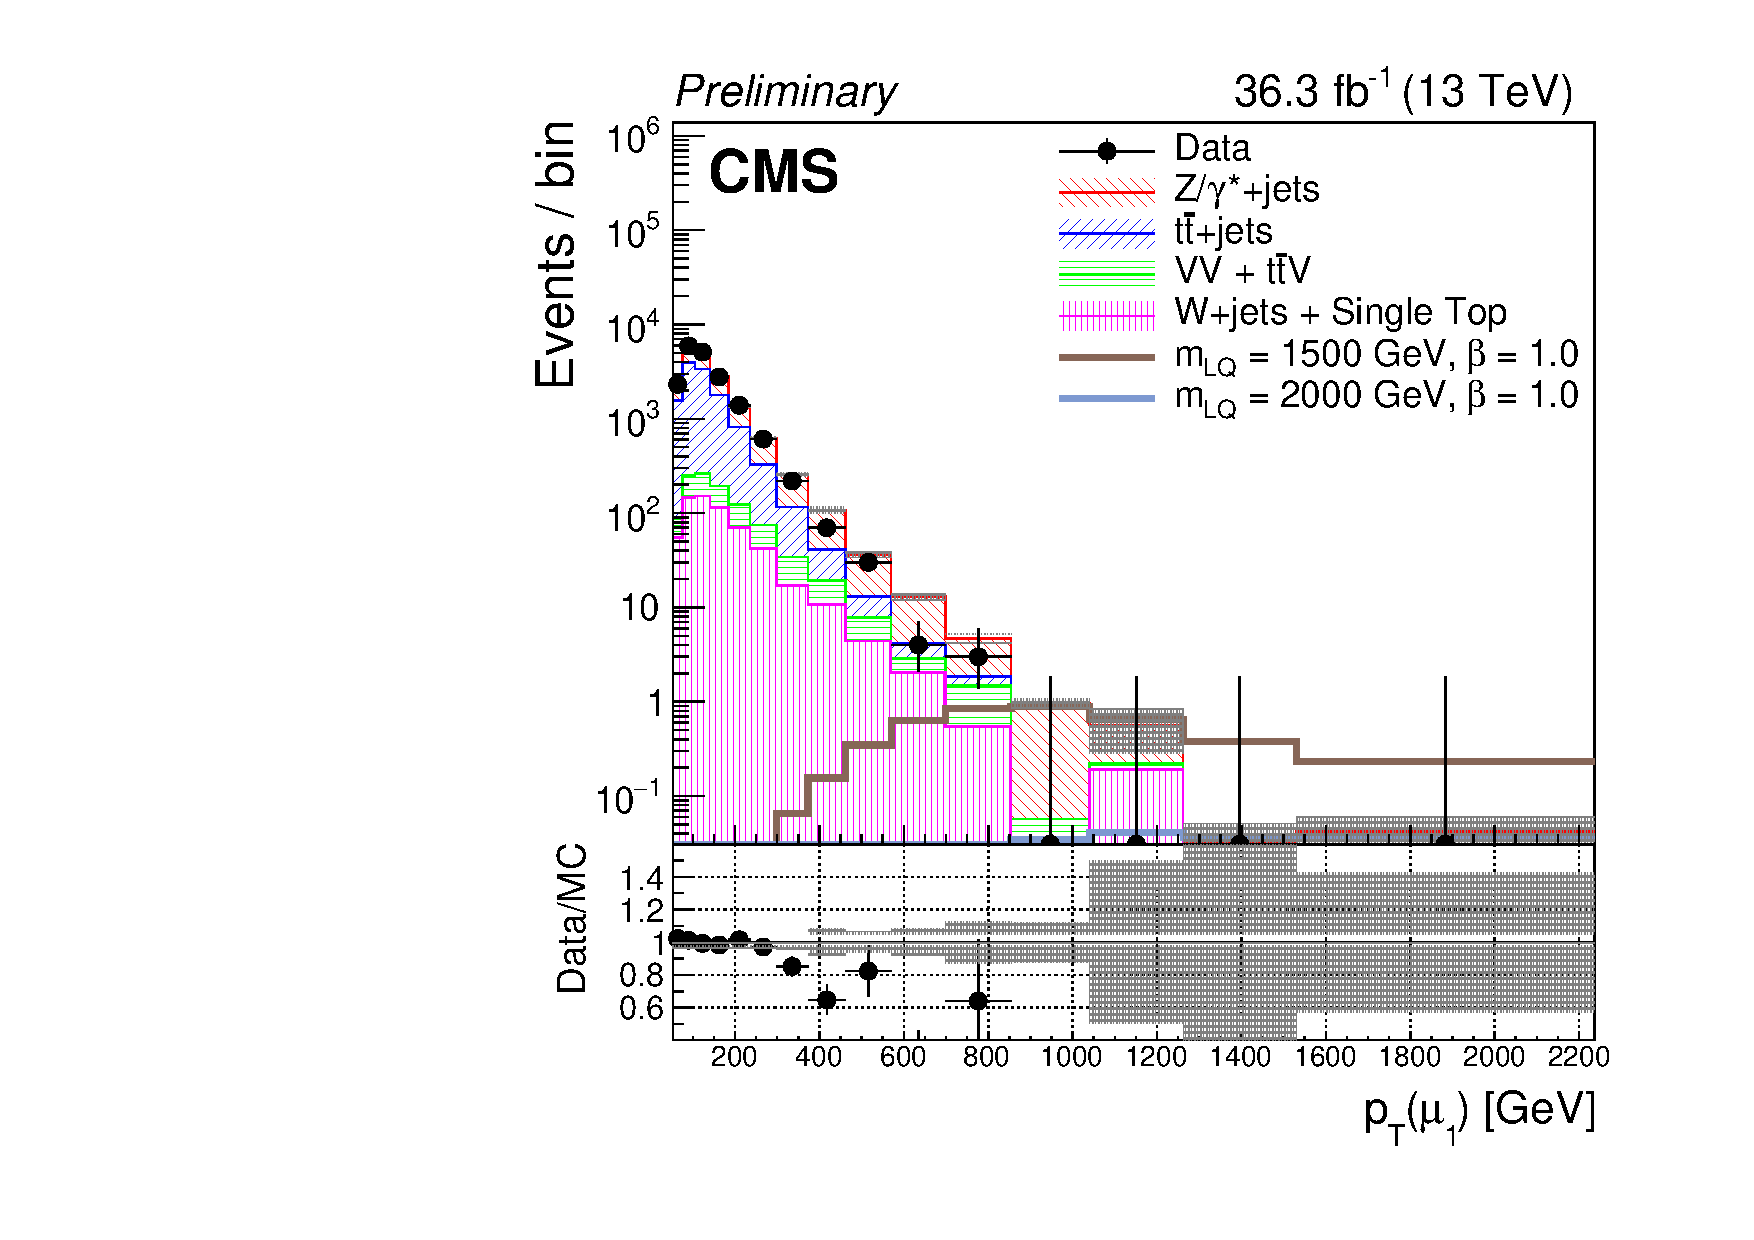
\includegraphics[width=.32\textwidth]{Images/Analysis/Results_2016_Unblinded/Plots/Preselection/BasicLQ_uujj_Pt_muon1_standard.pdf}}
       {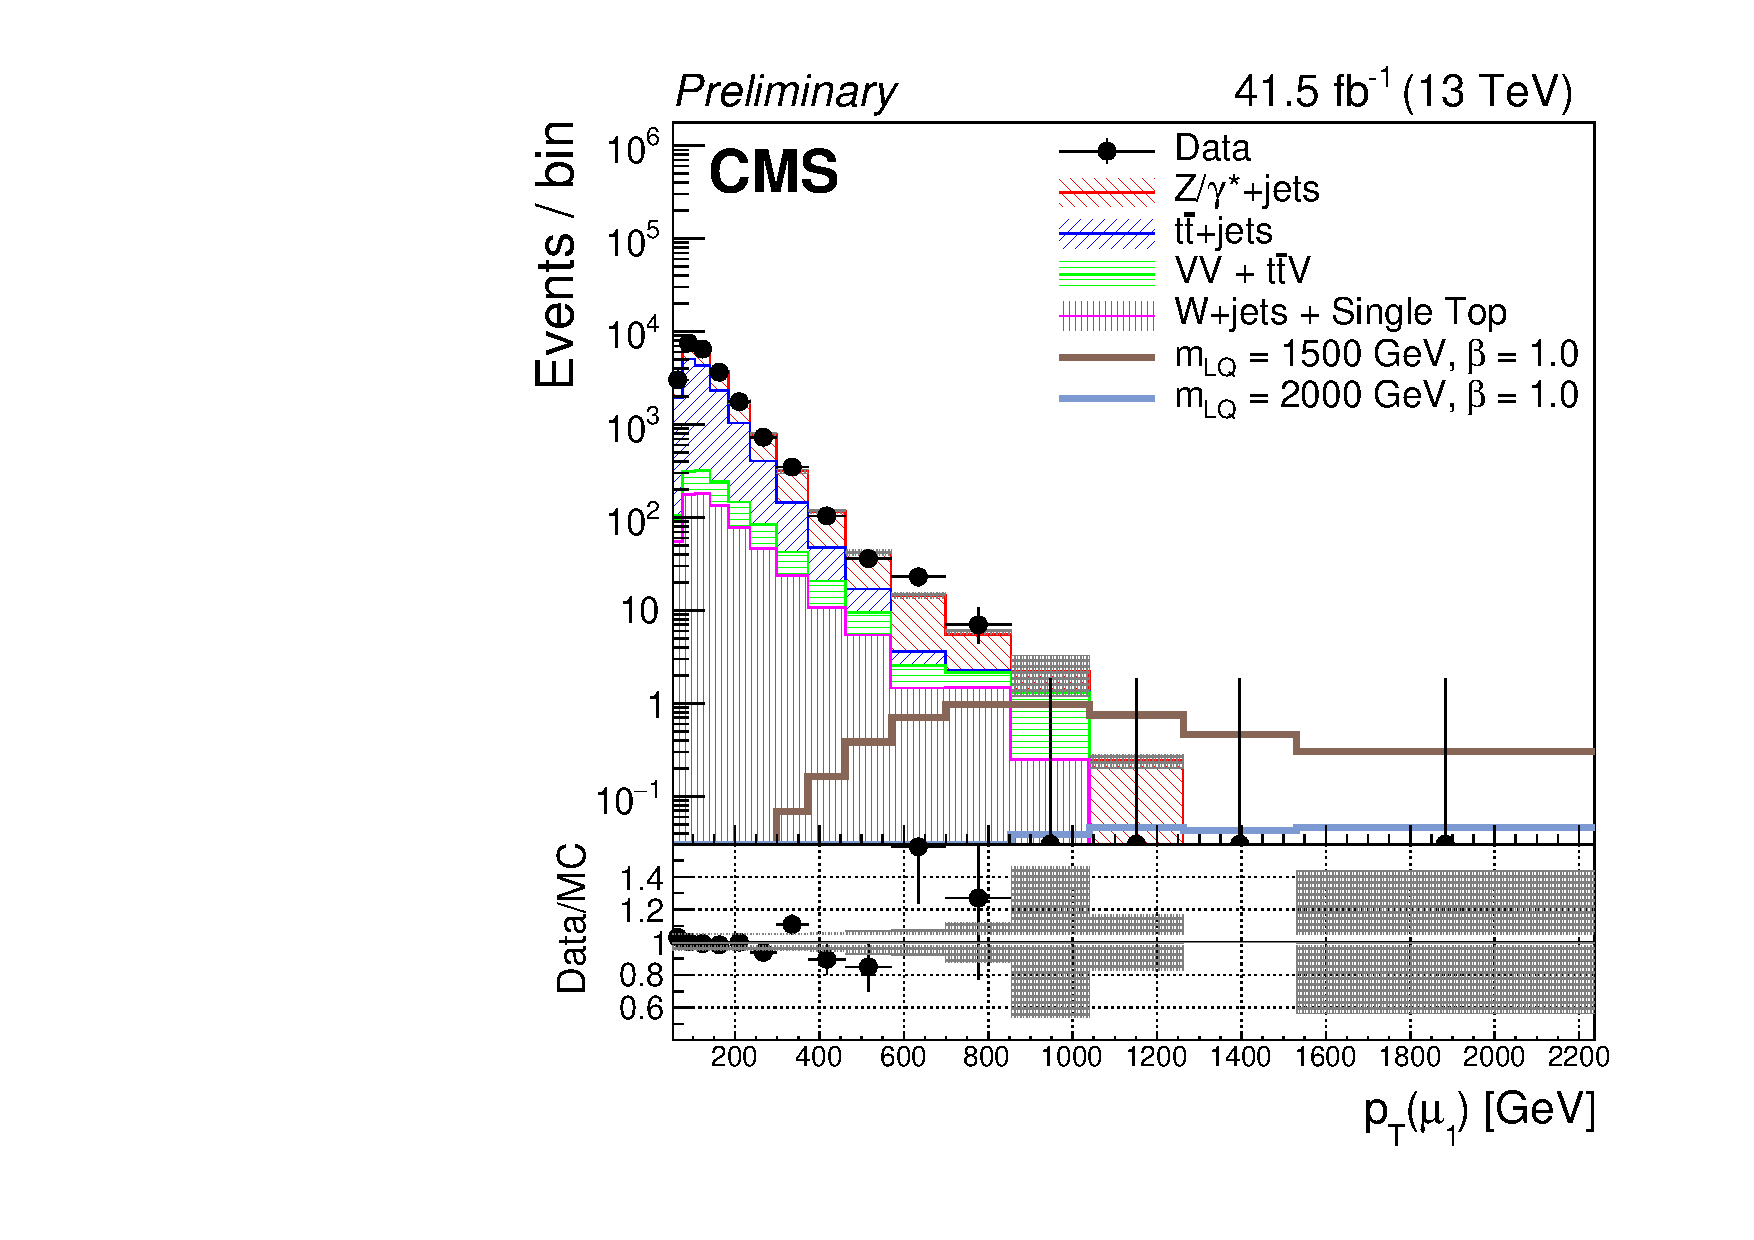
\includegraphics[width=.32\textwidth]{Images/Analysis/Results_2017_Unblinded/Plots/Preselection/BasicLQ_uujj_Pt_muon1_standard.pdf}}
       {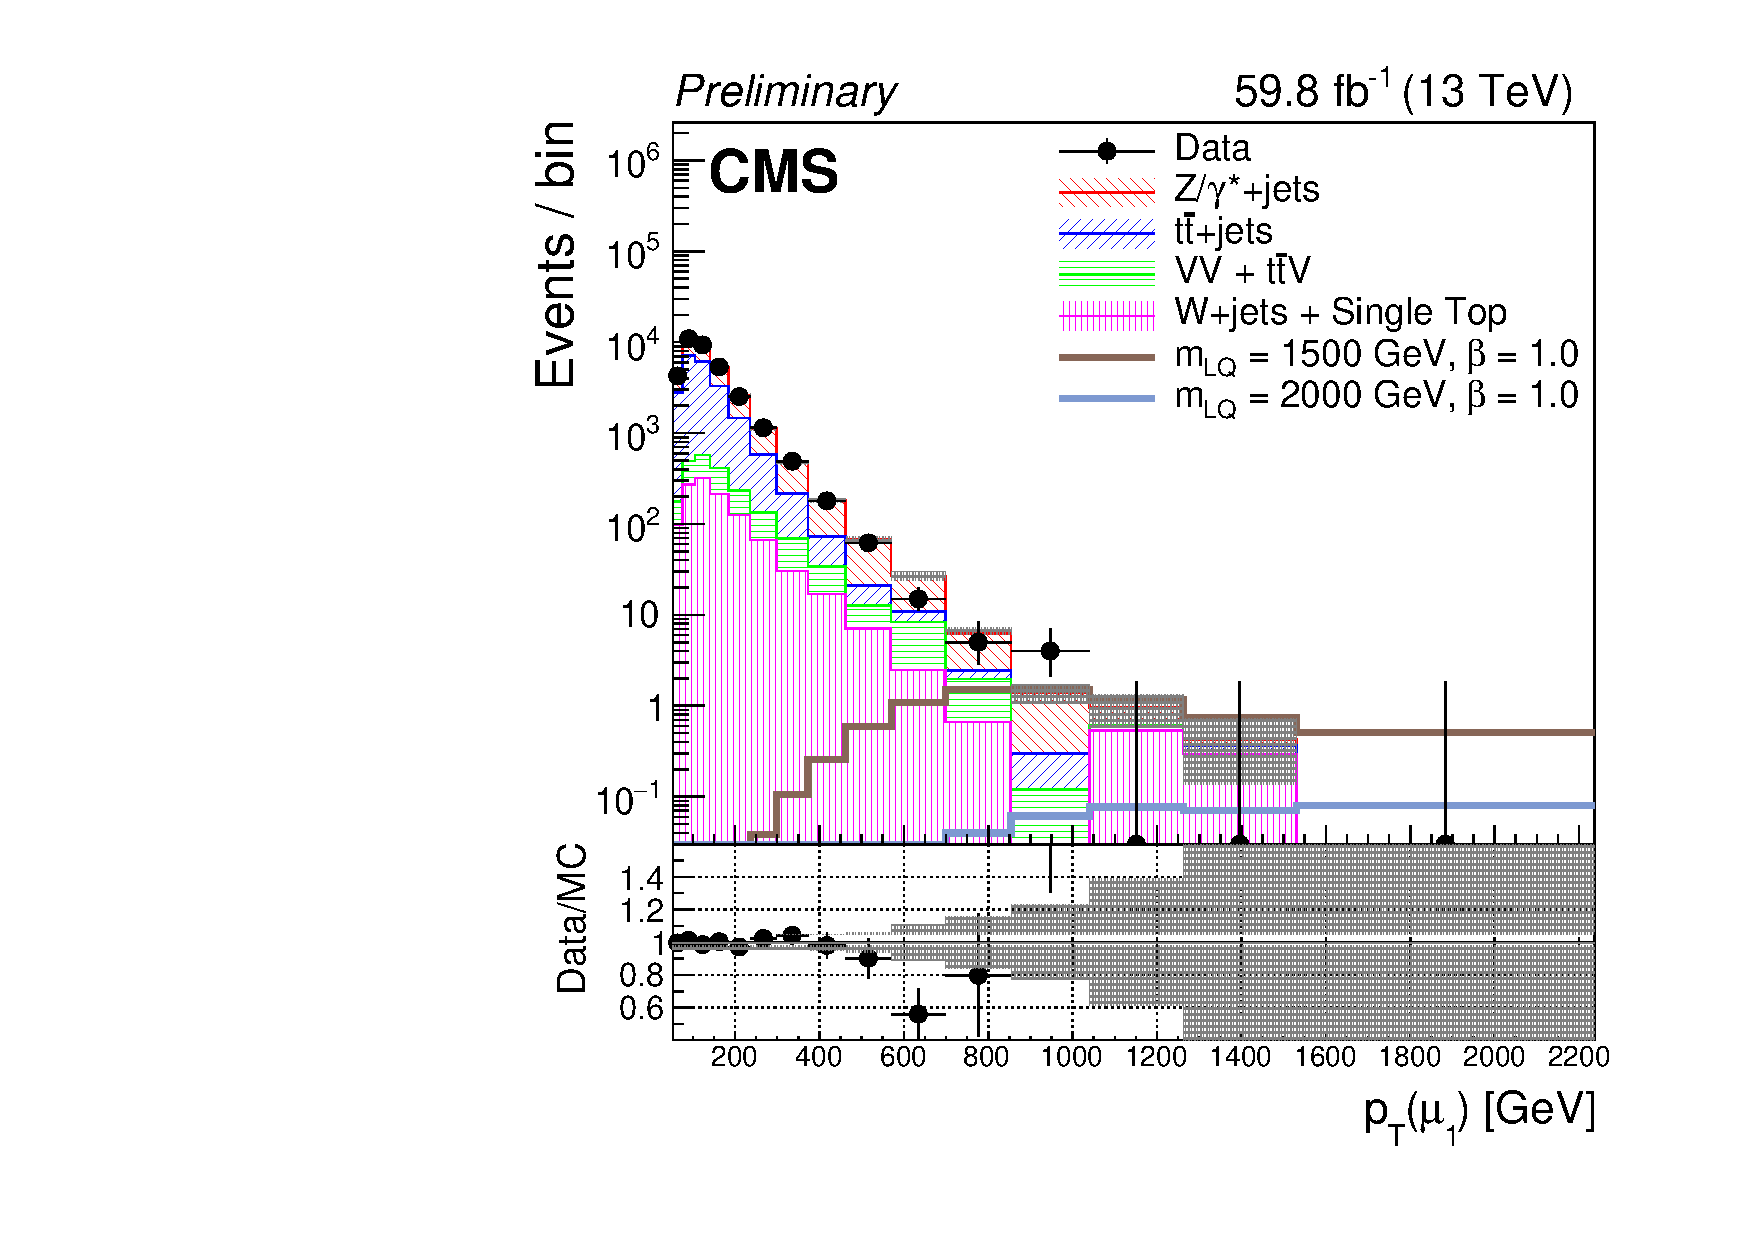
\includegraphics[width=.32\textwidth]{Images/Analysis/Results_2018_Unblinded/Plots/Preselection/BasicLQ_uujj_Pt_muon1_standard.pdf}}
       {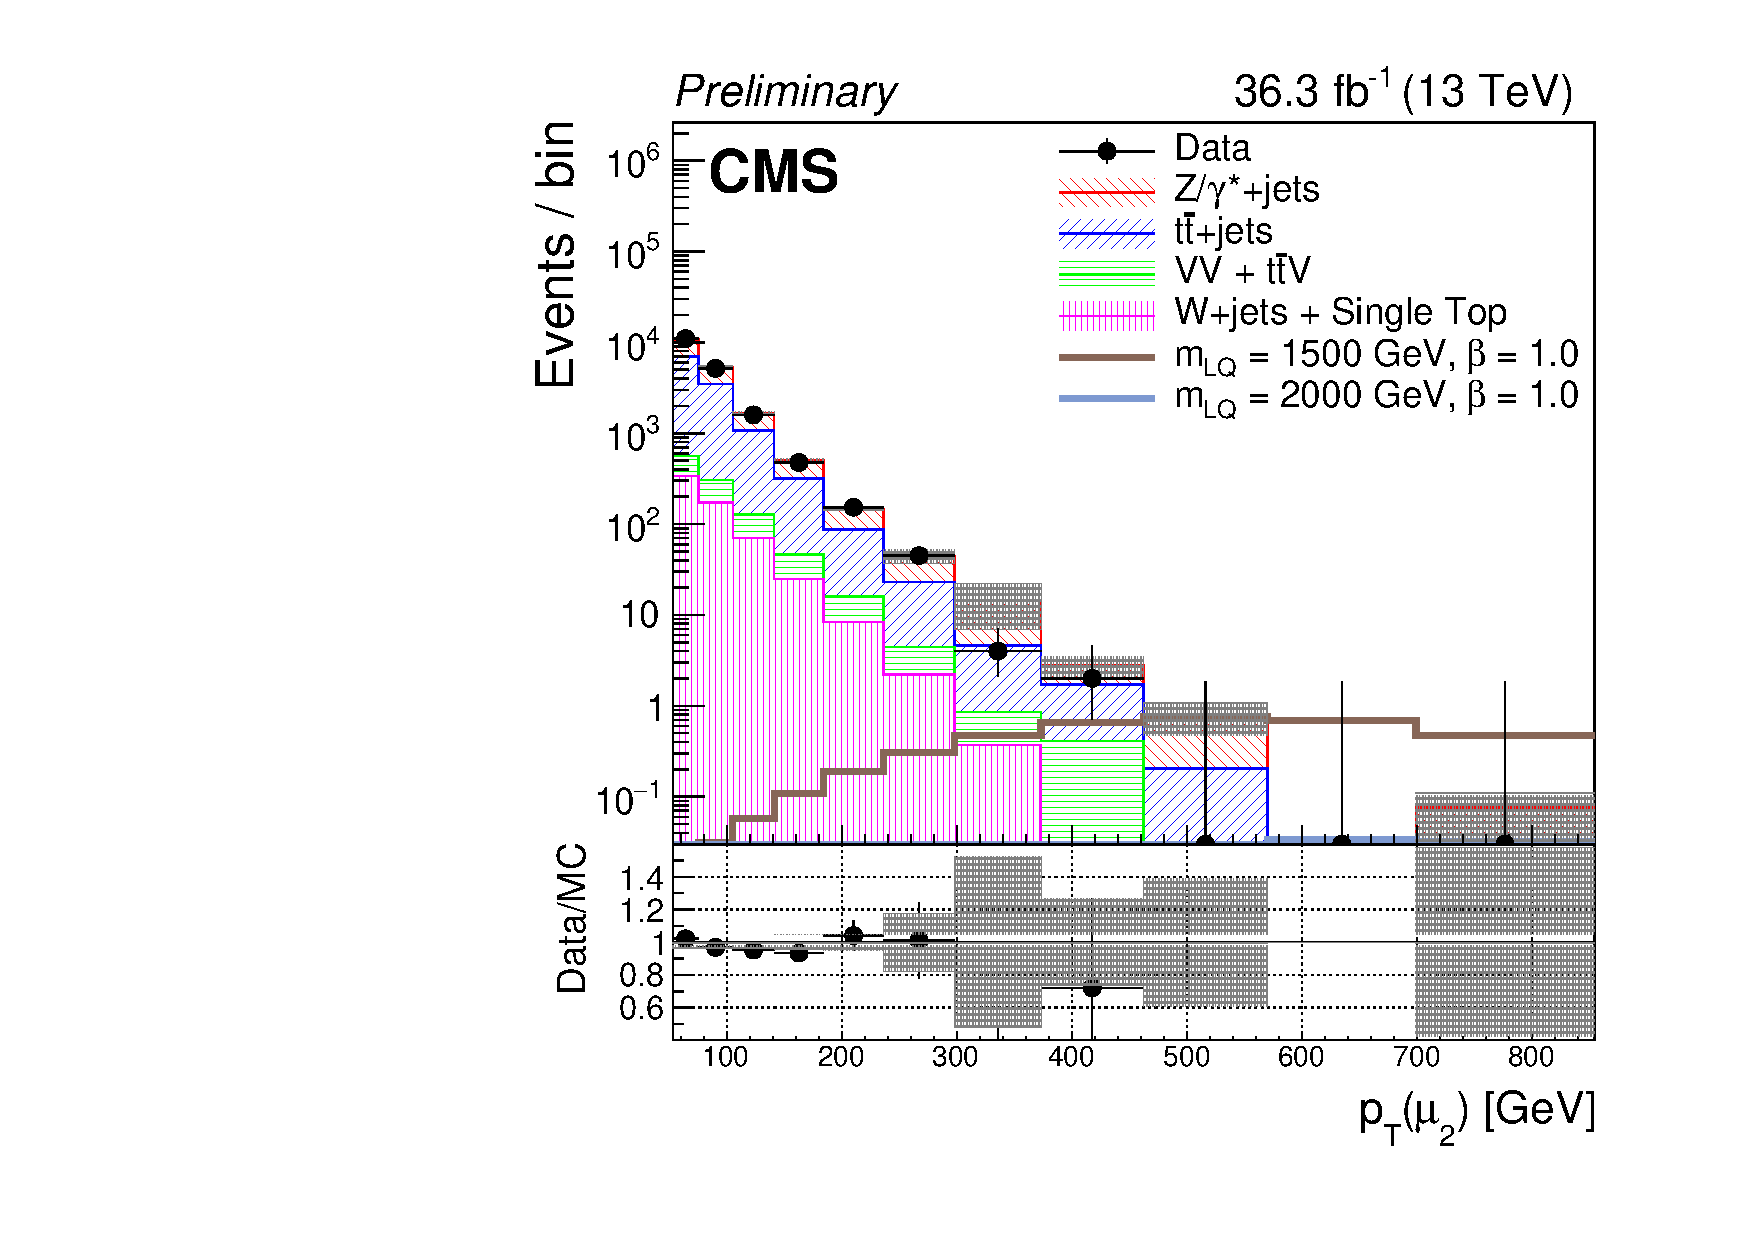
\includegraphics[width=.32\textwidth]{Images/Analysis/Results_2016_Unblinded/Plots/Preselection/BasicLQ_uujj_Pt_muon2_standard.pdf}}
       {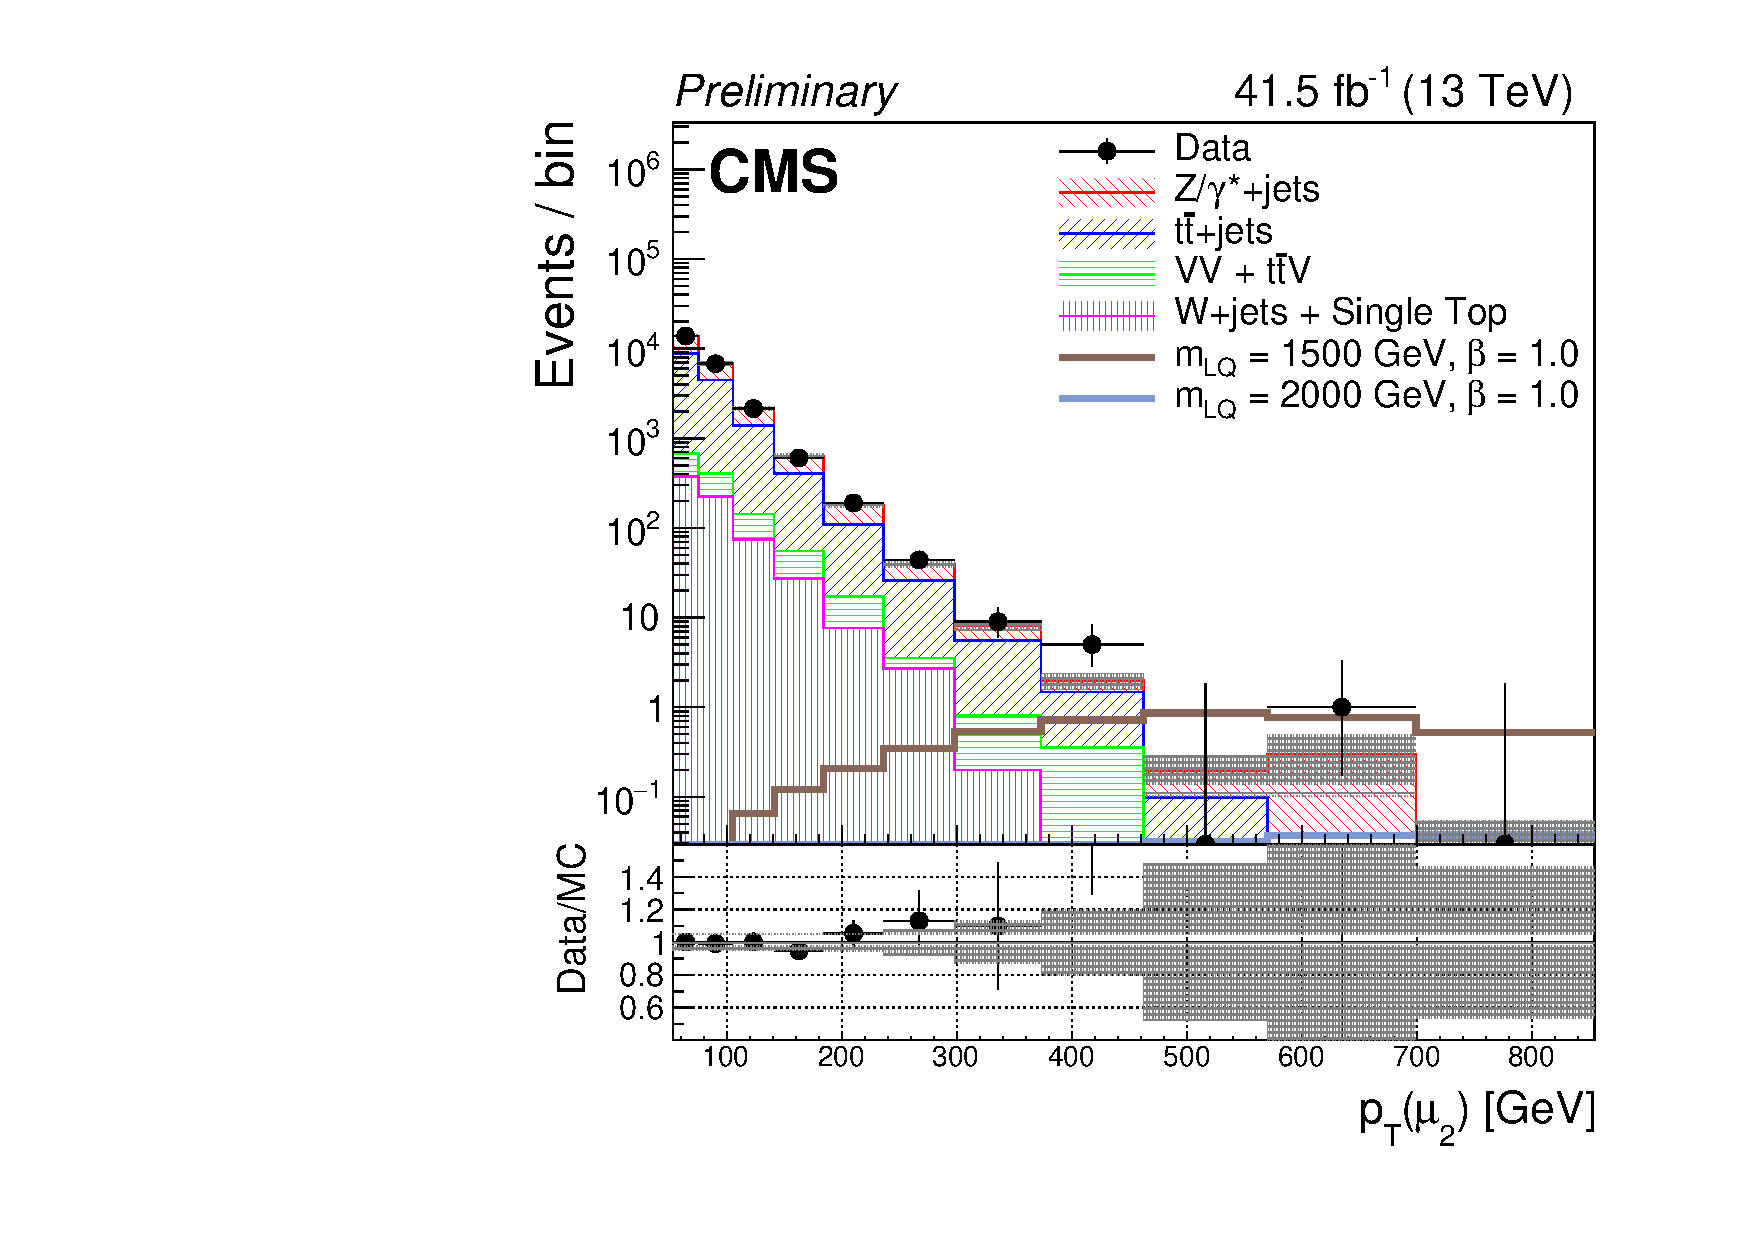
\includegraphics[width=.32\textwidth]{Images/Analysis/Results_2017_Unblinded/Plots/Preselection/BasicLQ_uujj_Pt_muon2_standard.pdf}}
       {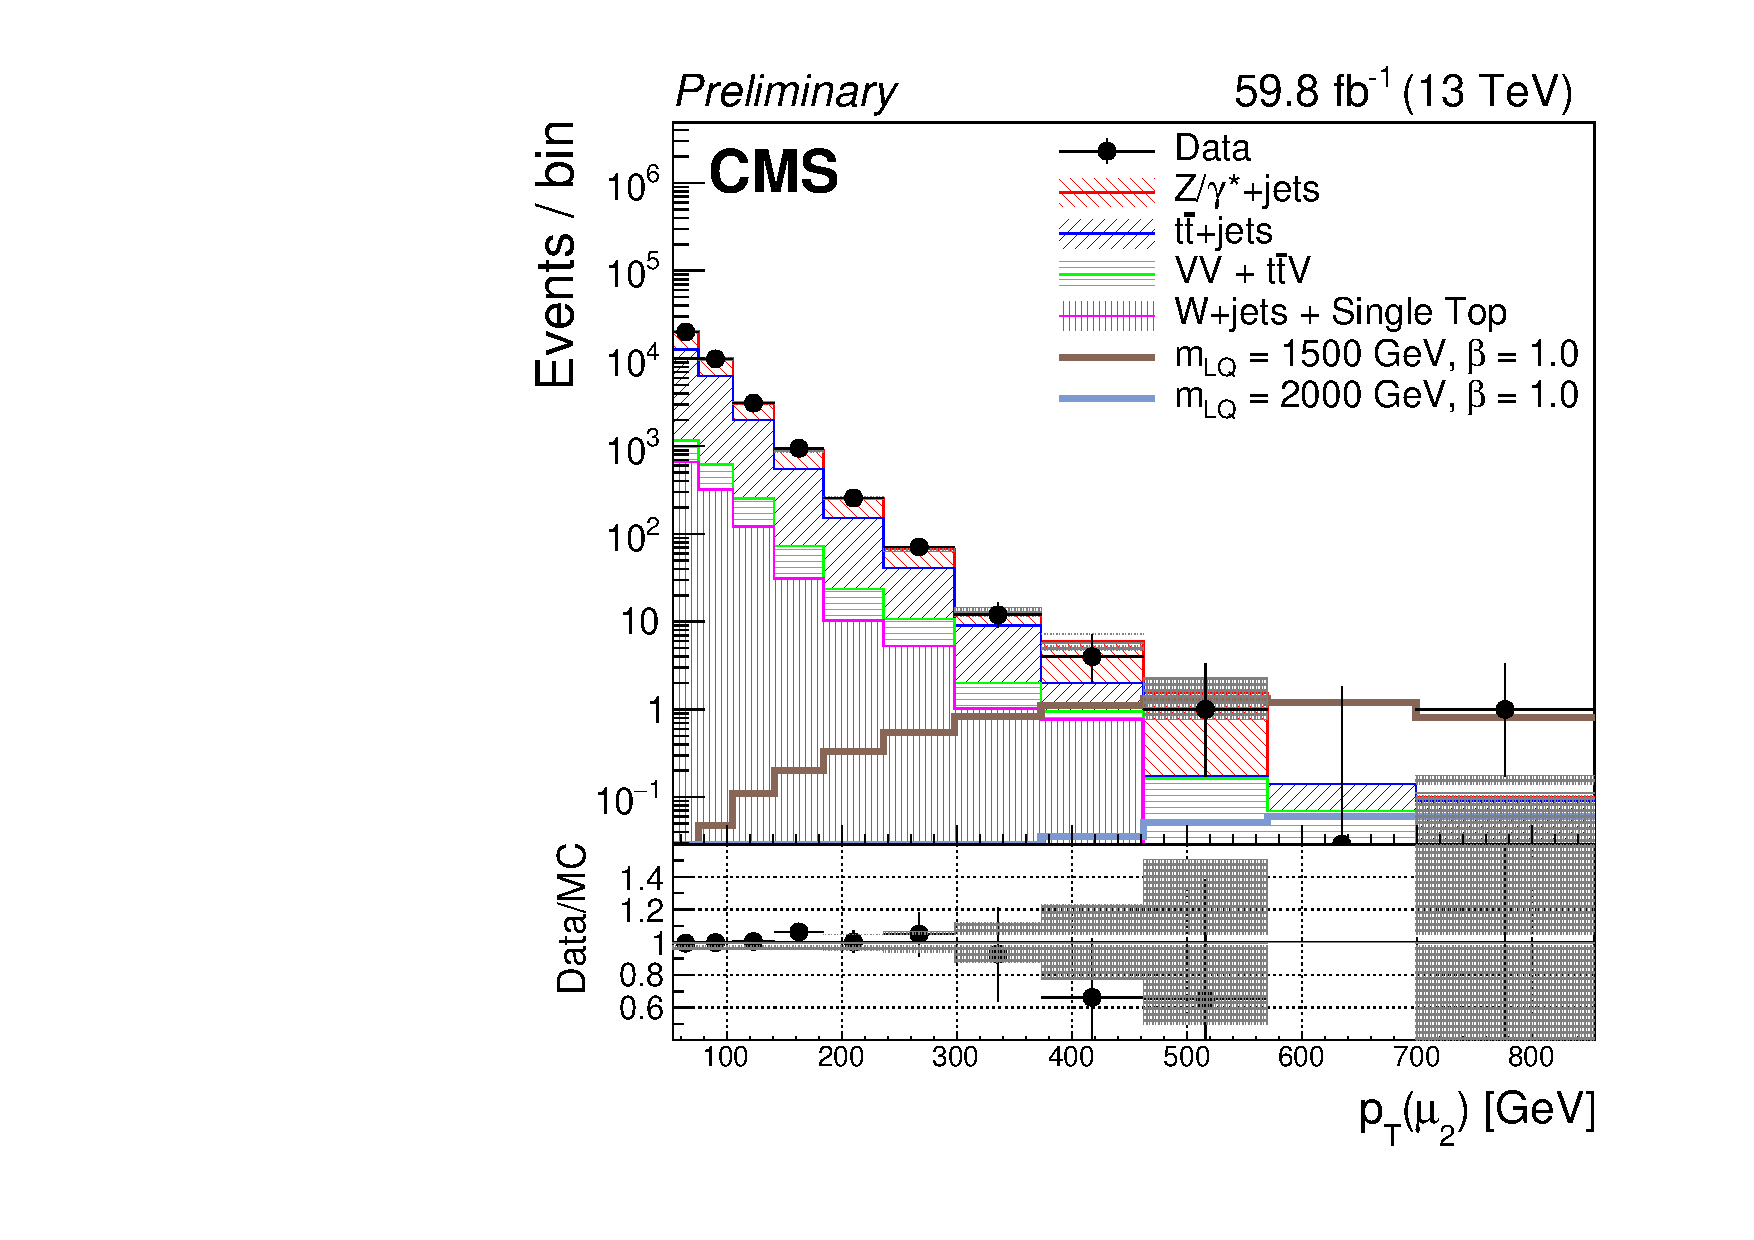
\includegraphics[width=.32\textwidth]{Images/Analysis/Results_2018_Unblinded/Plots/Preselection/BasicLQ_uujj_Pt_muon2_standard.pdf}}
       {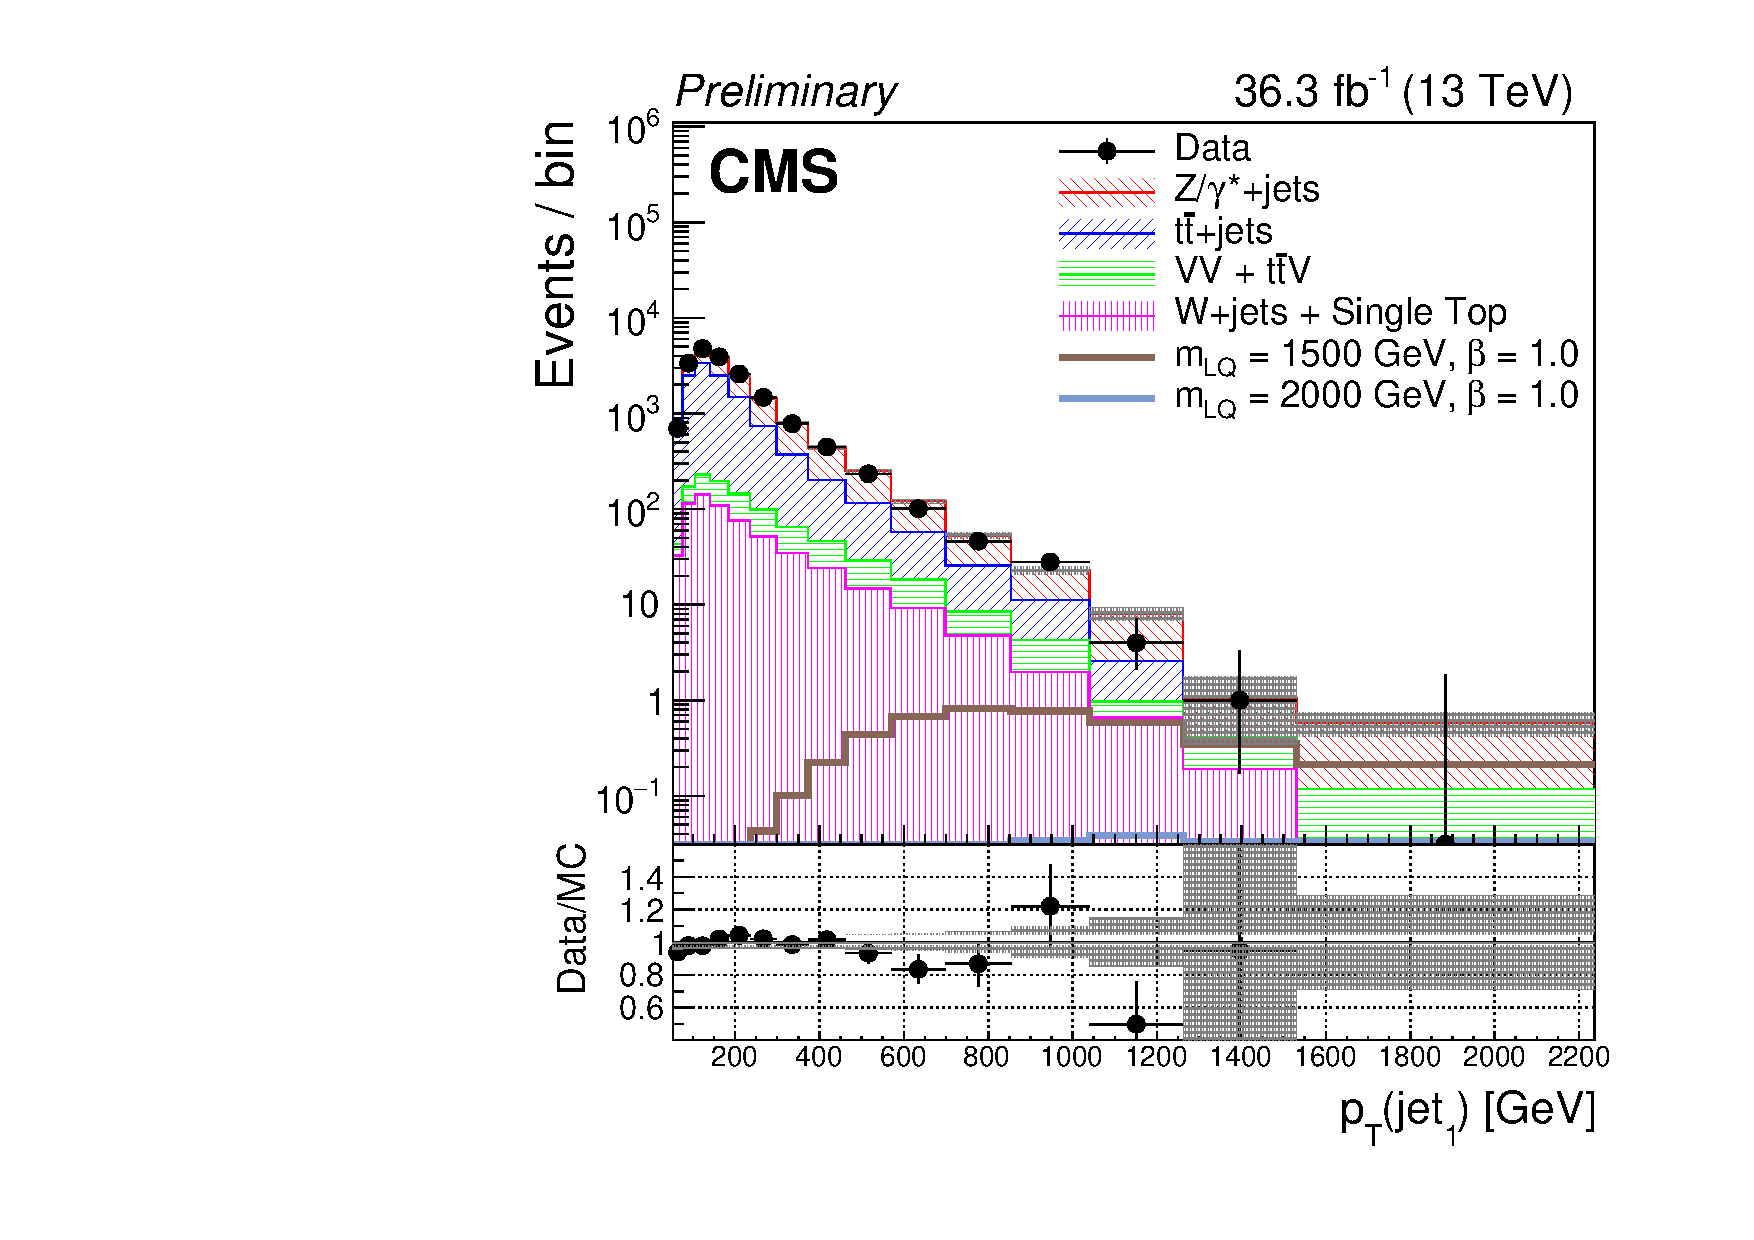
\includegraphics[width=.32\textwidth]{Images/Analysis/Results_2016_Unblinded/Plots/Preselection/BasicLQ_uujj_Pt_jet1_standard.pdf}}
       {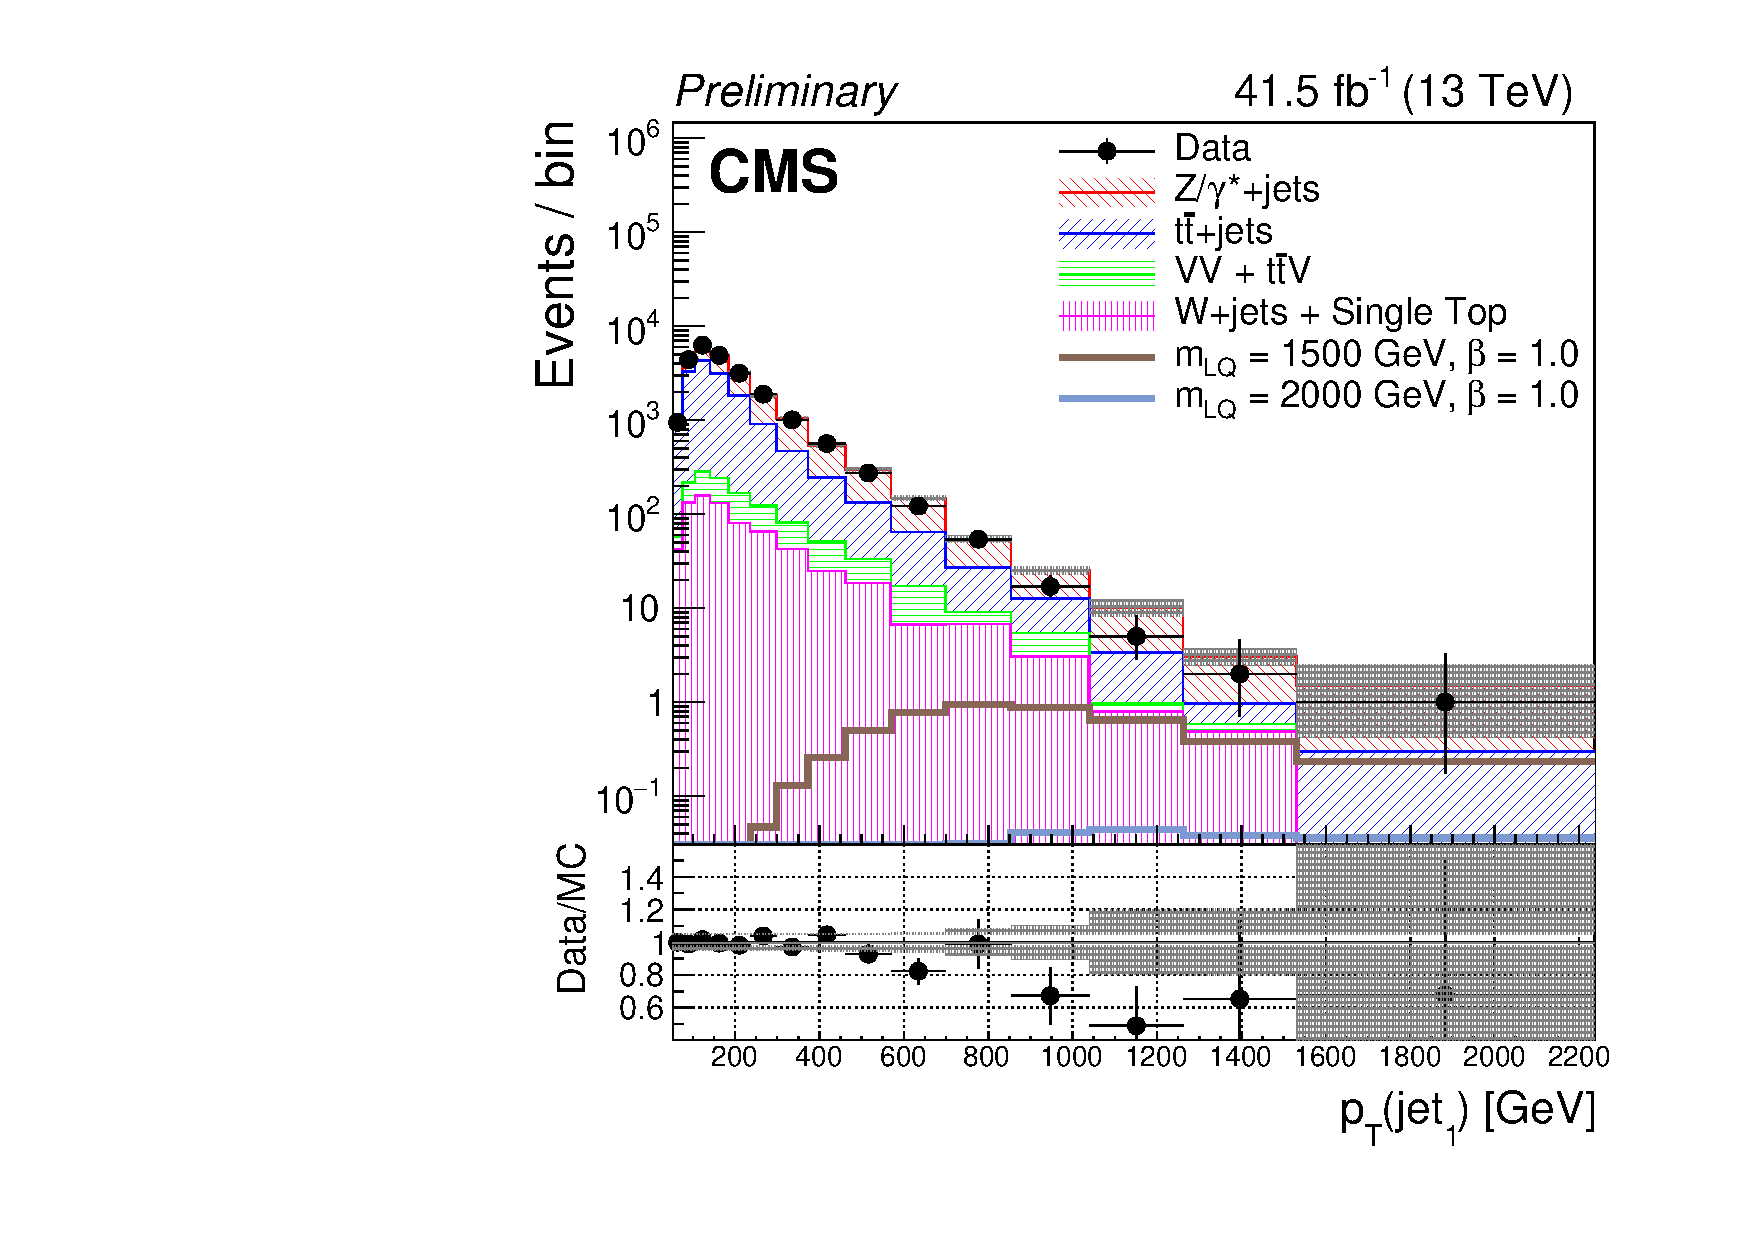
\includegraphics[width=.32\textwidth]{Images/Analysis/Results_2017_Unblinded/Plots/Preselection/BasicLQ_uujj_Pt_jet1_standard.pdf}}
       {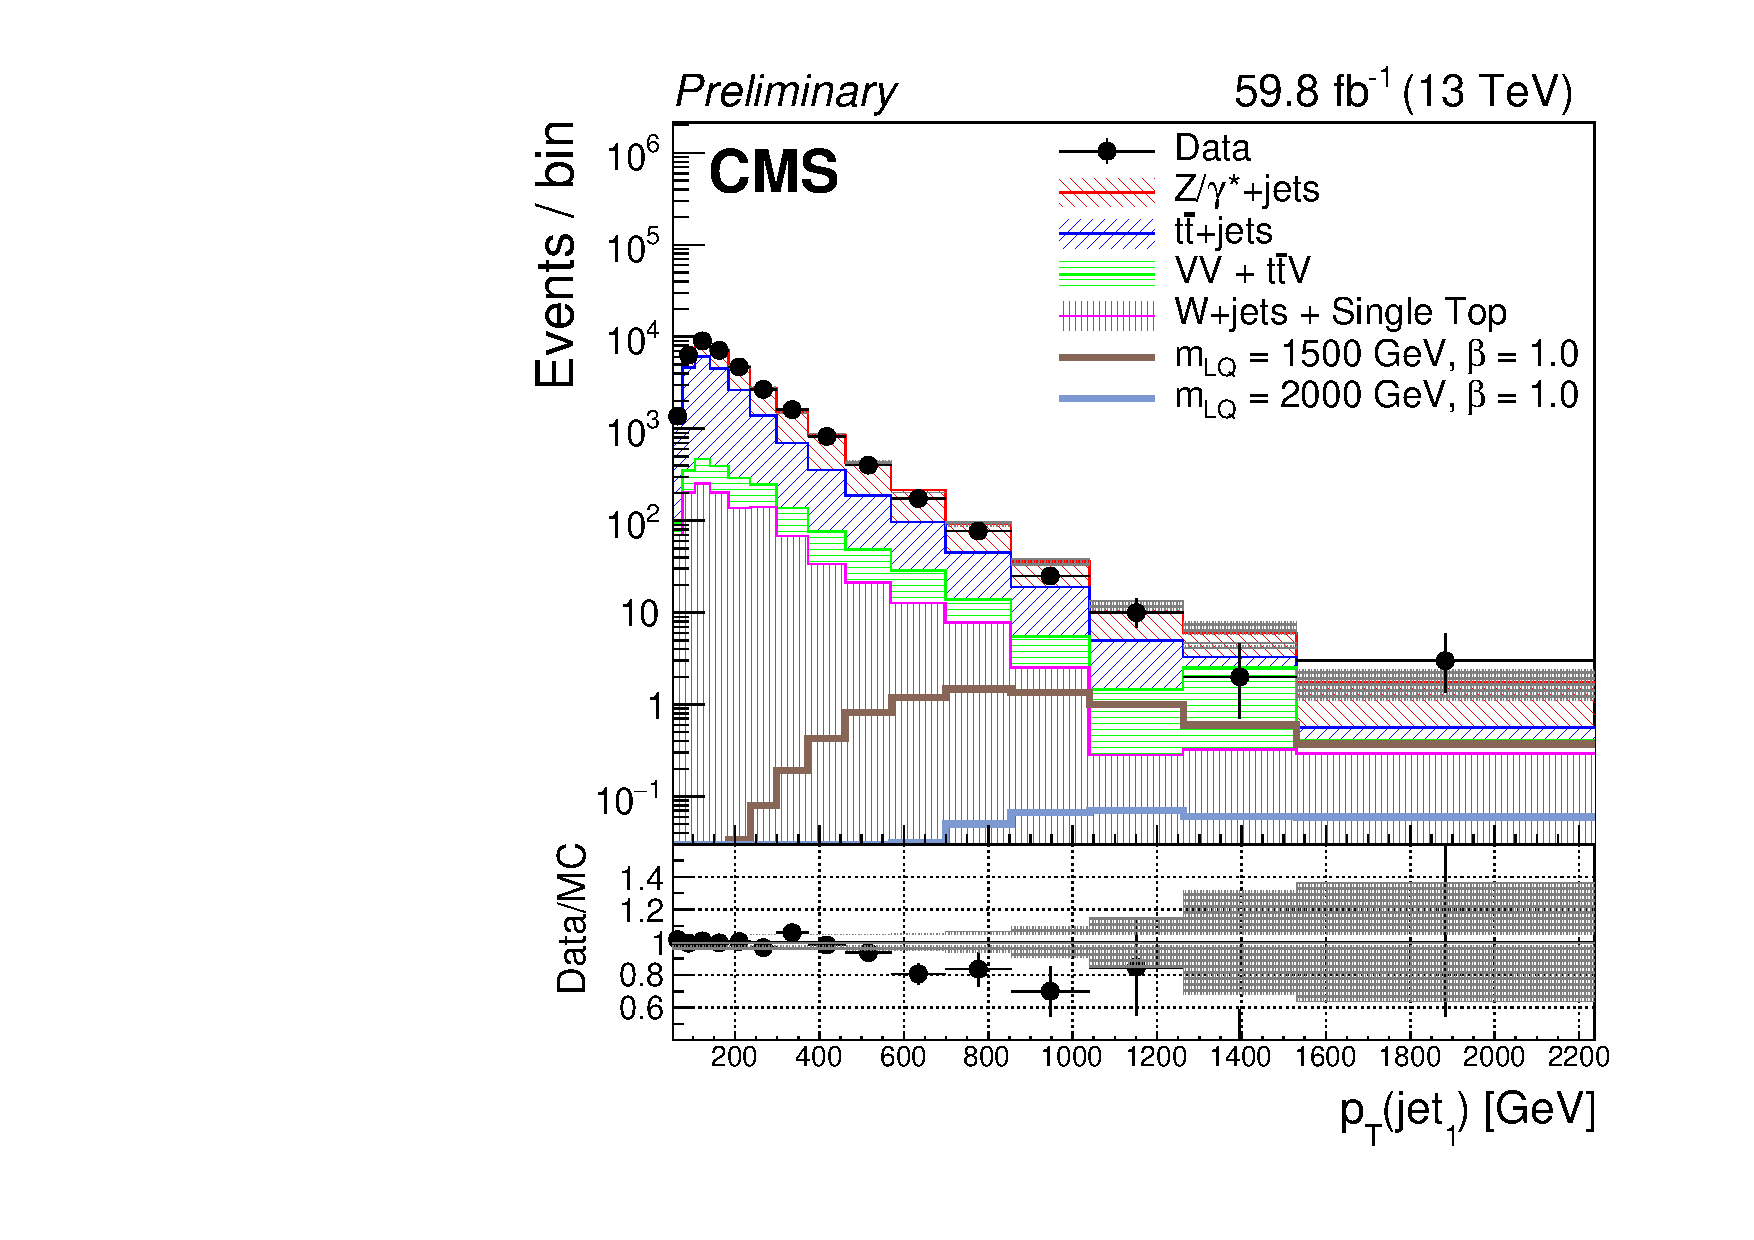
\includegraphics[width=.32\textwidth]{Images/Analysis/Results_2018_Unblinded/Plots/Preselection/BasicLQ_uujj_Pt_jet1_standard.pdf}}
       {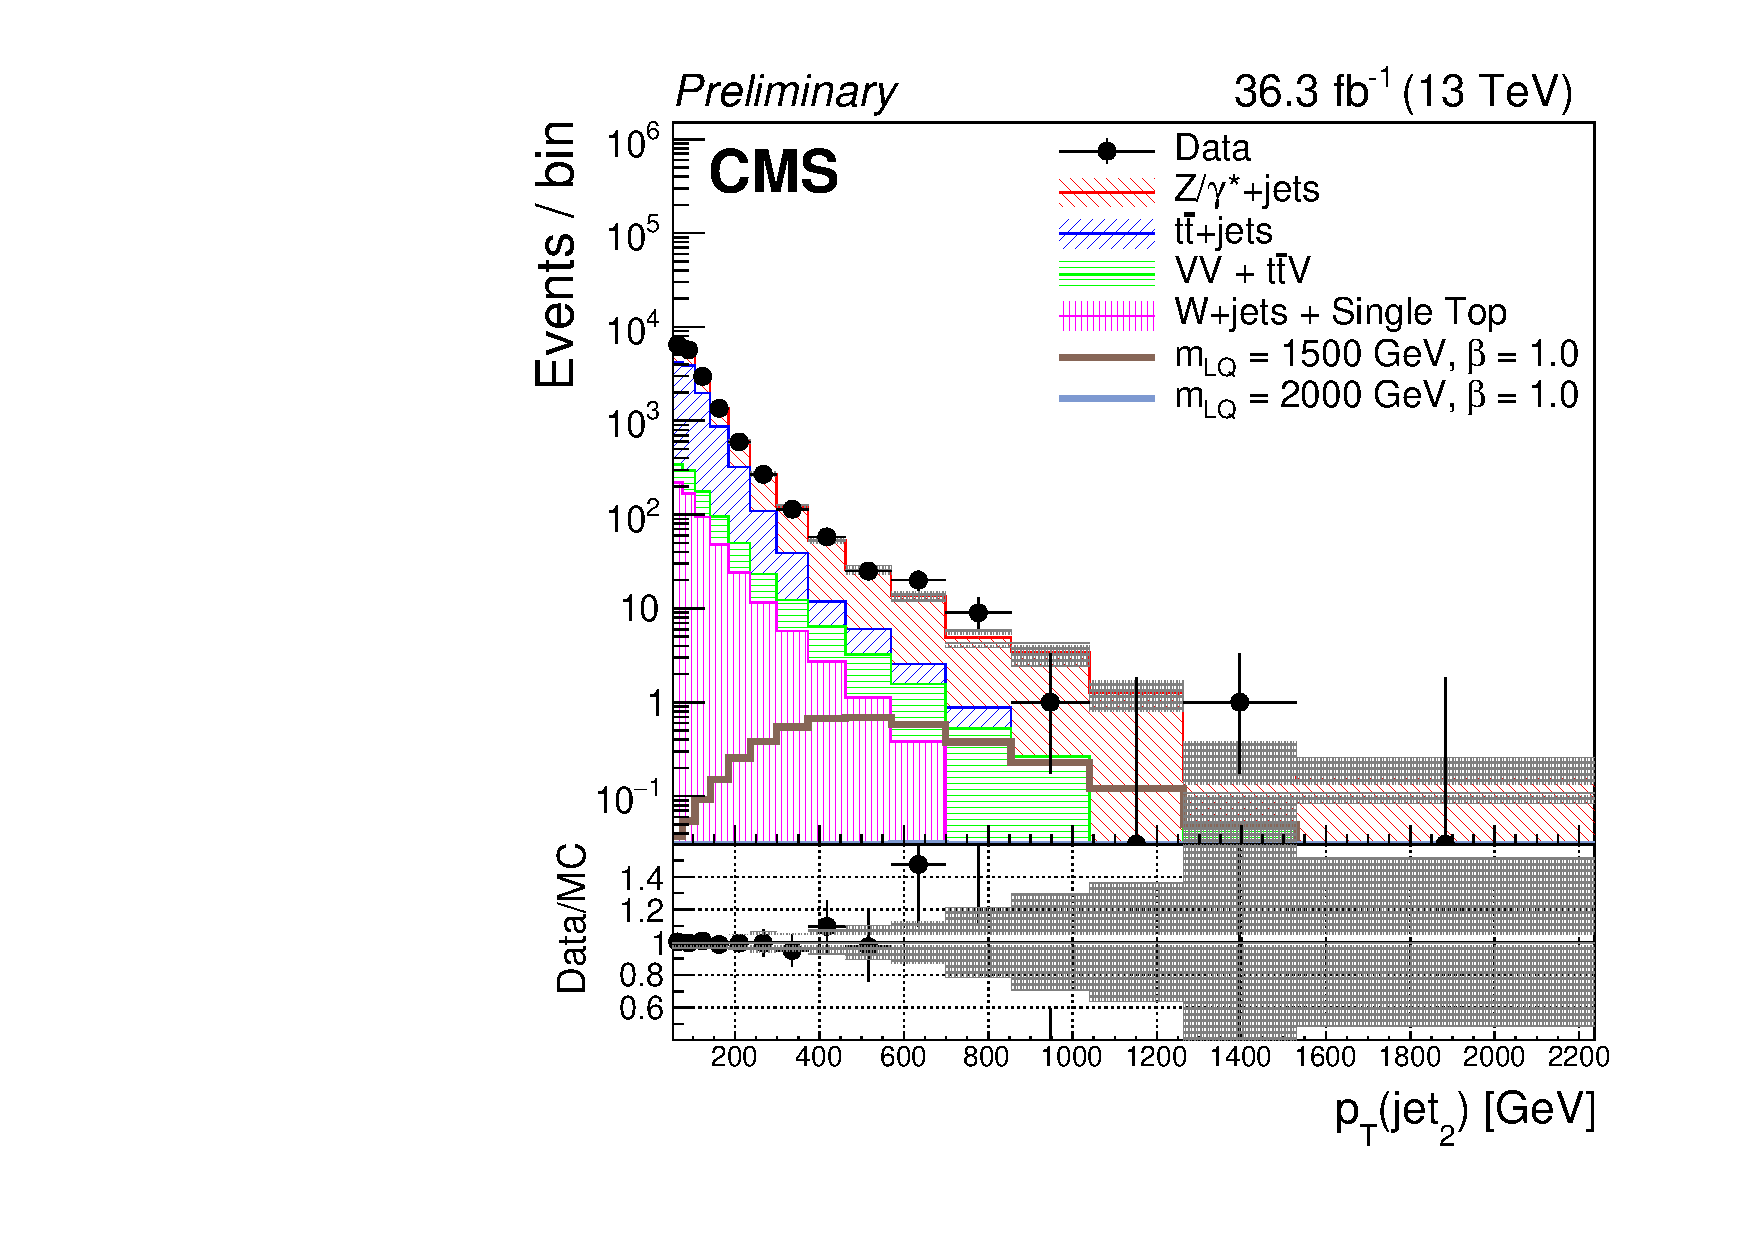
\includegraphics[width=.32\textwidth]{Images/Analysis/Results_2016_Unblinded/Plots/Preselection/BasicLQ_uujj_Pt_jet2_standard.pdf}}
       {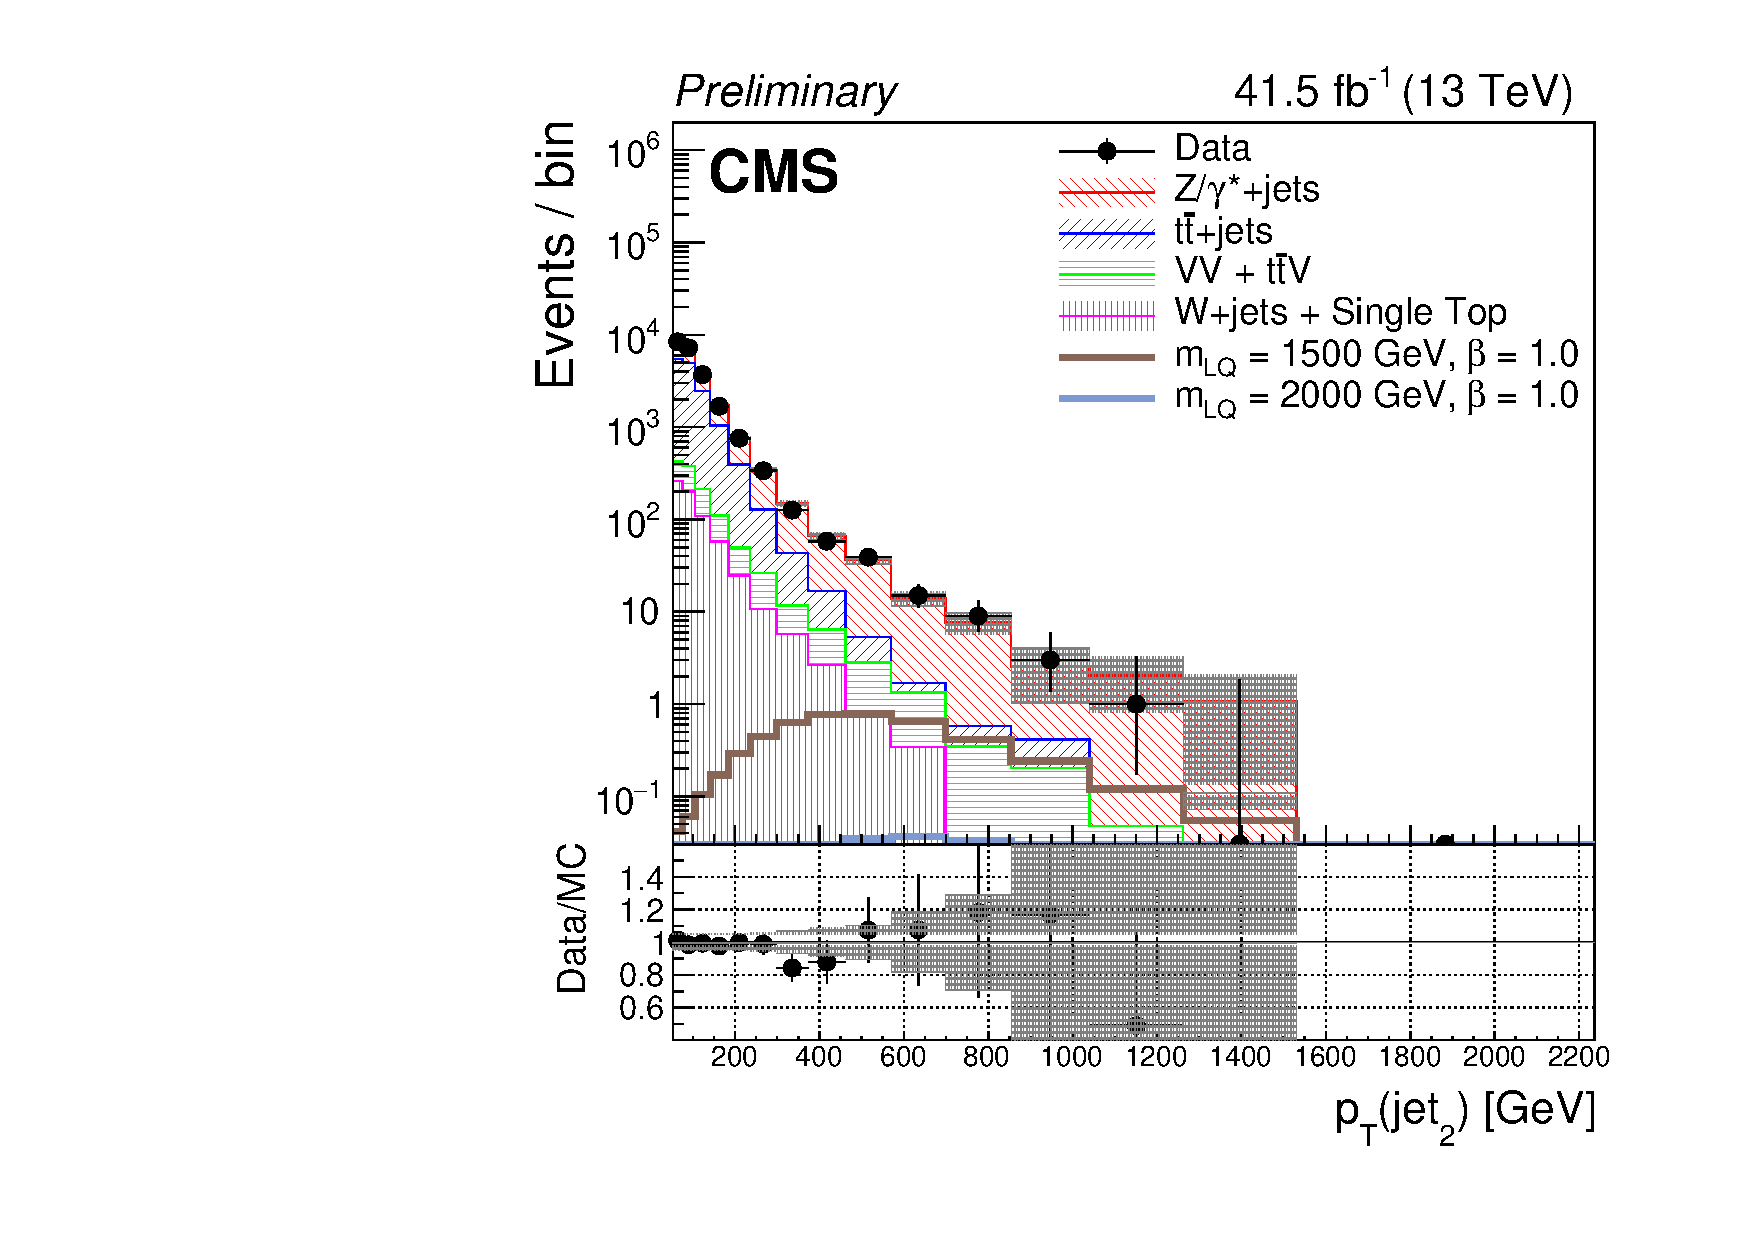
\includegraphics[width=.32\textwidth]{Images/Analysis/Results_2017_Unblinded/Plots/Preselection/BasicLQ_uujj_Pt_jet2_standard.pdf}}
       {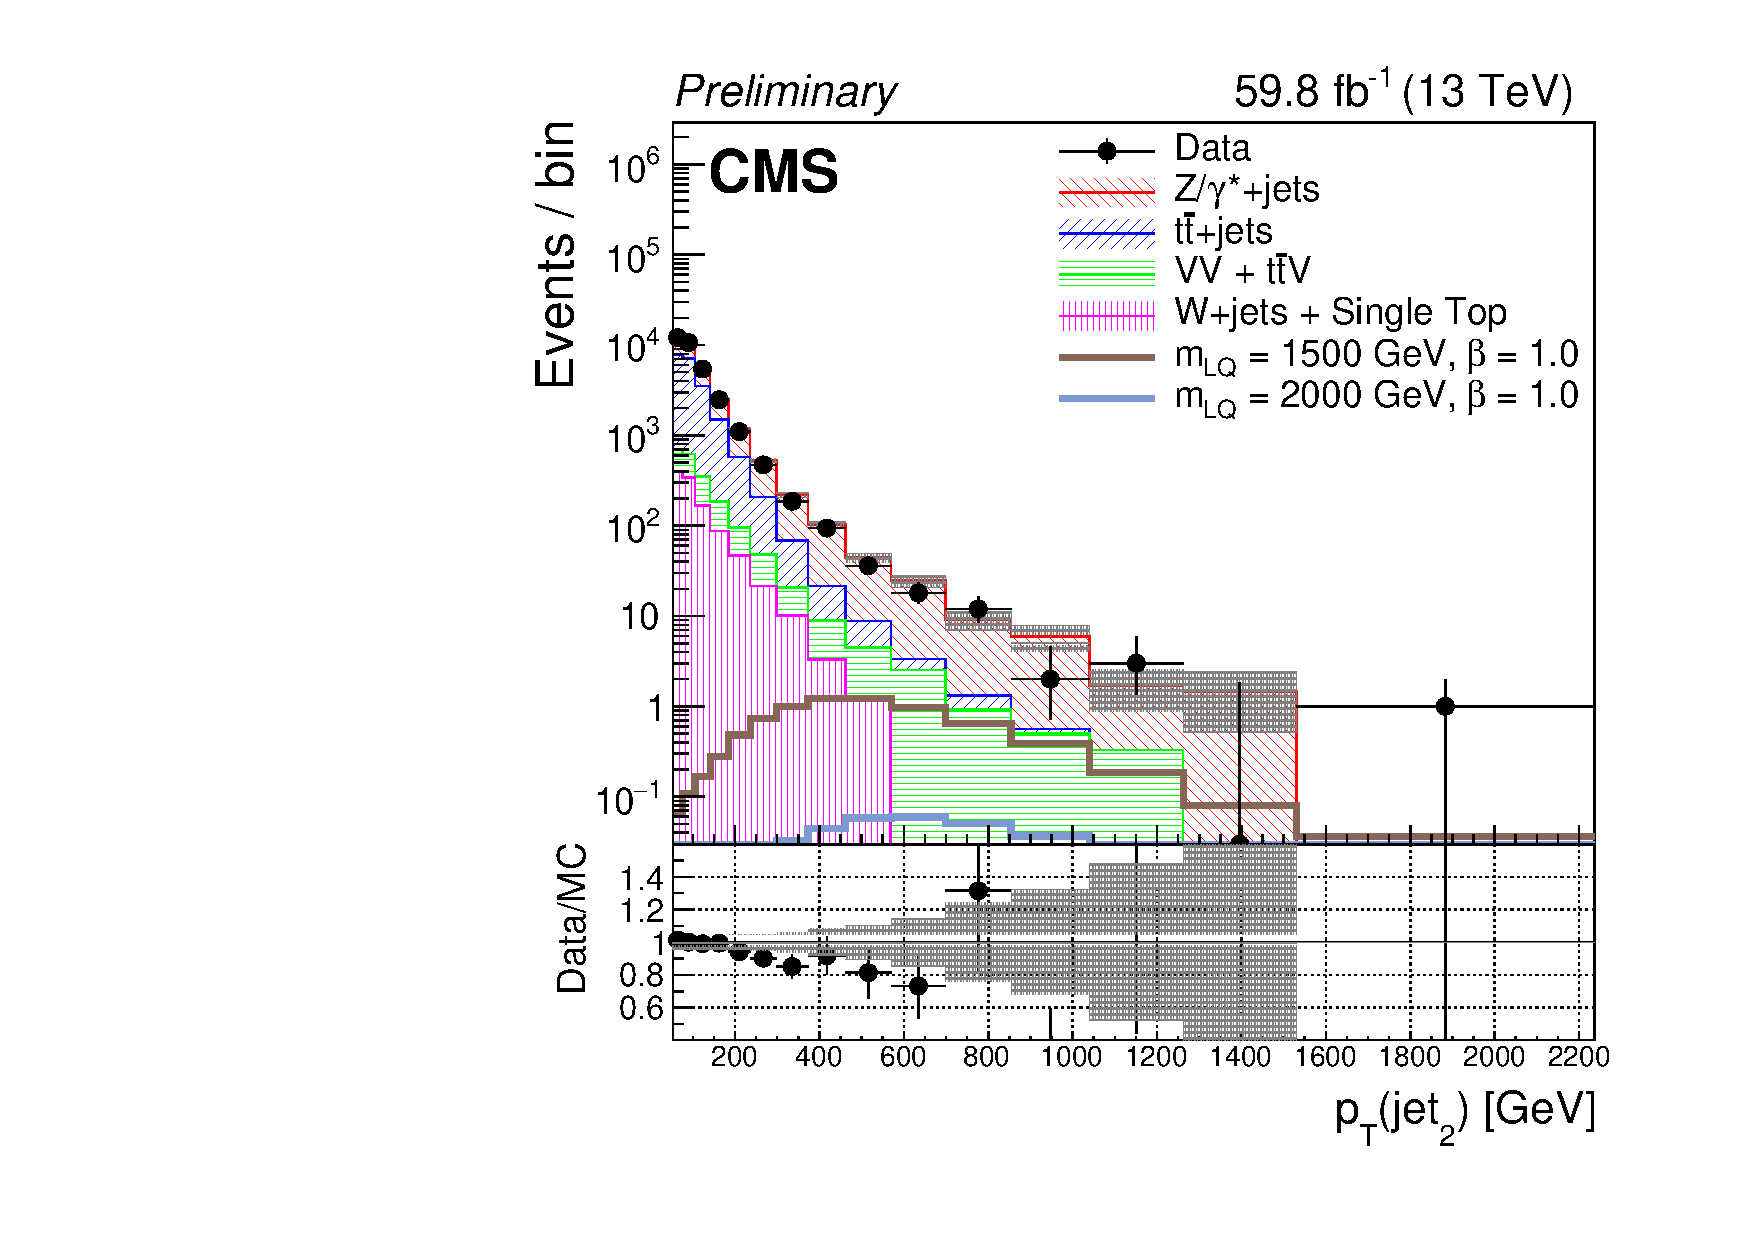
\includegraphics[width=.32\textwidth]{Images/Analysis/Results_2018_Unblinded/Plots/Preselection/BasicLQ_uujj_Pt_jet2_standard.pdf}}
       \caption{A comparison between distributions of observed data and SM expectation at preselection level. Left to right: 2016, 2017, 2018 data. Top to bottom: muon 1 \pt, muon 2 \pt, jet 1 \pt, and jet 2 \pt. Error bars on observed data points represent statistical uncertainties, and systematic uncertainties on SM expectation are shown by gray hashing.}
	\label{figapp:preselpt}
\end{figure}

\begin{figure}[H]
       \centering
       {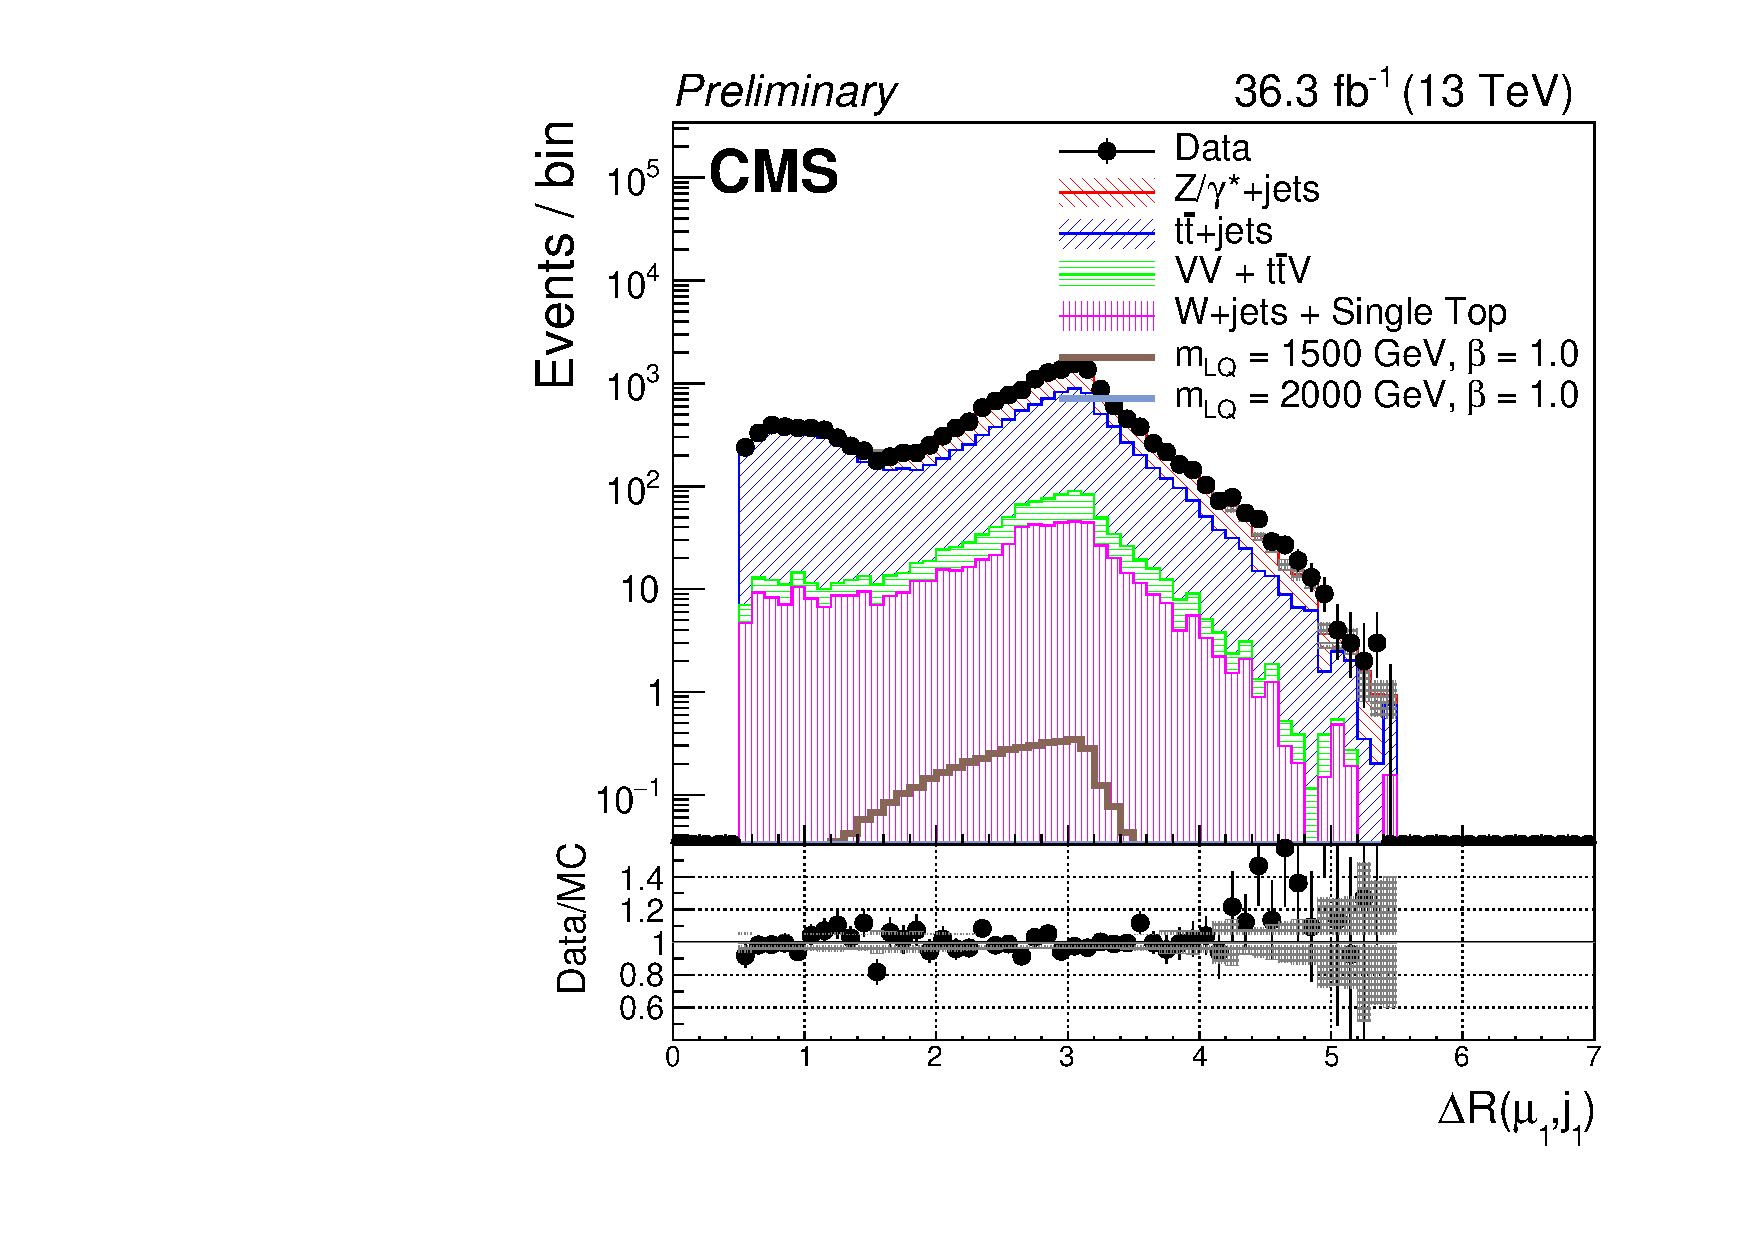
\includegraphics[width=0.32\textwidth]{Images/Analysis/Results_2016_Unblinded/Plots/Preselection/BasicLQ_uujj_DR_muon1jet1_standard.pdf}}
       {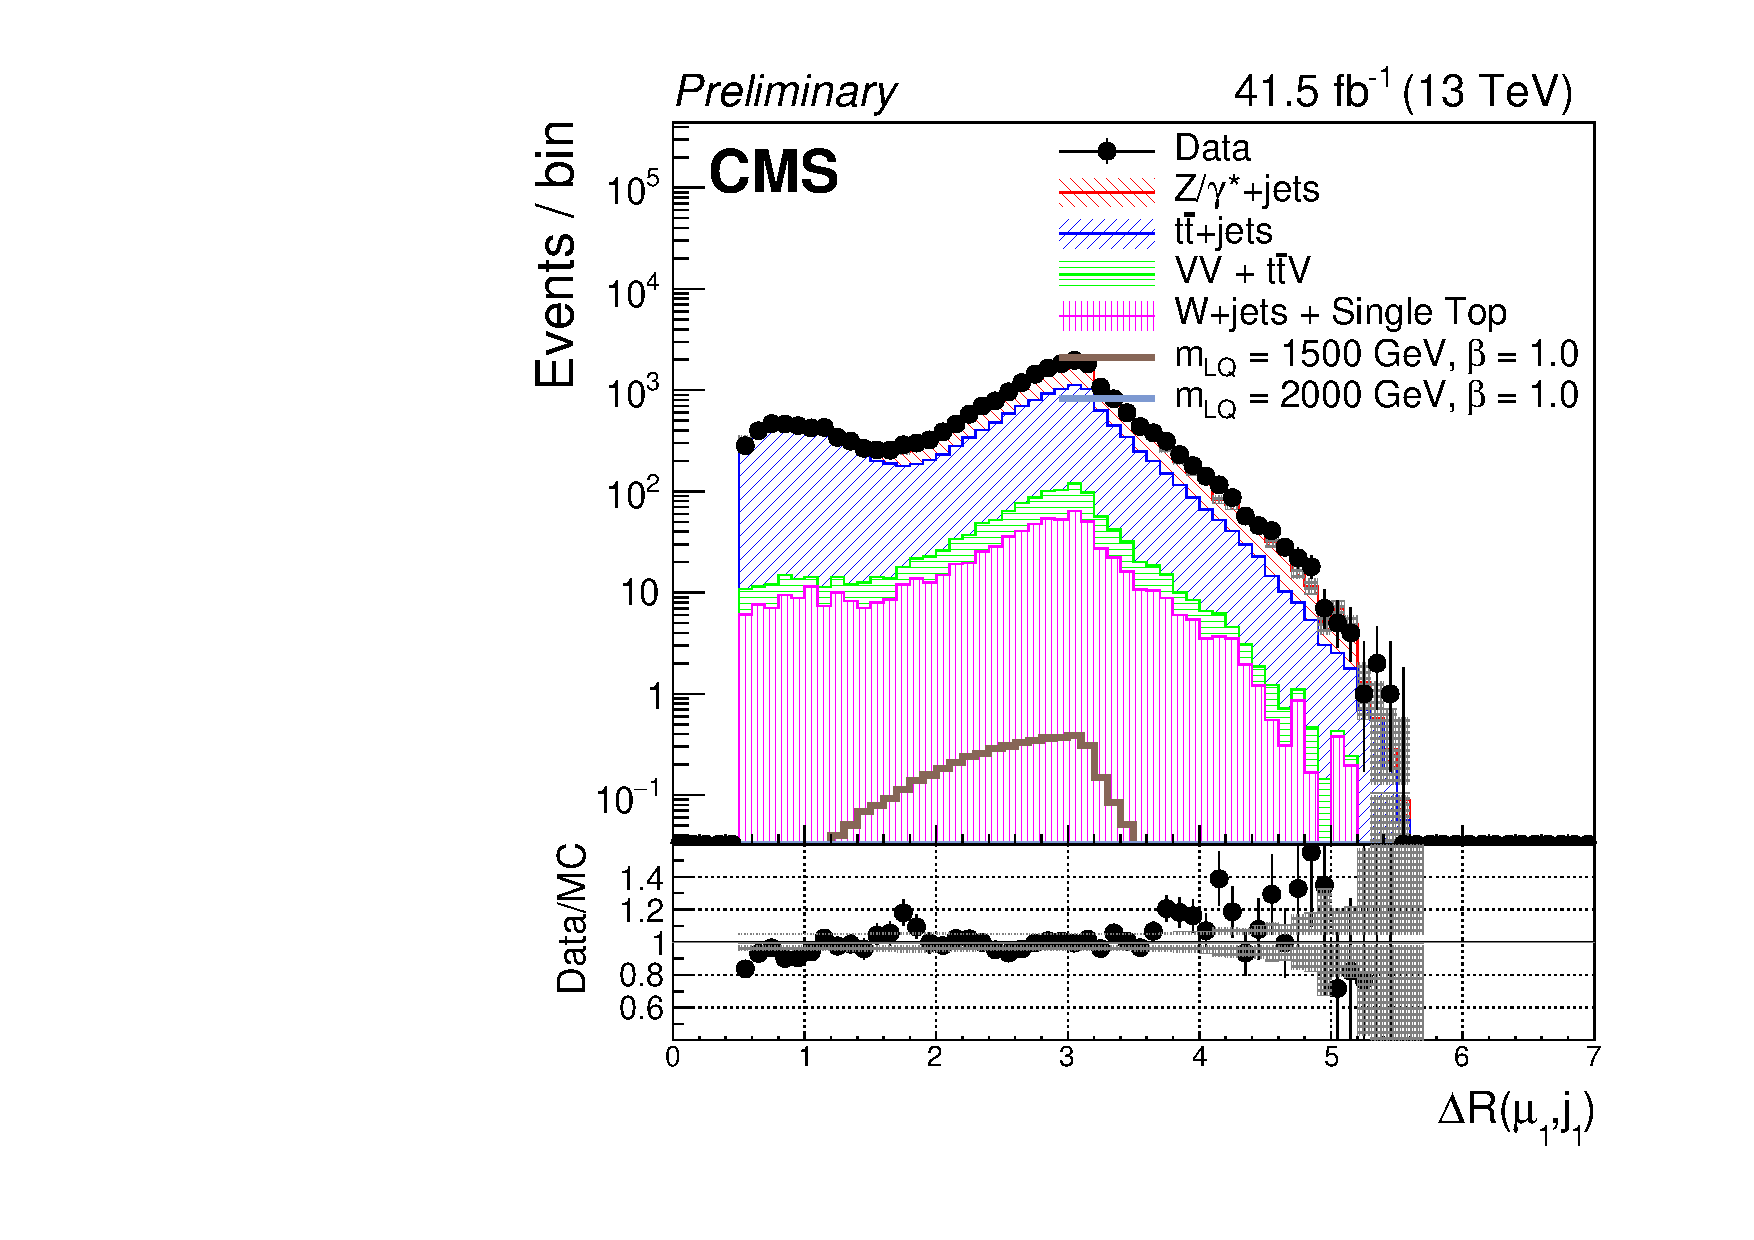
\includegraphics[width=0.32\textwidth]{Images/Analysis/Results_2017_Unblinded/Plots/Preselection/BasicLQ_uujj_DR_muon1jet1_standard.pdf}}
       {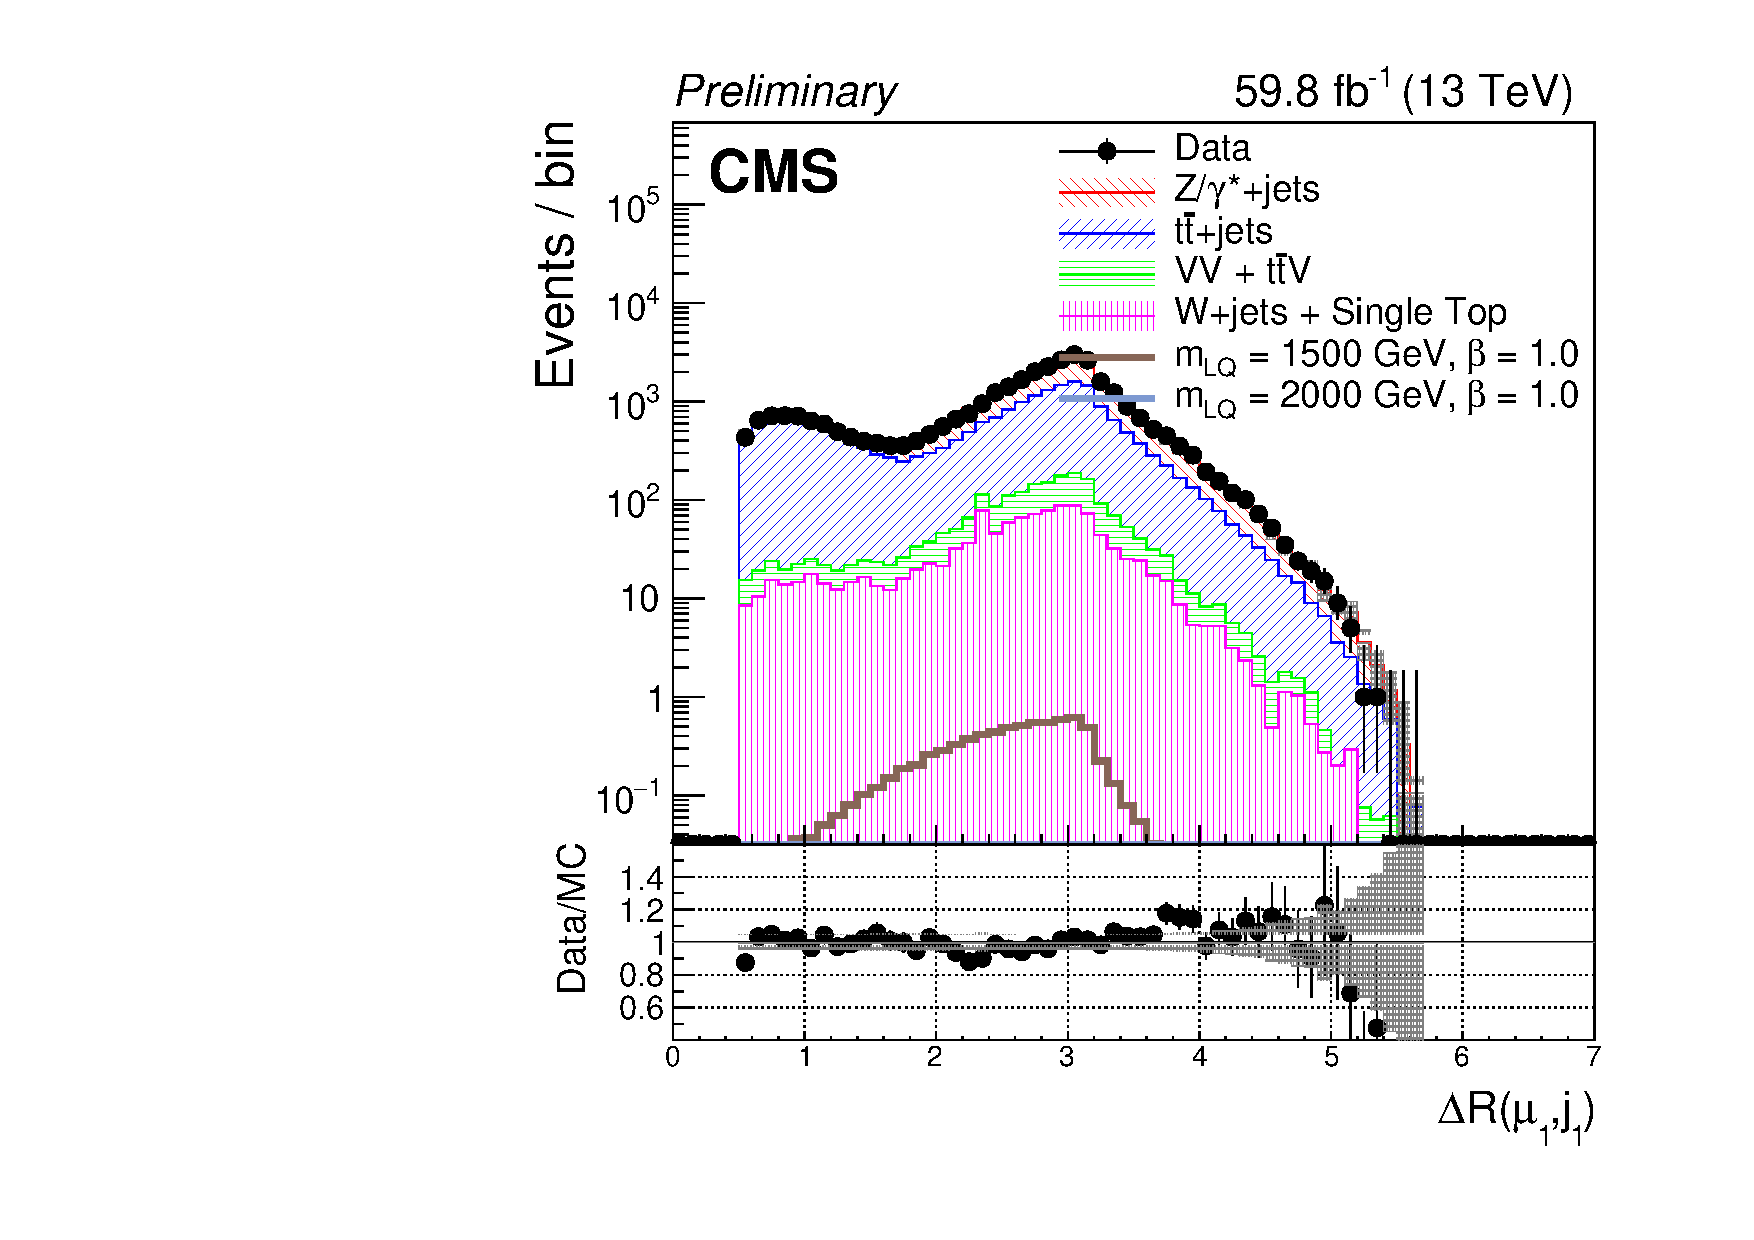
\includegraphics[width=0.32\textwidth]{Images/Analysis/Results_2018_Unblinded/Plots/Preselection/BasicLQ_uujj_DR_muon1jet1_standard.pdf}}
       {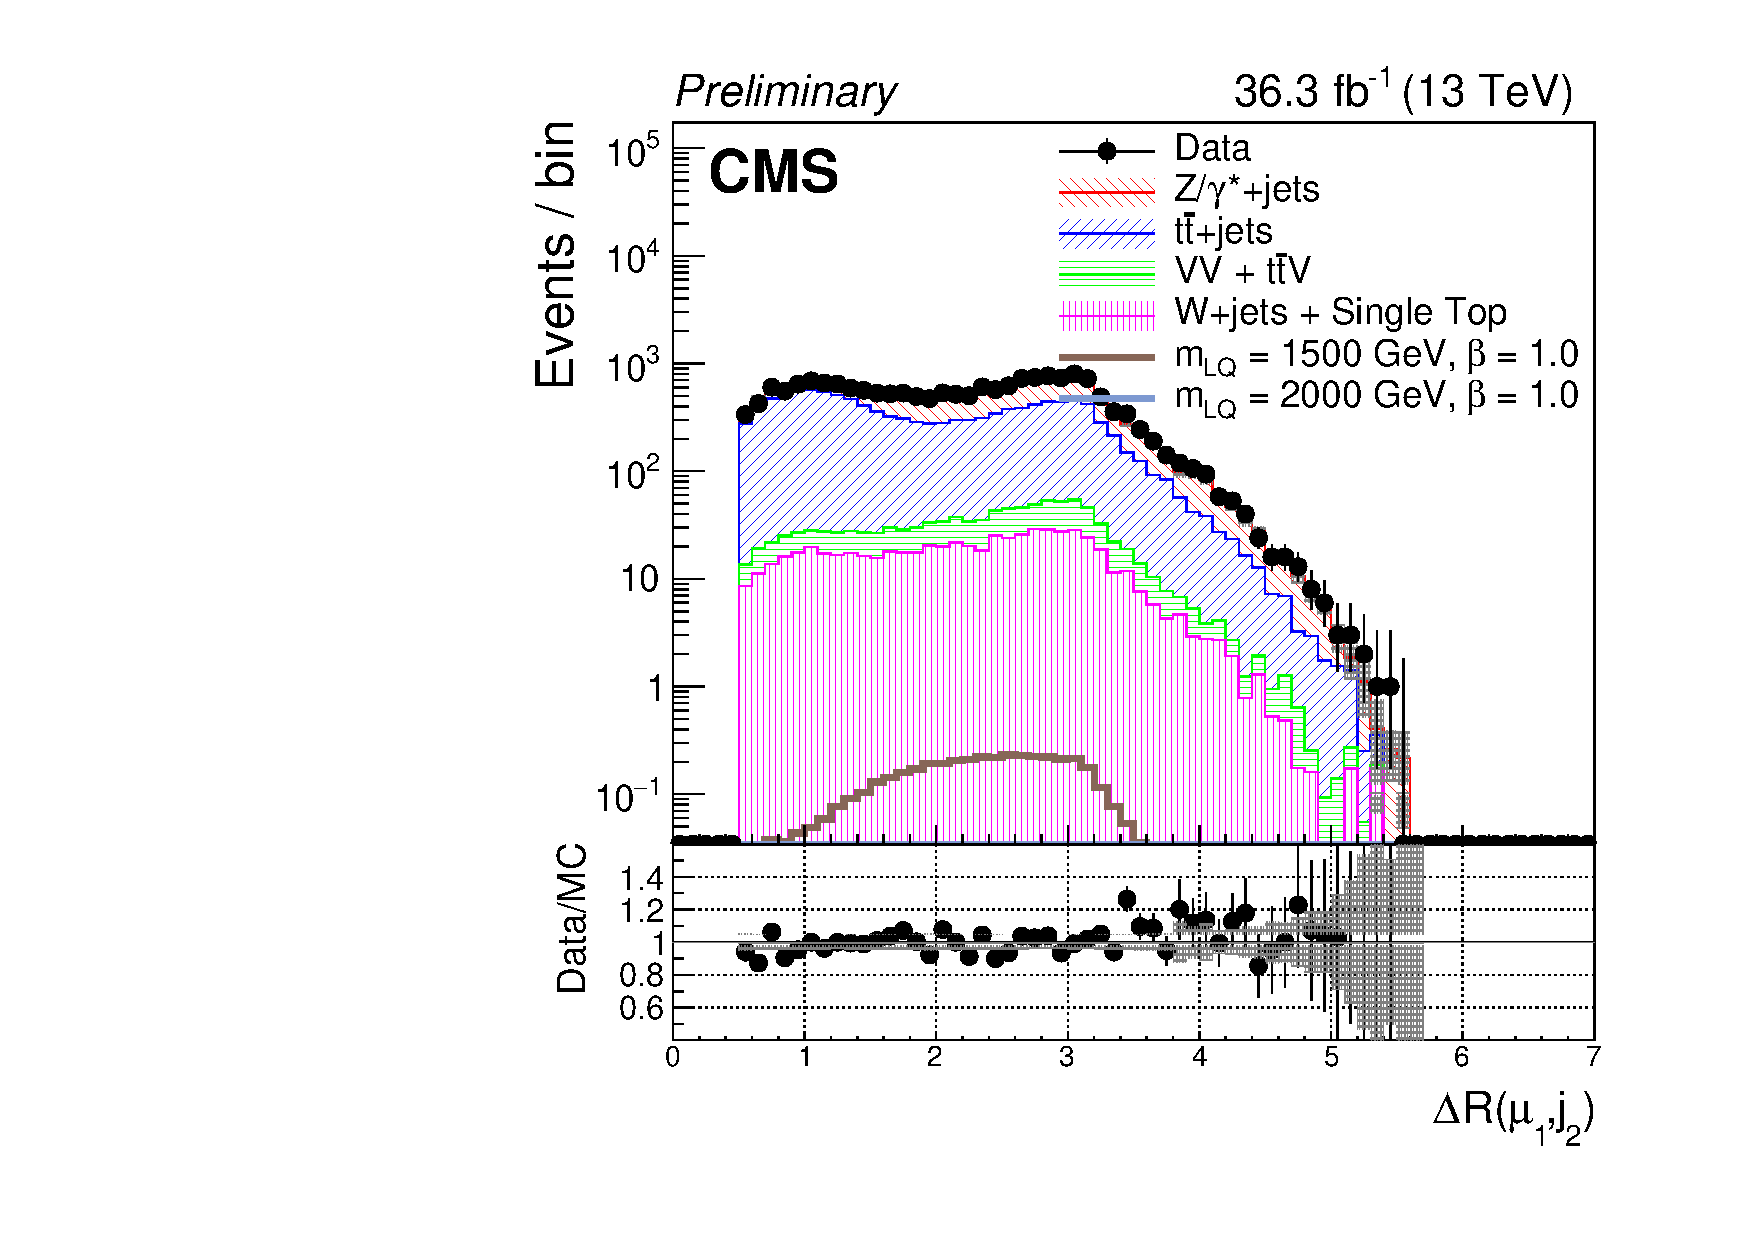
\includegraphics[width=0.32\textwidth]{Images/Analysis/Results_2016_Unblinded/Plots/Preselection/BasicLQ_uujj_DR_muon1jet2_standard.pdf}}
       {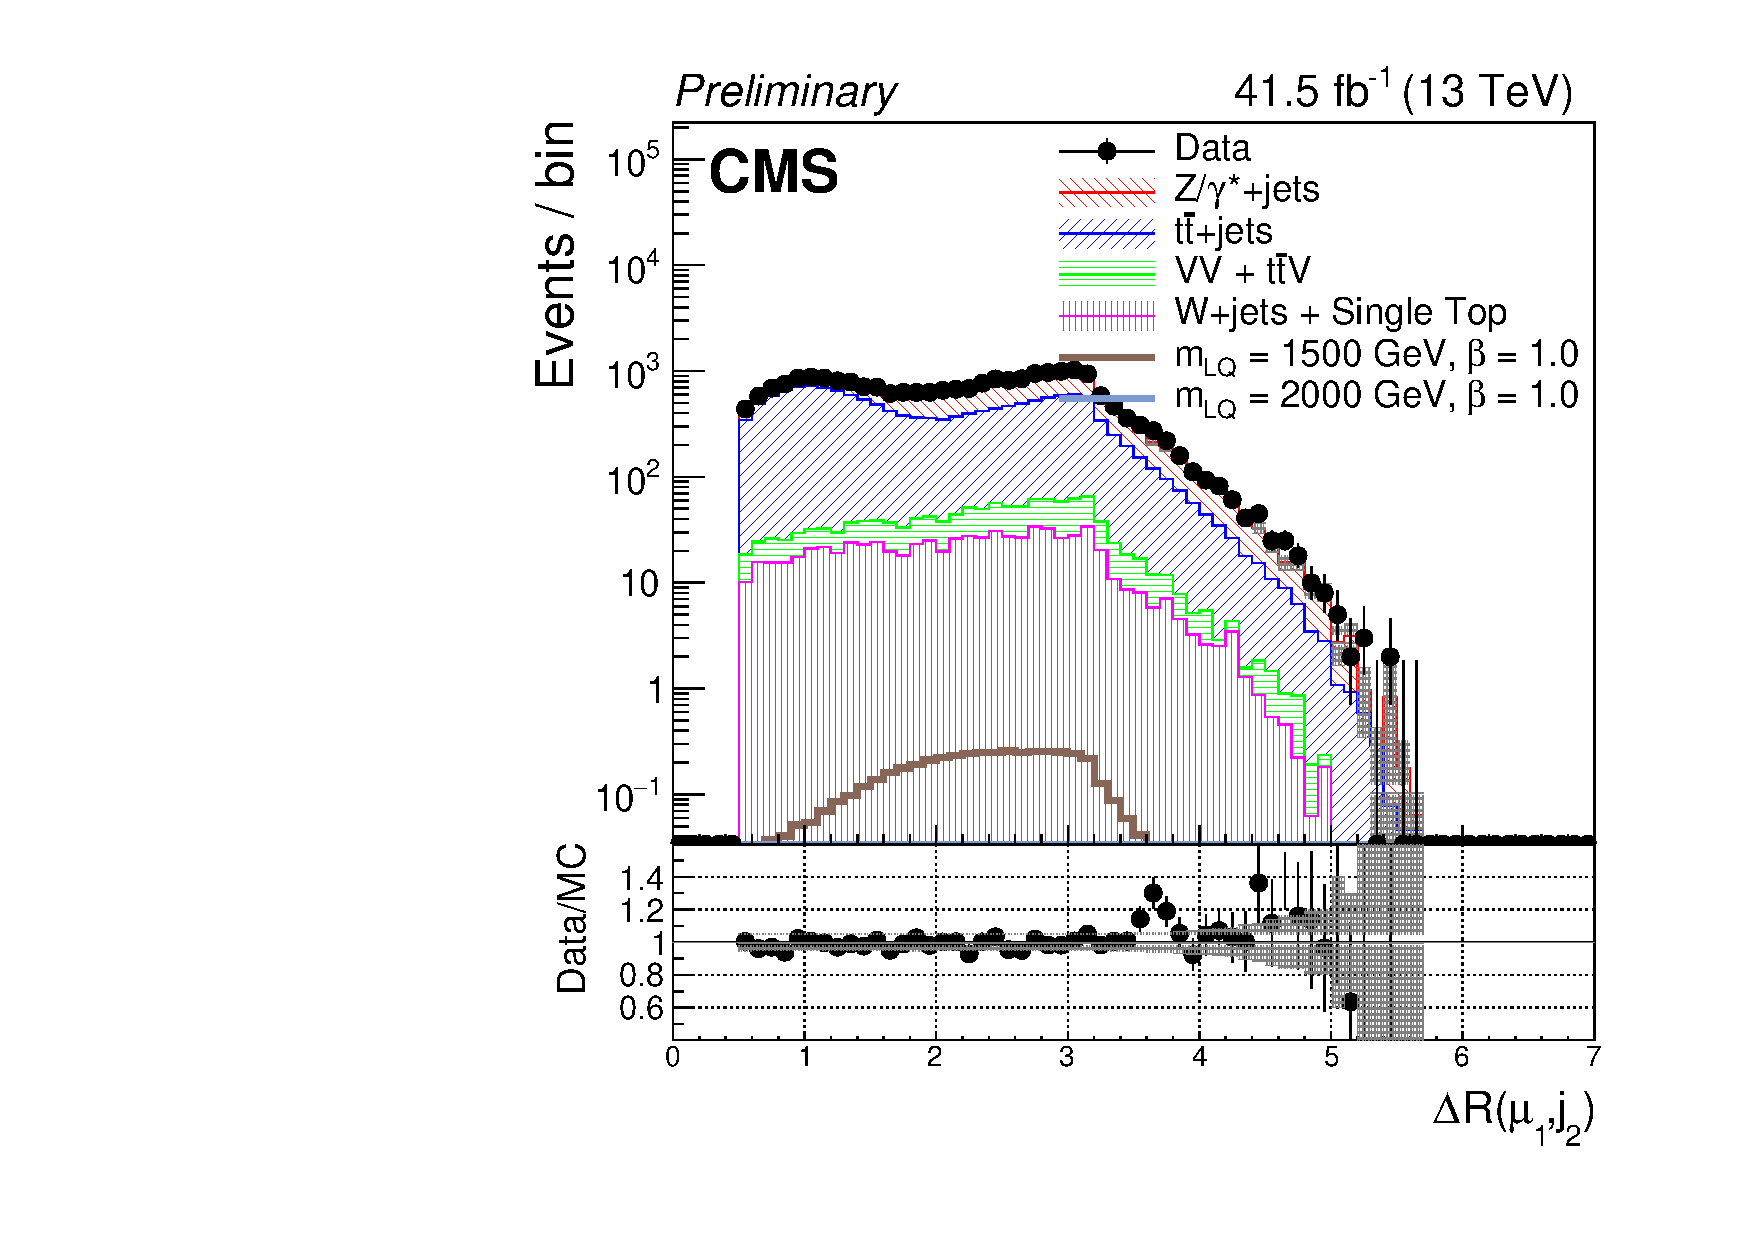
\includegraphics[width=0.32\textwidth]{Images/Analysis/Results_2017_Unblinded/Plots/Preselection/BasicLQ_uujj_DR_muon1jet2_standard.pdf}}
       {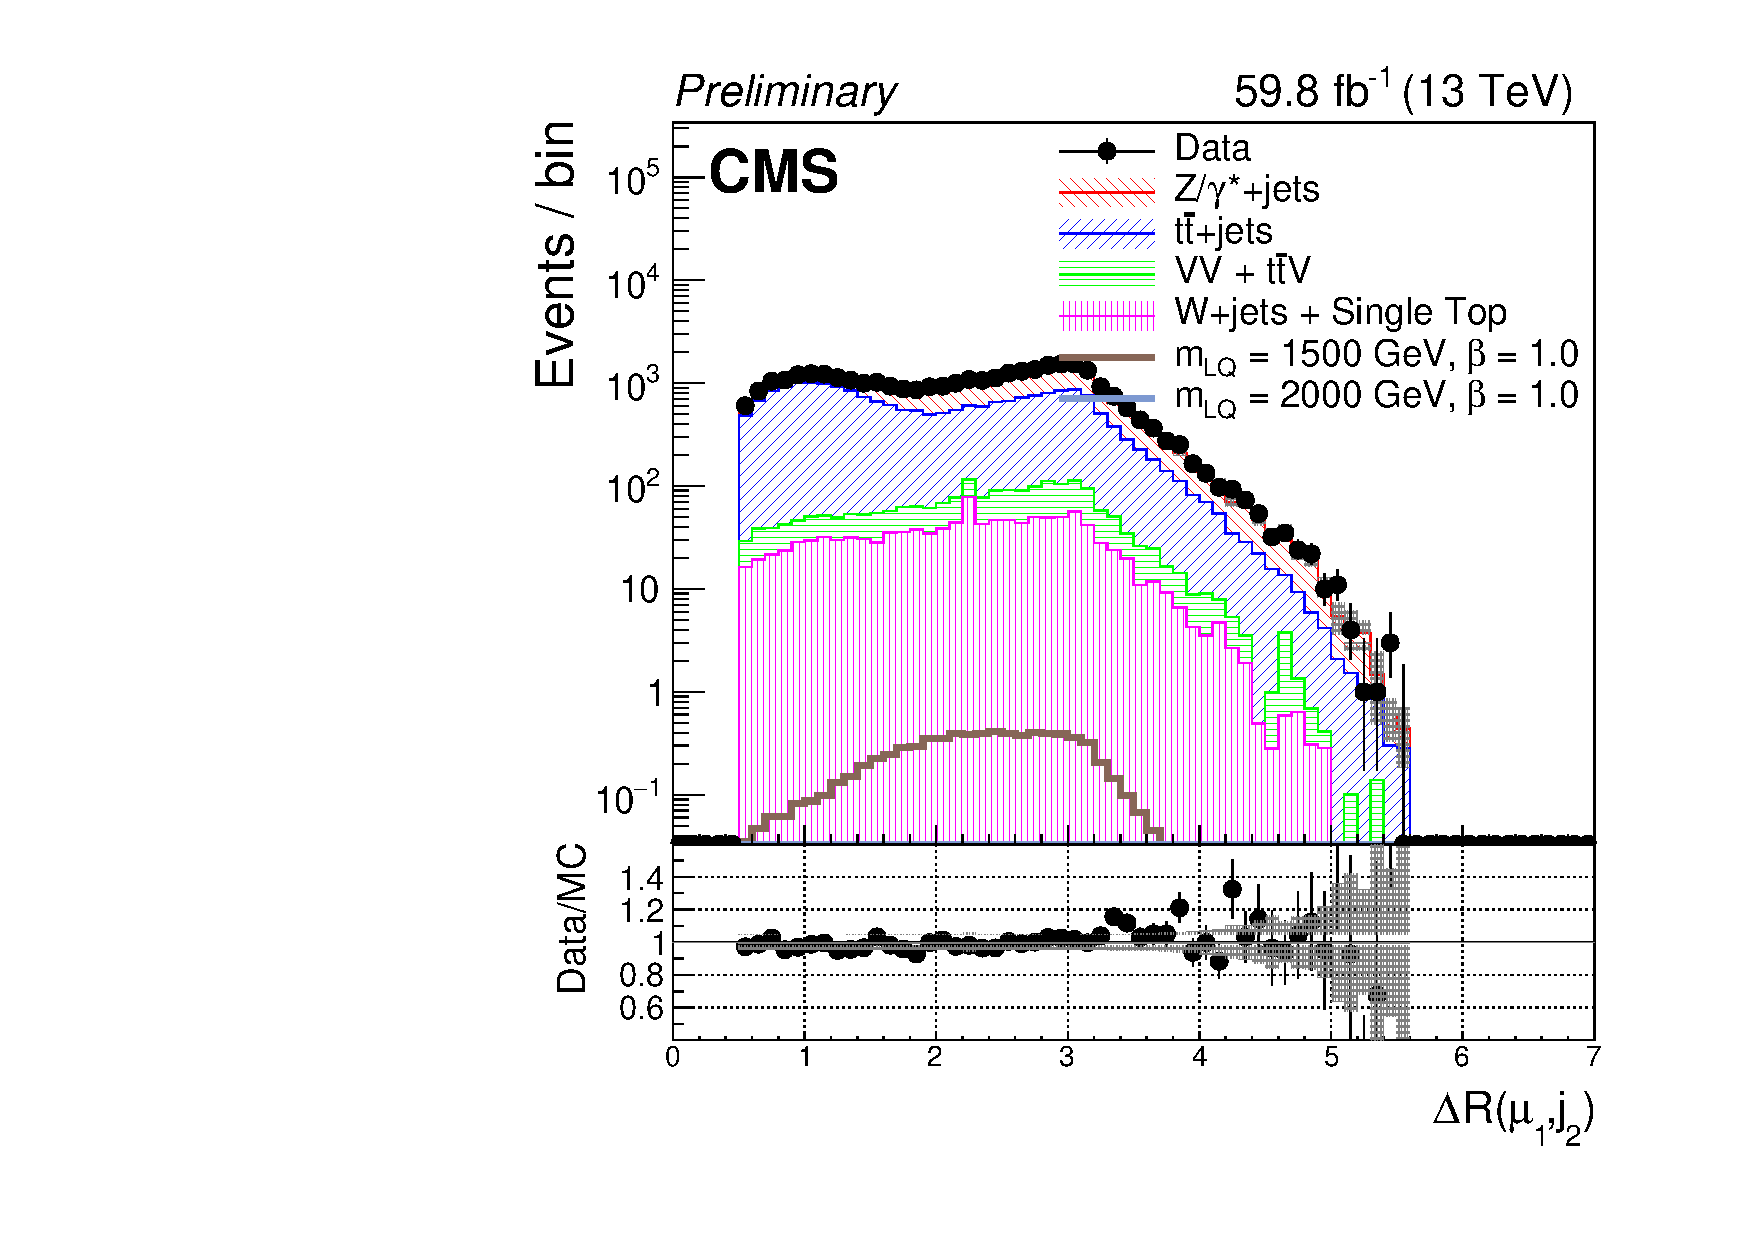
\includegraphics[width=0.32\textwidth]{Images/Analysis/Results_2018_Unblinded/Plots/Preselection/BasicLQ_uujj_DR_muon1jet2_standard.pdf}}
       {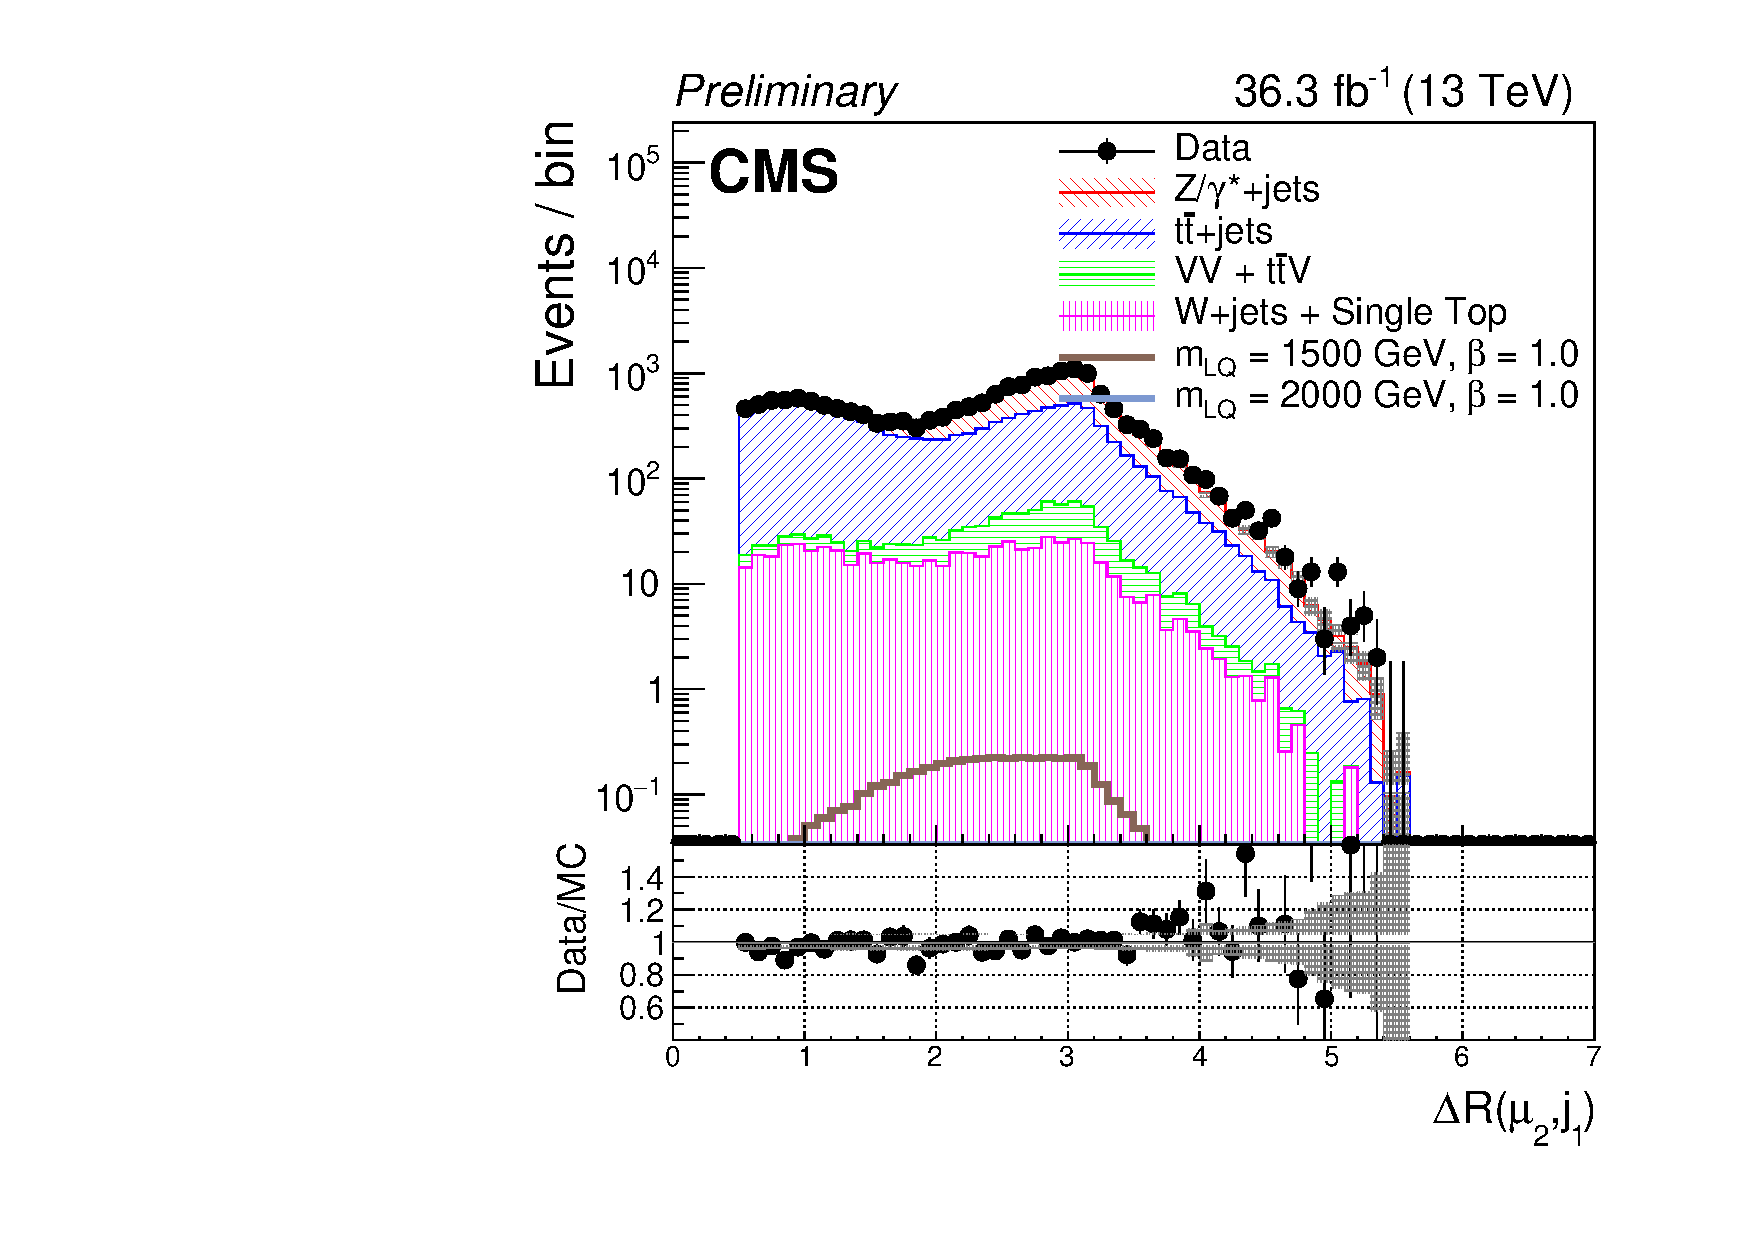
\includegraphics[width=0.32\textwidth]{Images/Analysis/Results_2016_Unblinded/Plots/Preselection/BasicLQ_uujj_DR_muon2jet1_standard.pdf}}
       {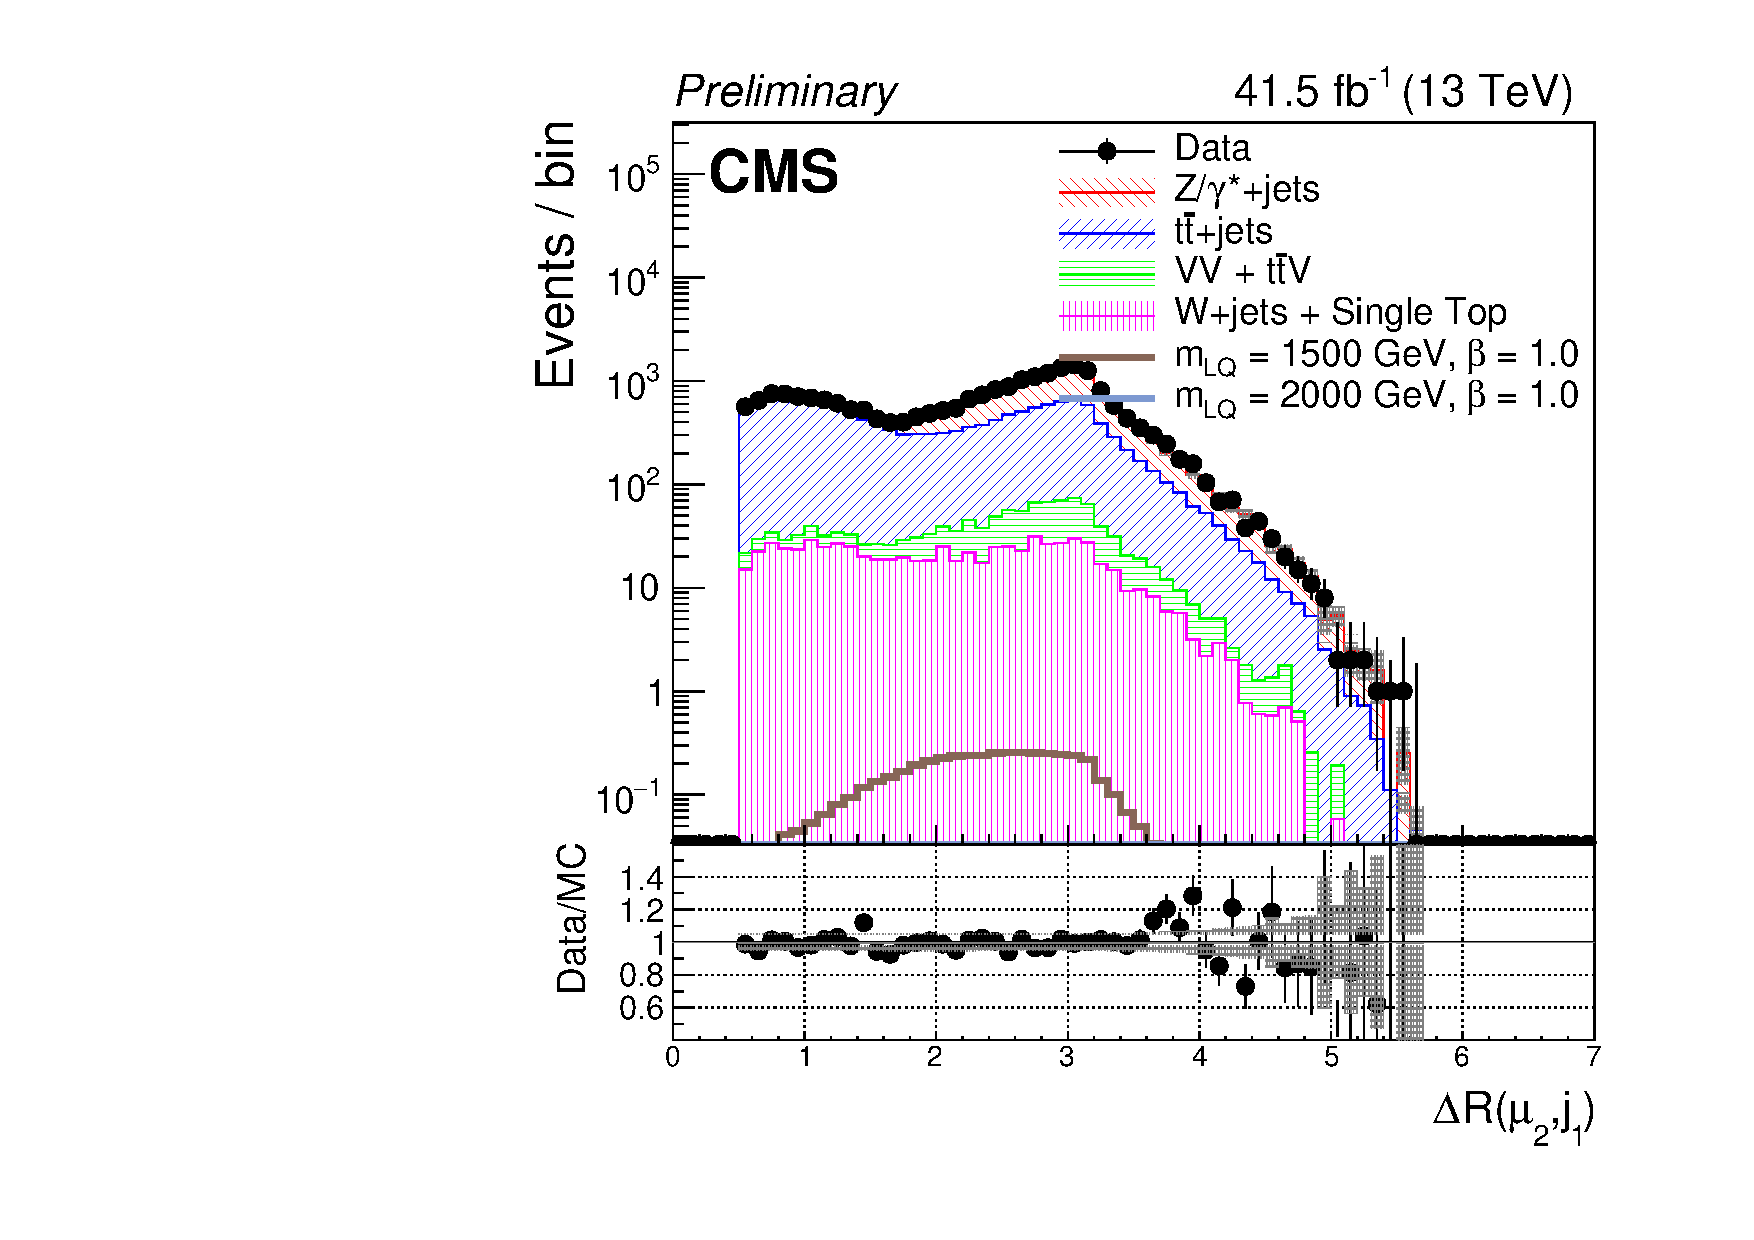
\includegraphics[width=0.32\textwidth]{Images/Analysis/Results_2017_Unblinded/Plots/Preselection/BasicLQ_uujj_DR_muon2jet1_standard.pdf}}
       {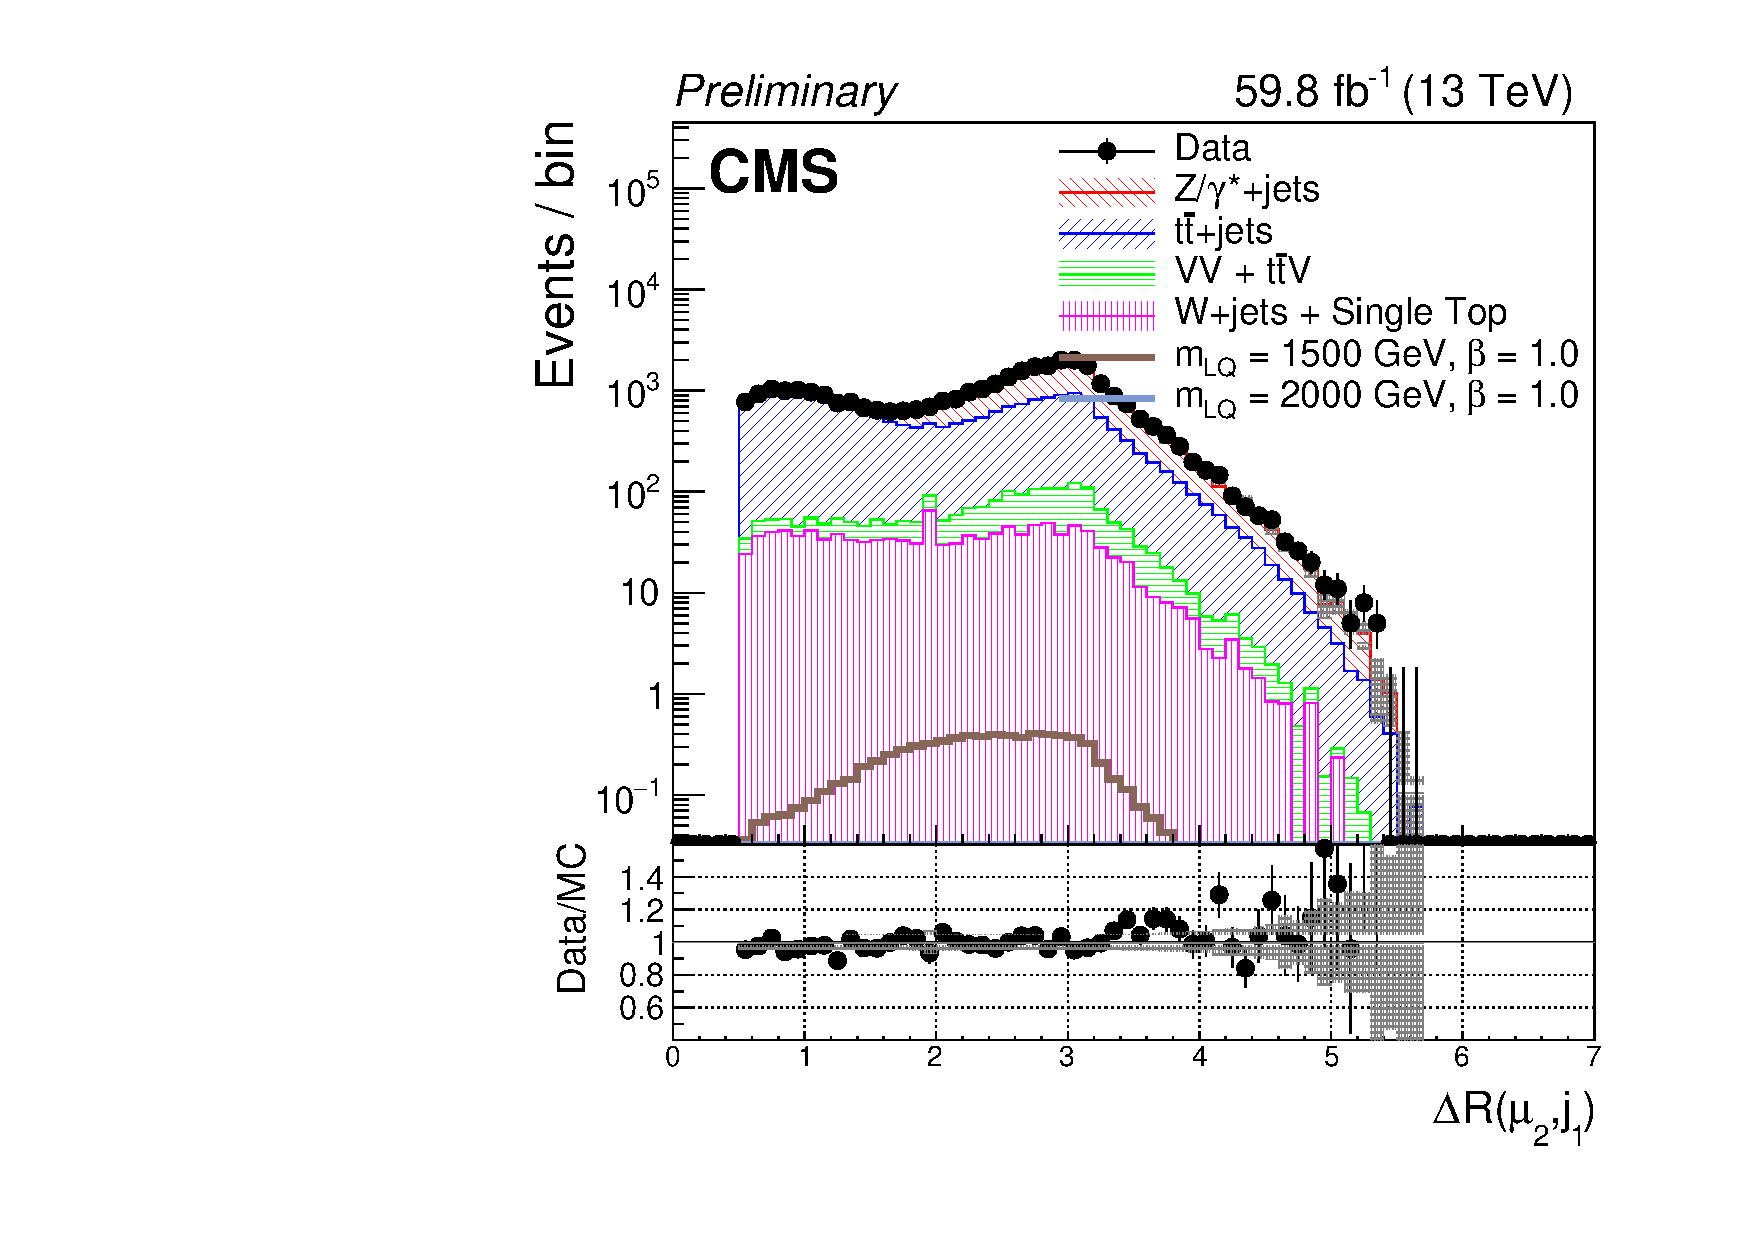
\includegraphics[width=0.32\textwidth]{Images/Analysis/Results_2018_Unblinded/Plots/Preselection/BasicLQ_uujj_DR_muon2jet1_standard.pdf}}
       {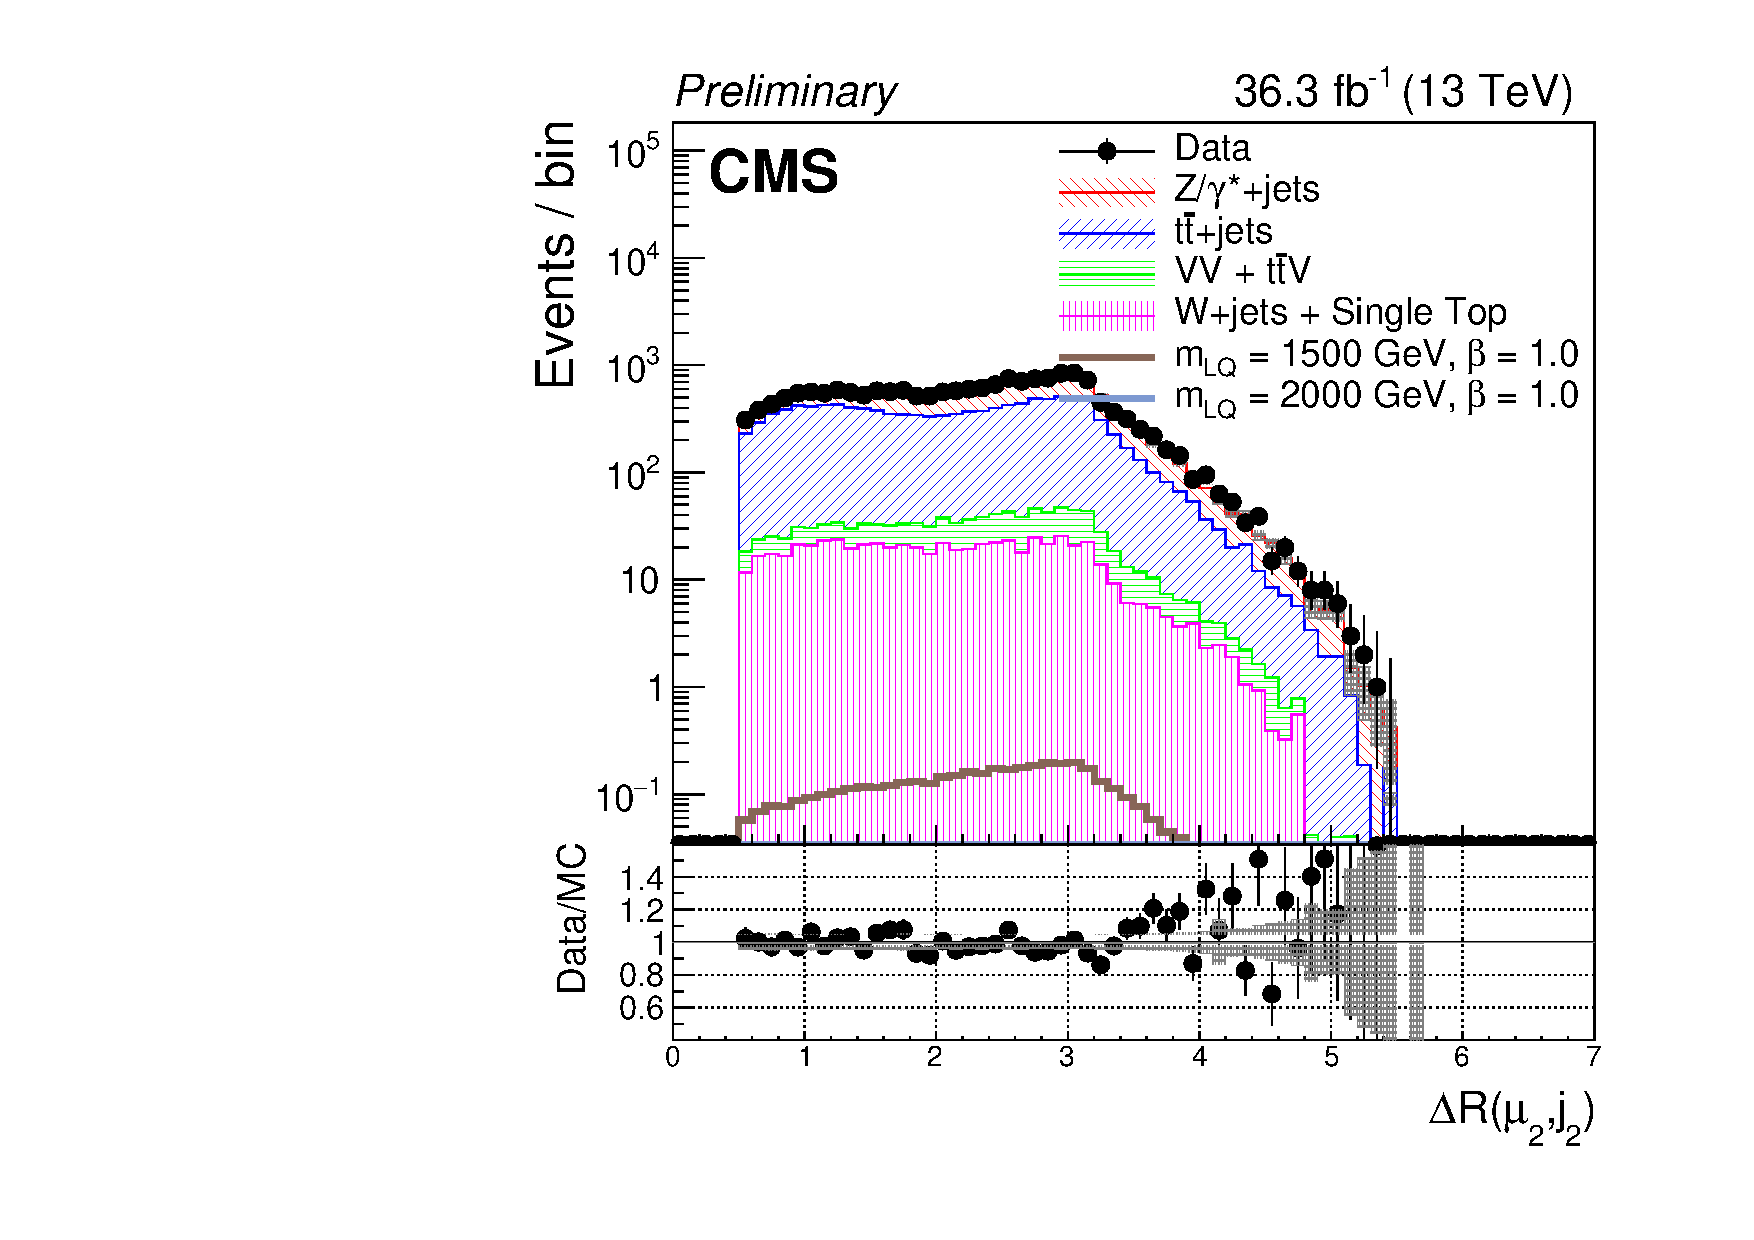
\includegraphics[width=0.32\textwidth]{Images/Analysis/Results_2016_Unblinded/Plots/Preselection/BasicLQ_uujj_DR_muon2jet2_standard.pdf}}
       {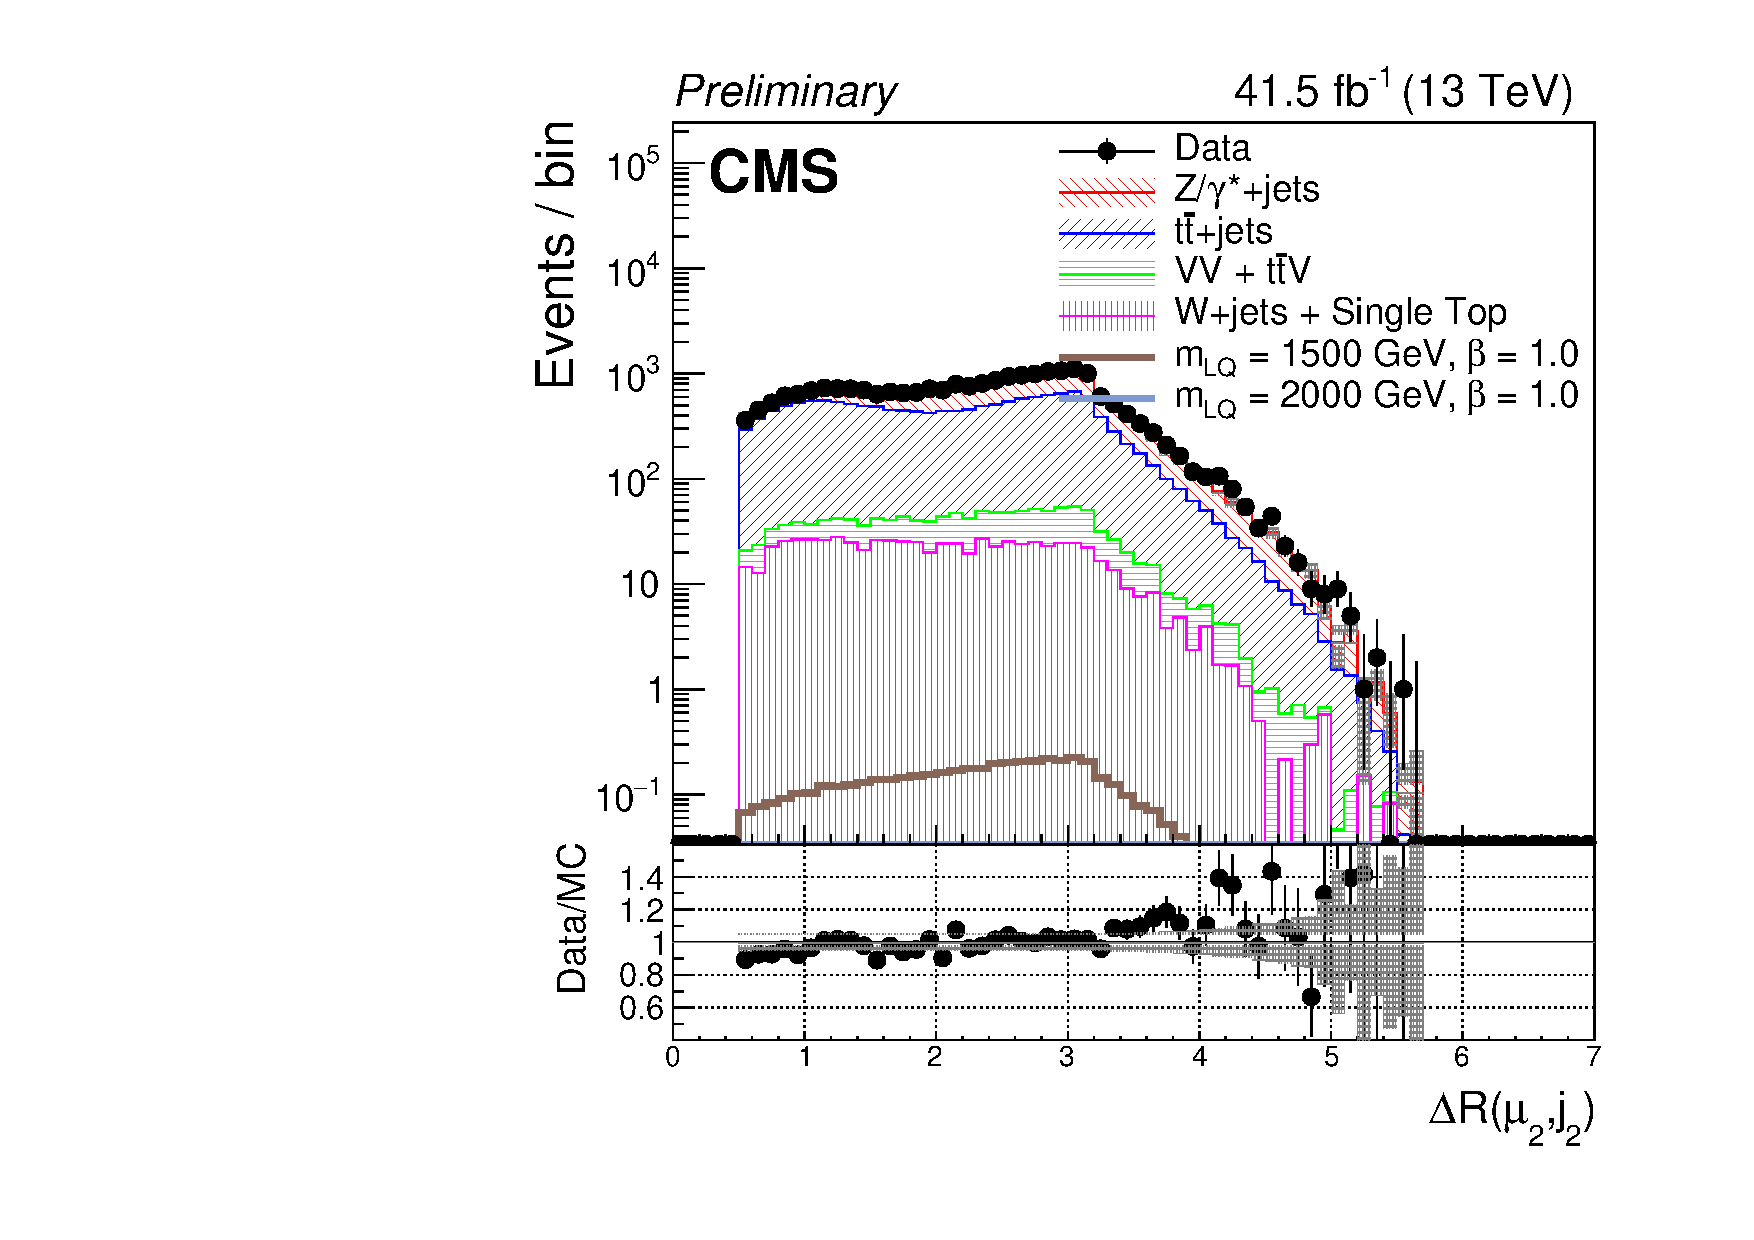
\includegraphics[width=0.32\textwidth]{Images/Analysis/Results_2017_Unblinded/Plots/Preselection/BasicLQ_uujj_DR_muon2jet2_standard.pdf}}
       {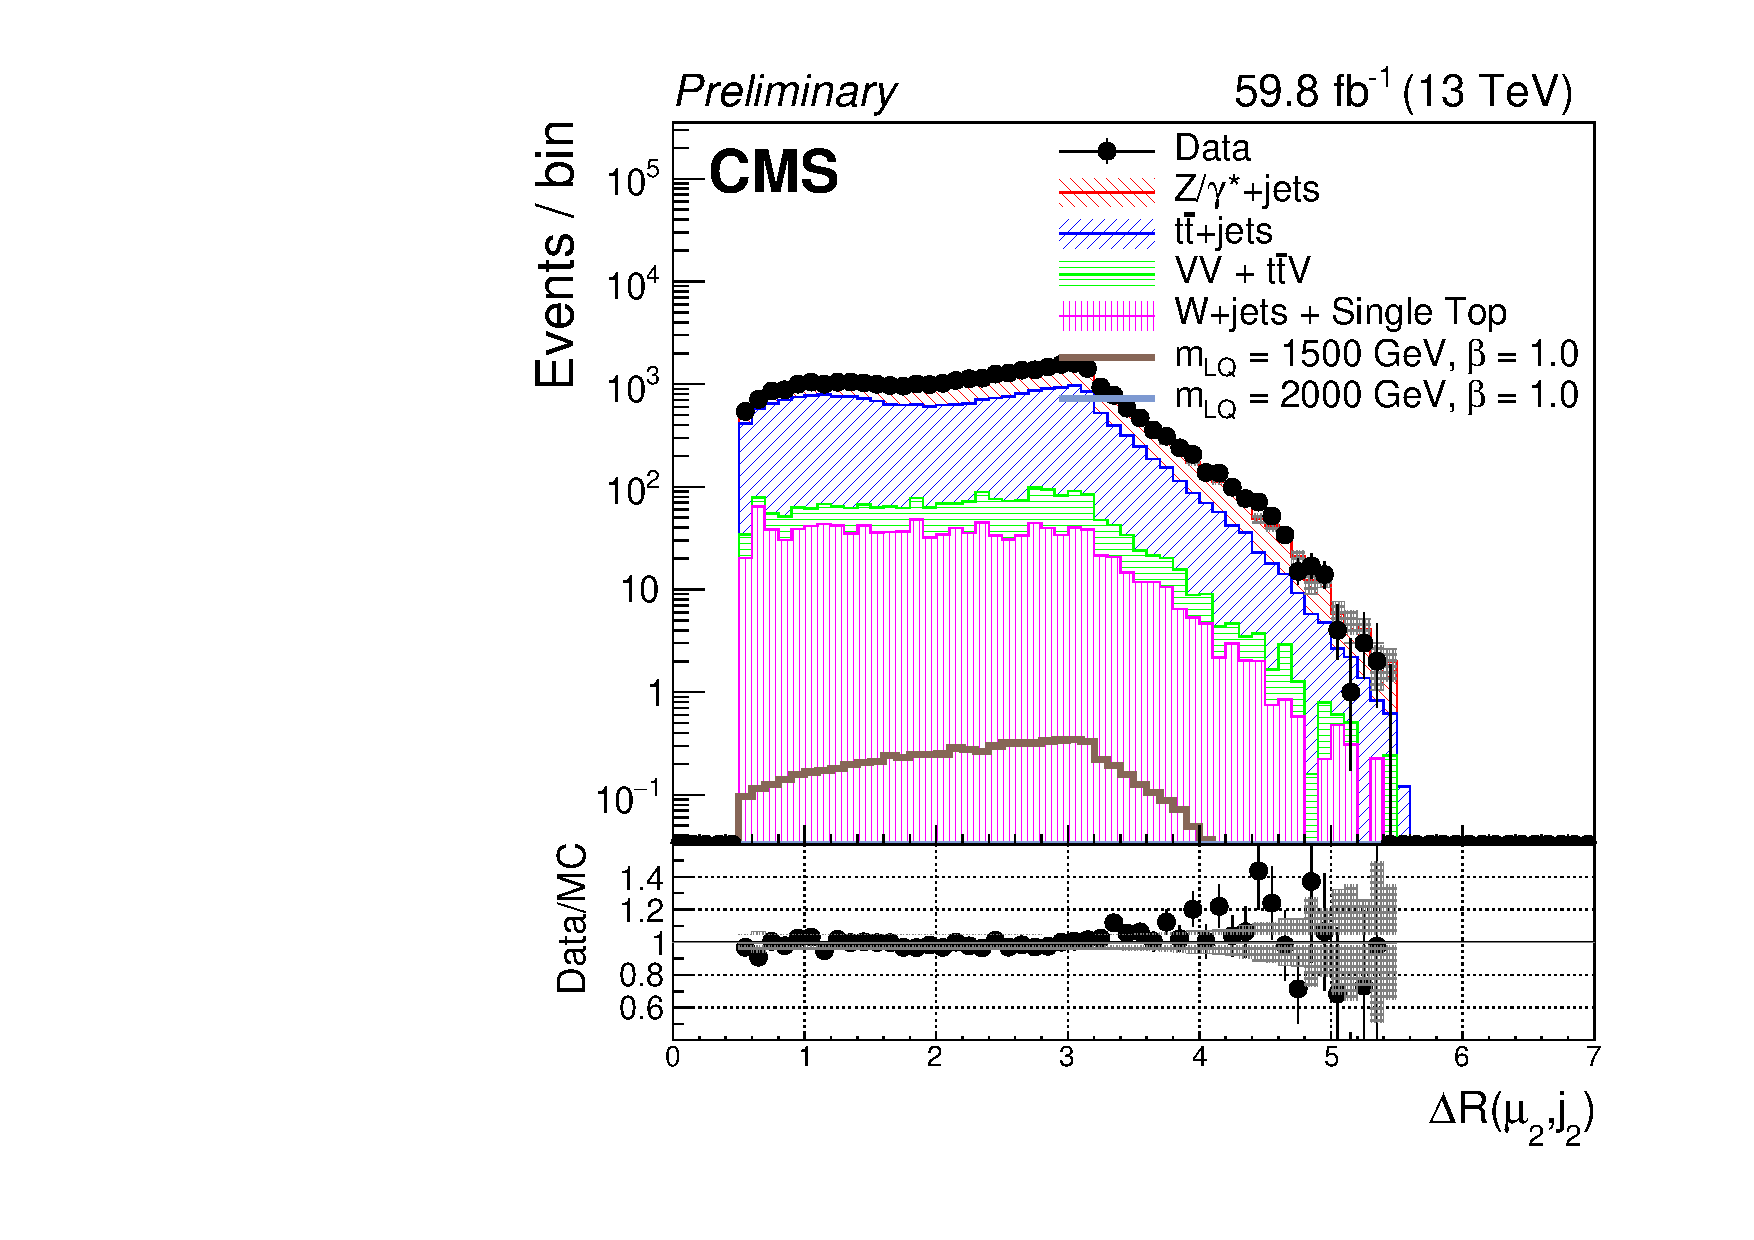
\includegraphics[width=0.32\textwidth]{Images/Analysis/Results_2018_Unblinded/Plots/Preselection/BasicLQ_uujj_DR_muon2jet2_standard.pdf}}
       \caption{A comparison between distributions of observed data and SM expectation at preselection level. Left to right: 2016, 2017, 2018 data. Top to bottom: \DR between muon 1 and jet 1, \DR between muon 1 and jet 2, \DR between muon 2 and jet 1, and \DR between muon 2 and jet 2. Error bars on observed data points represent statistical uncertainties, and systematic uncertainties on SM expectation are shown by gray hashing.}
       \label{figapp:preseldr}
\end{figure}

\begin{figure}[H]
       \centering
       {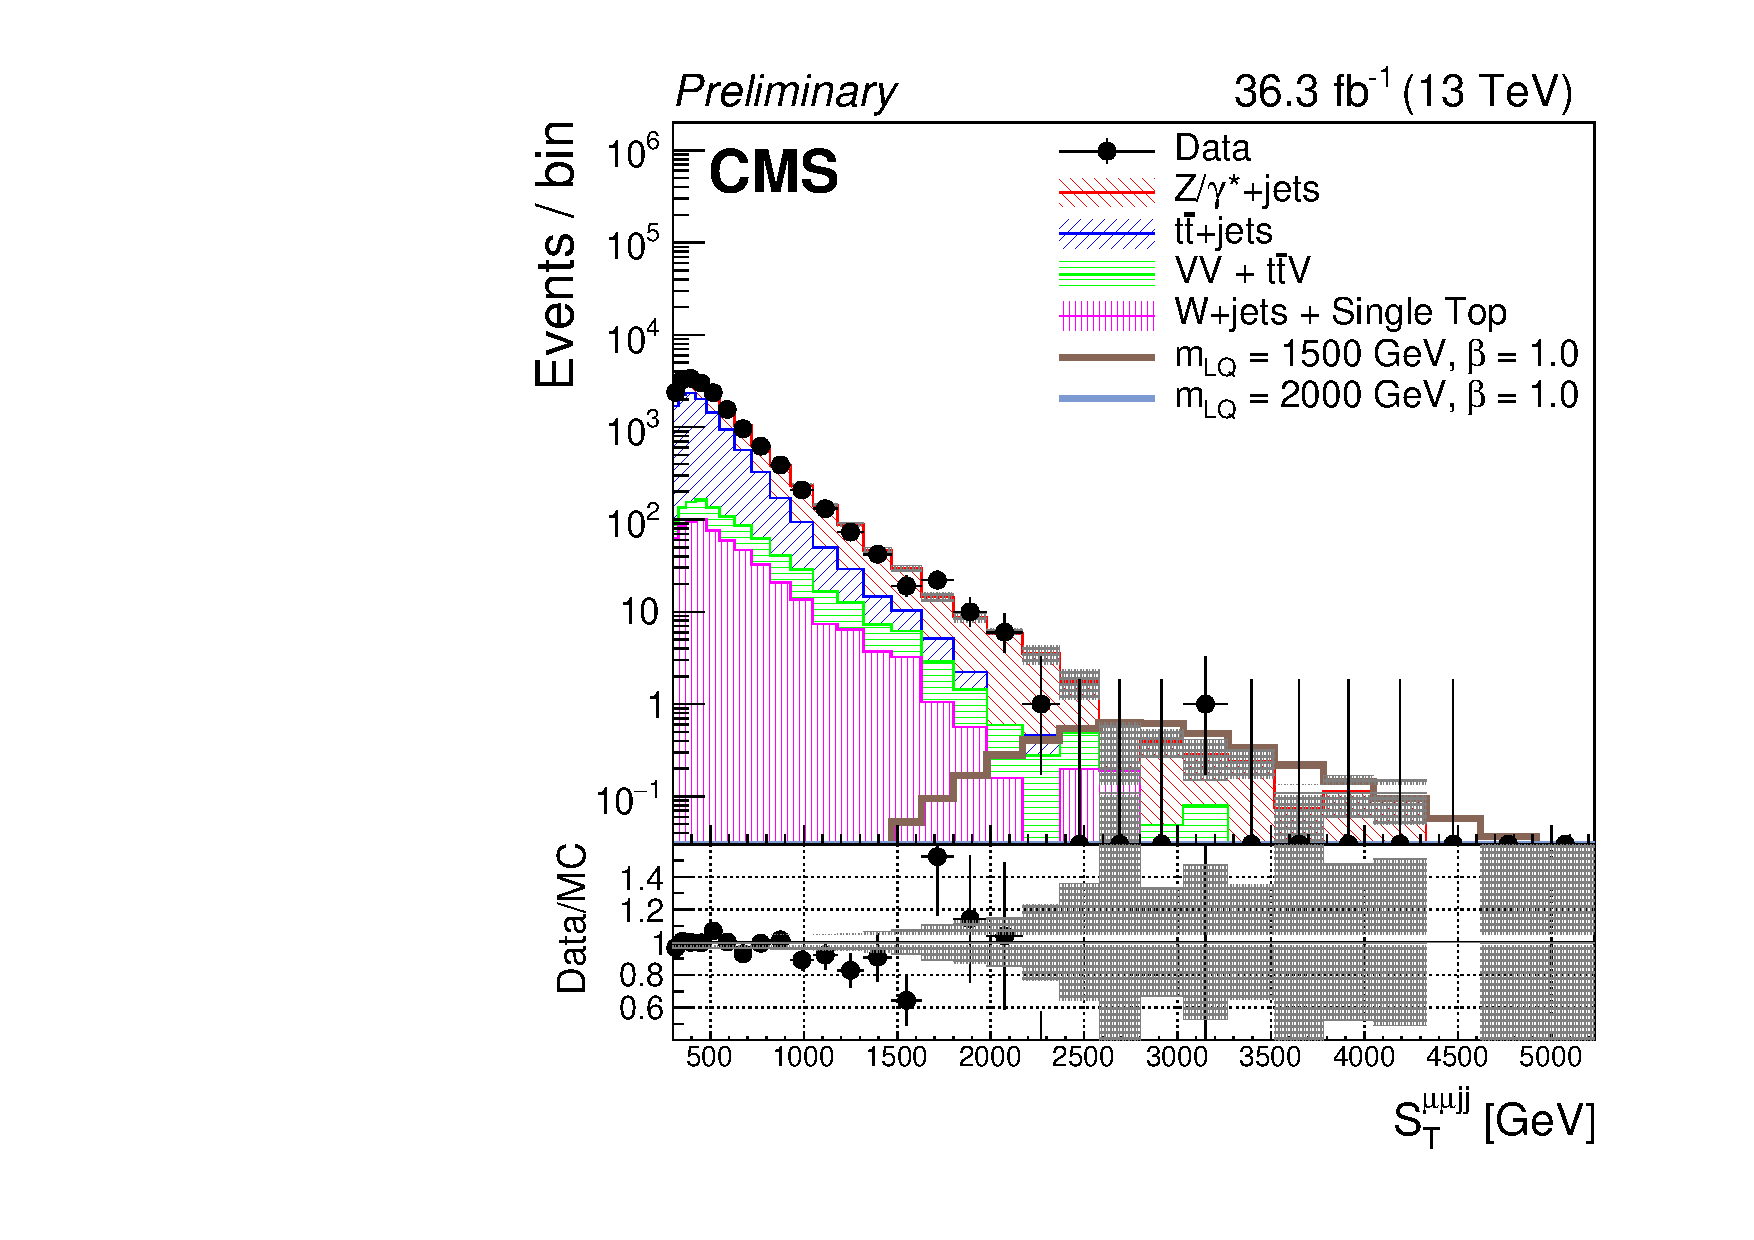
\includegraphics[width=.32\textwidth]{Images/Analysis/Results_2016_Unblinded/Plots/Preselection/BasicLQ_uujj_St_uujj_standard.pdf}}
       {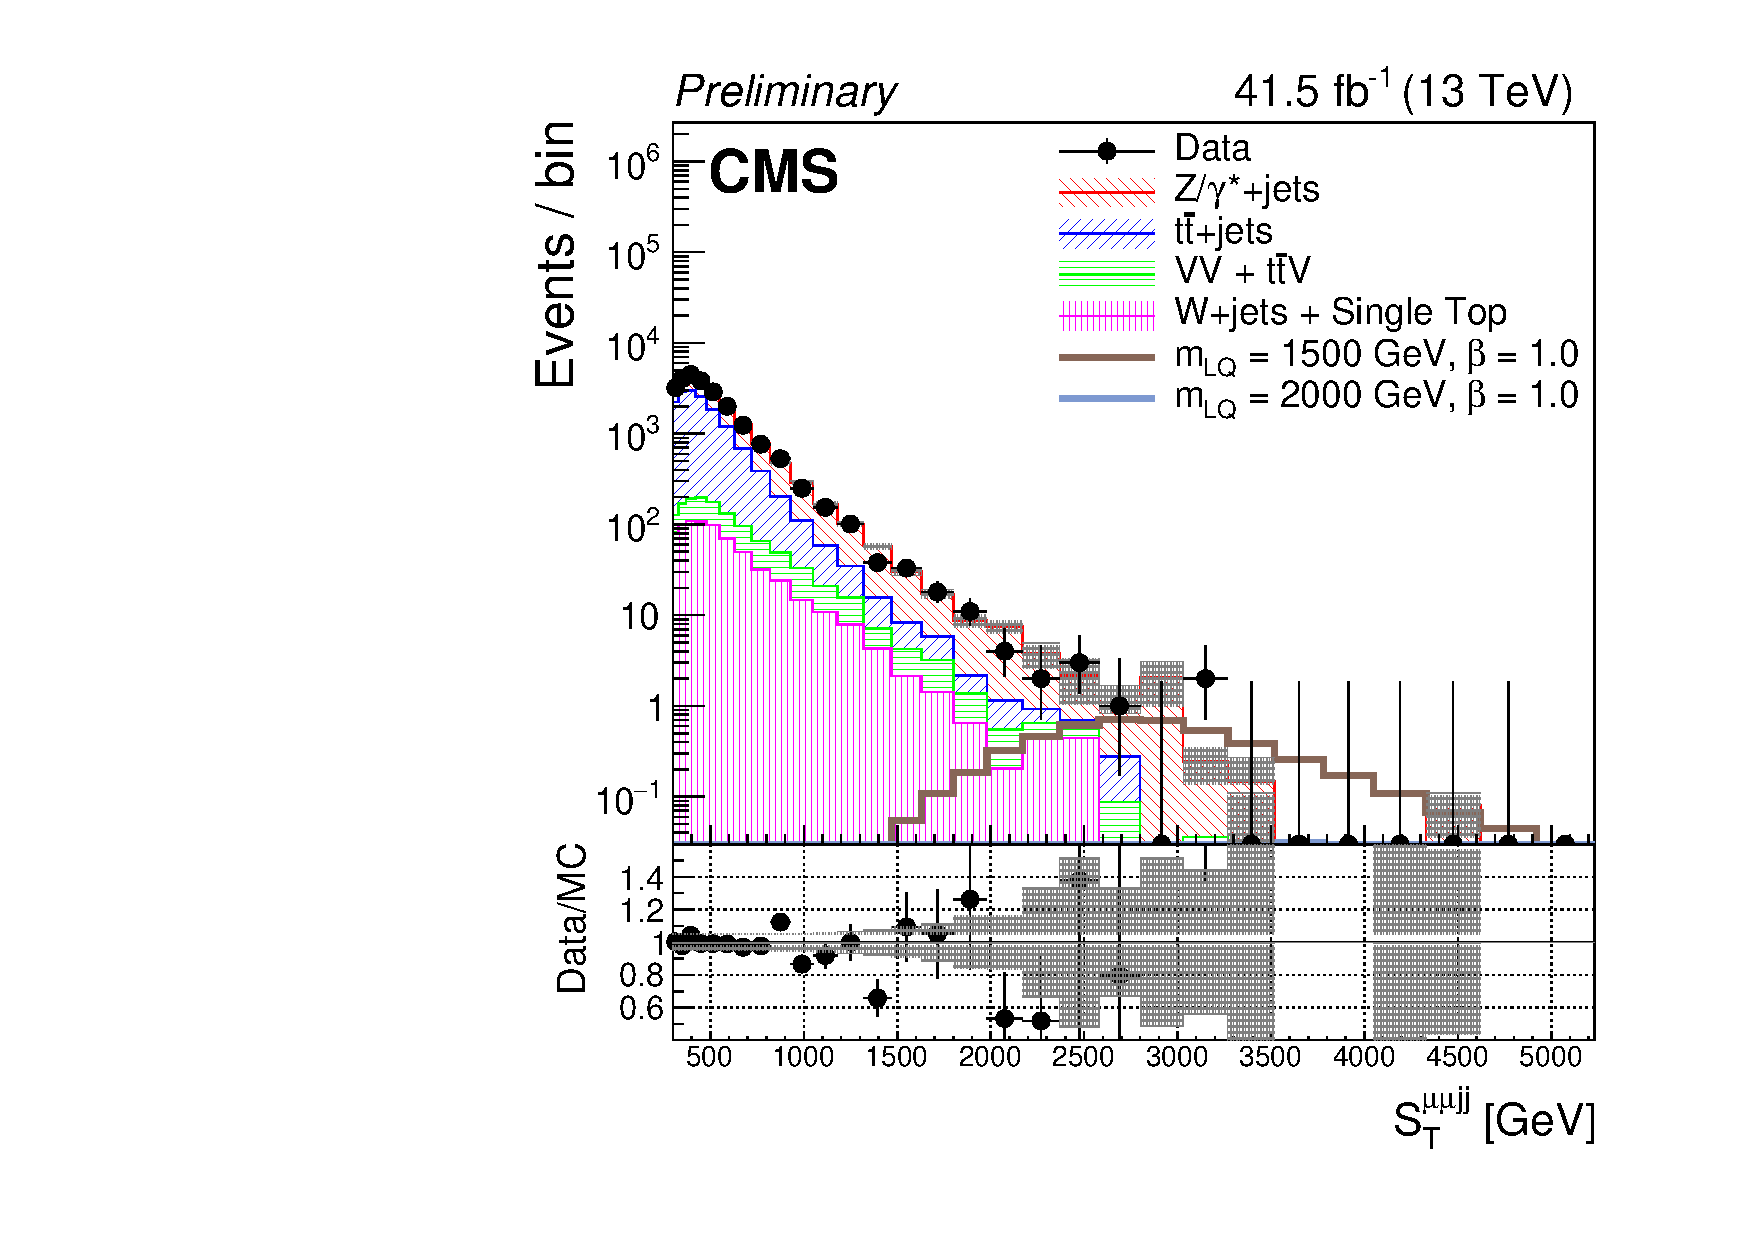
\includegraphics[width=.32\textwidth]{Images/Analysis/Results_2017_Unblinded/Plots/Preselection/BasicLQ_uujj_St_uujj_standard.pdf}}
       {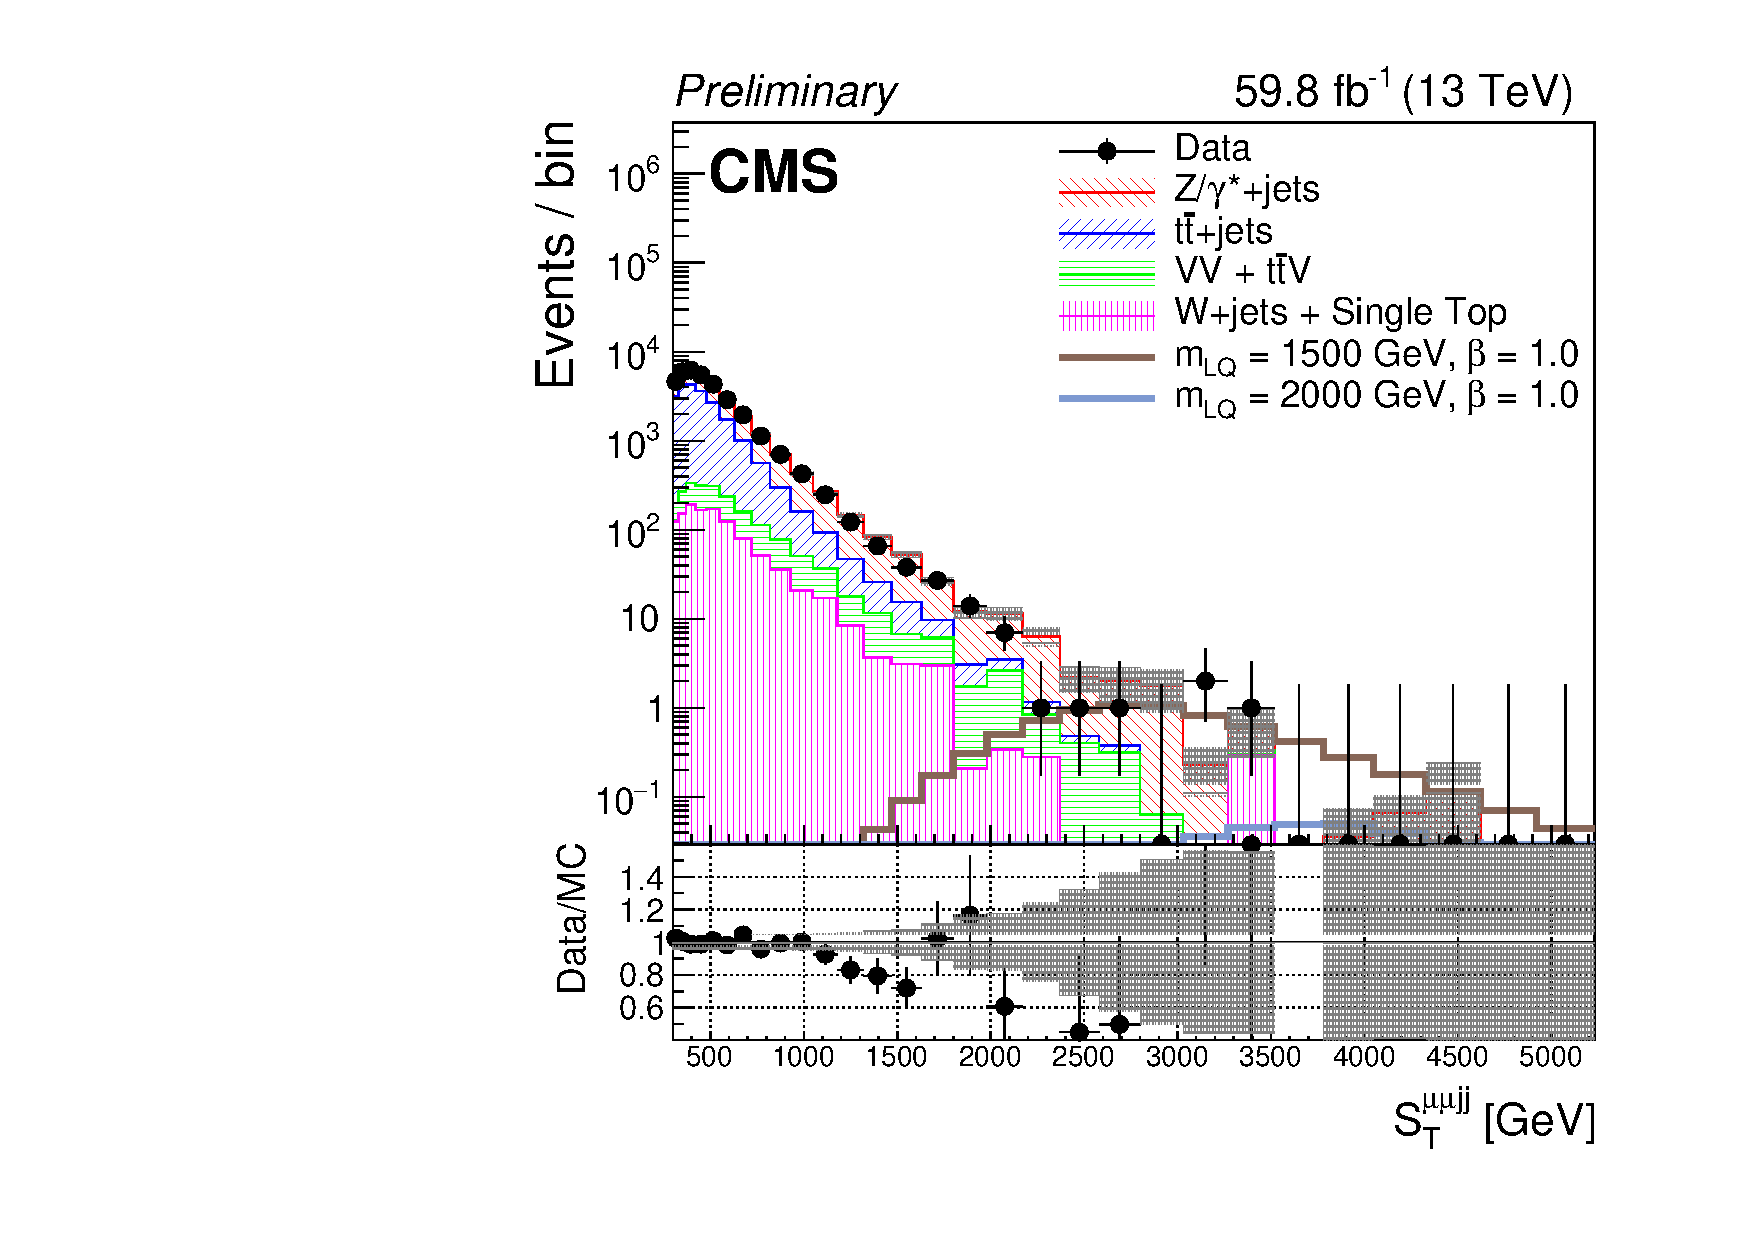
\includegraphics[width=.32\textwidth]{Images/Analysis/Results_2018_Unblinded/Plots/Preselection/BasicLQ_uujj_St_uujj_standard.pdf}}
       {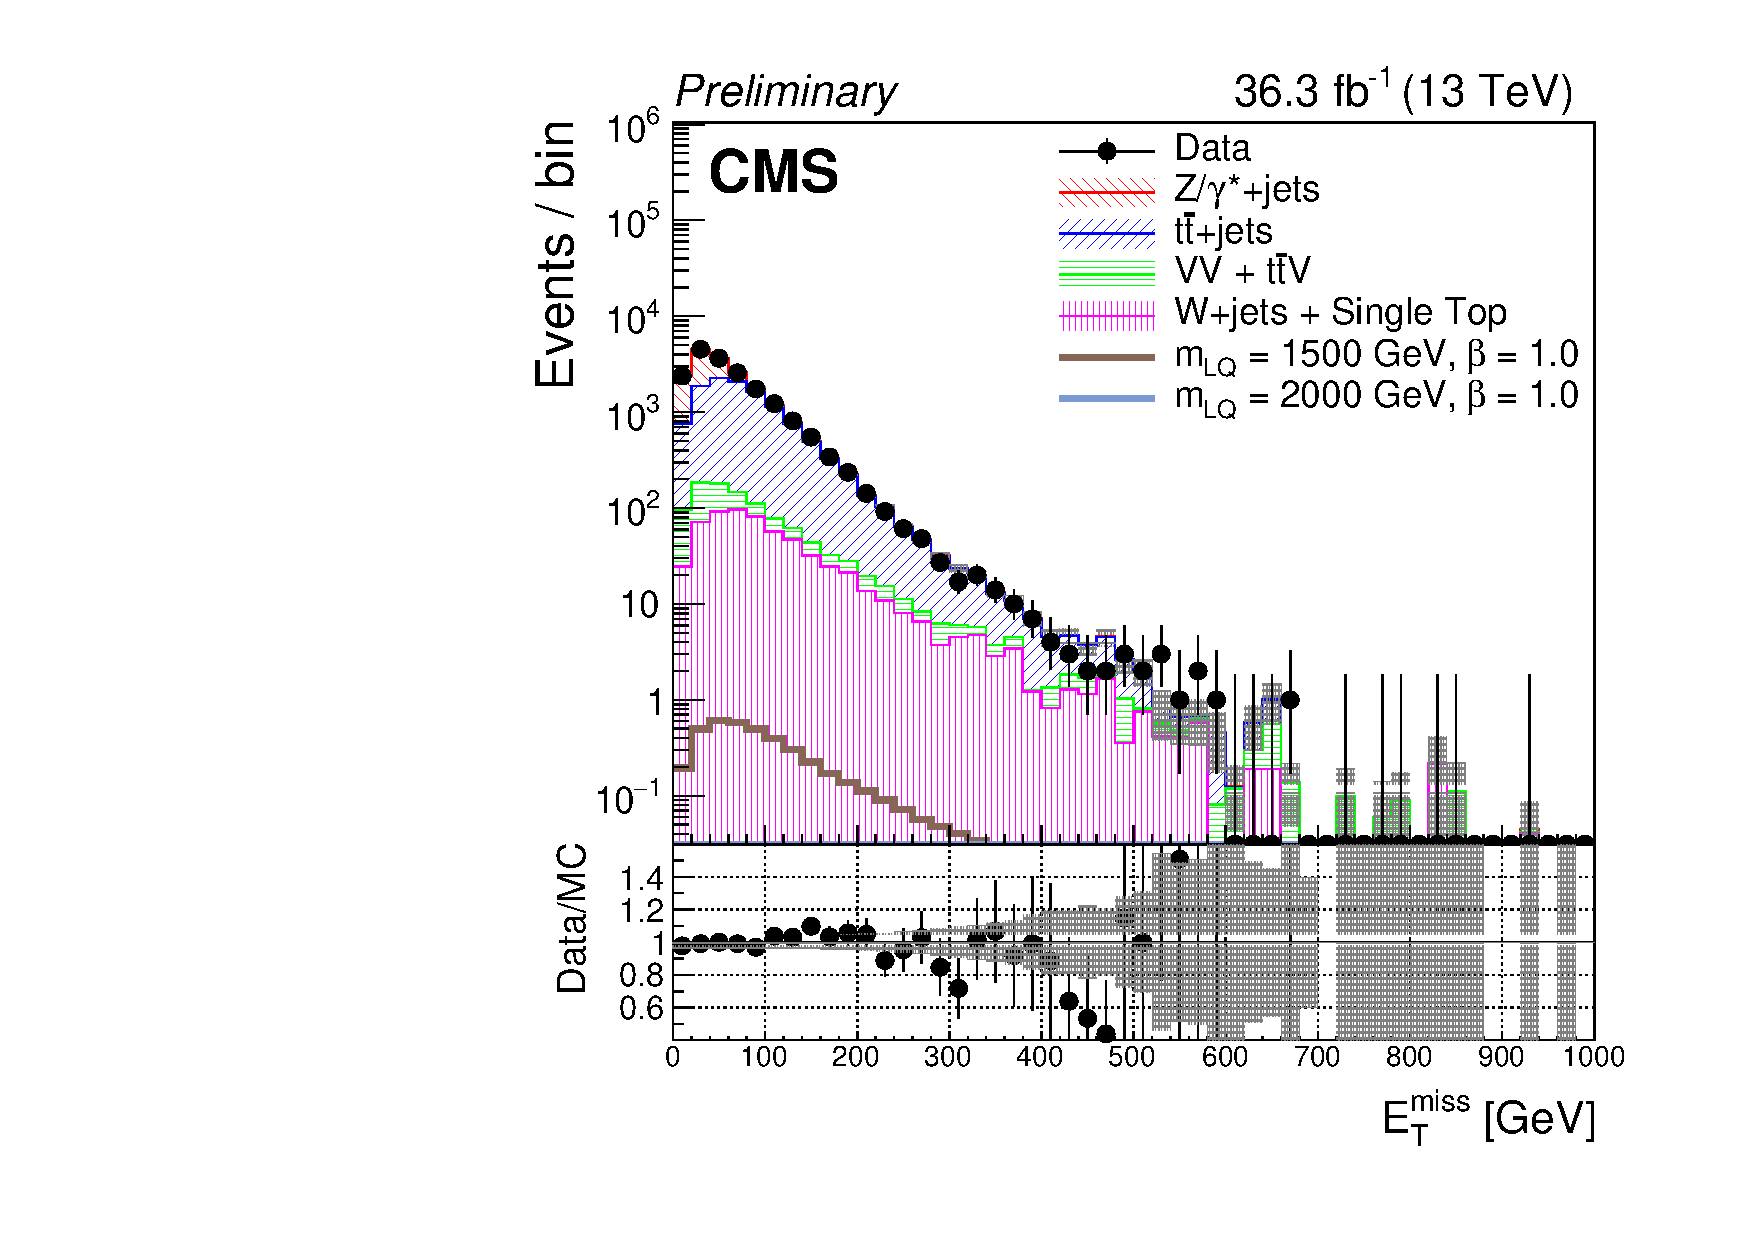
\includegraphics[width=.32\textwidth]{Images/Analysis/Results_2016_Unblinded/Plots/Preselection/BasicLQ_uujj_Pt_miss_standard.pdf}}
       {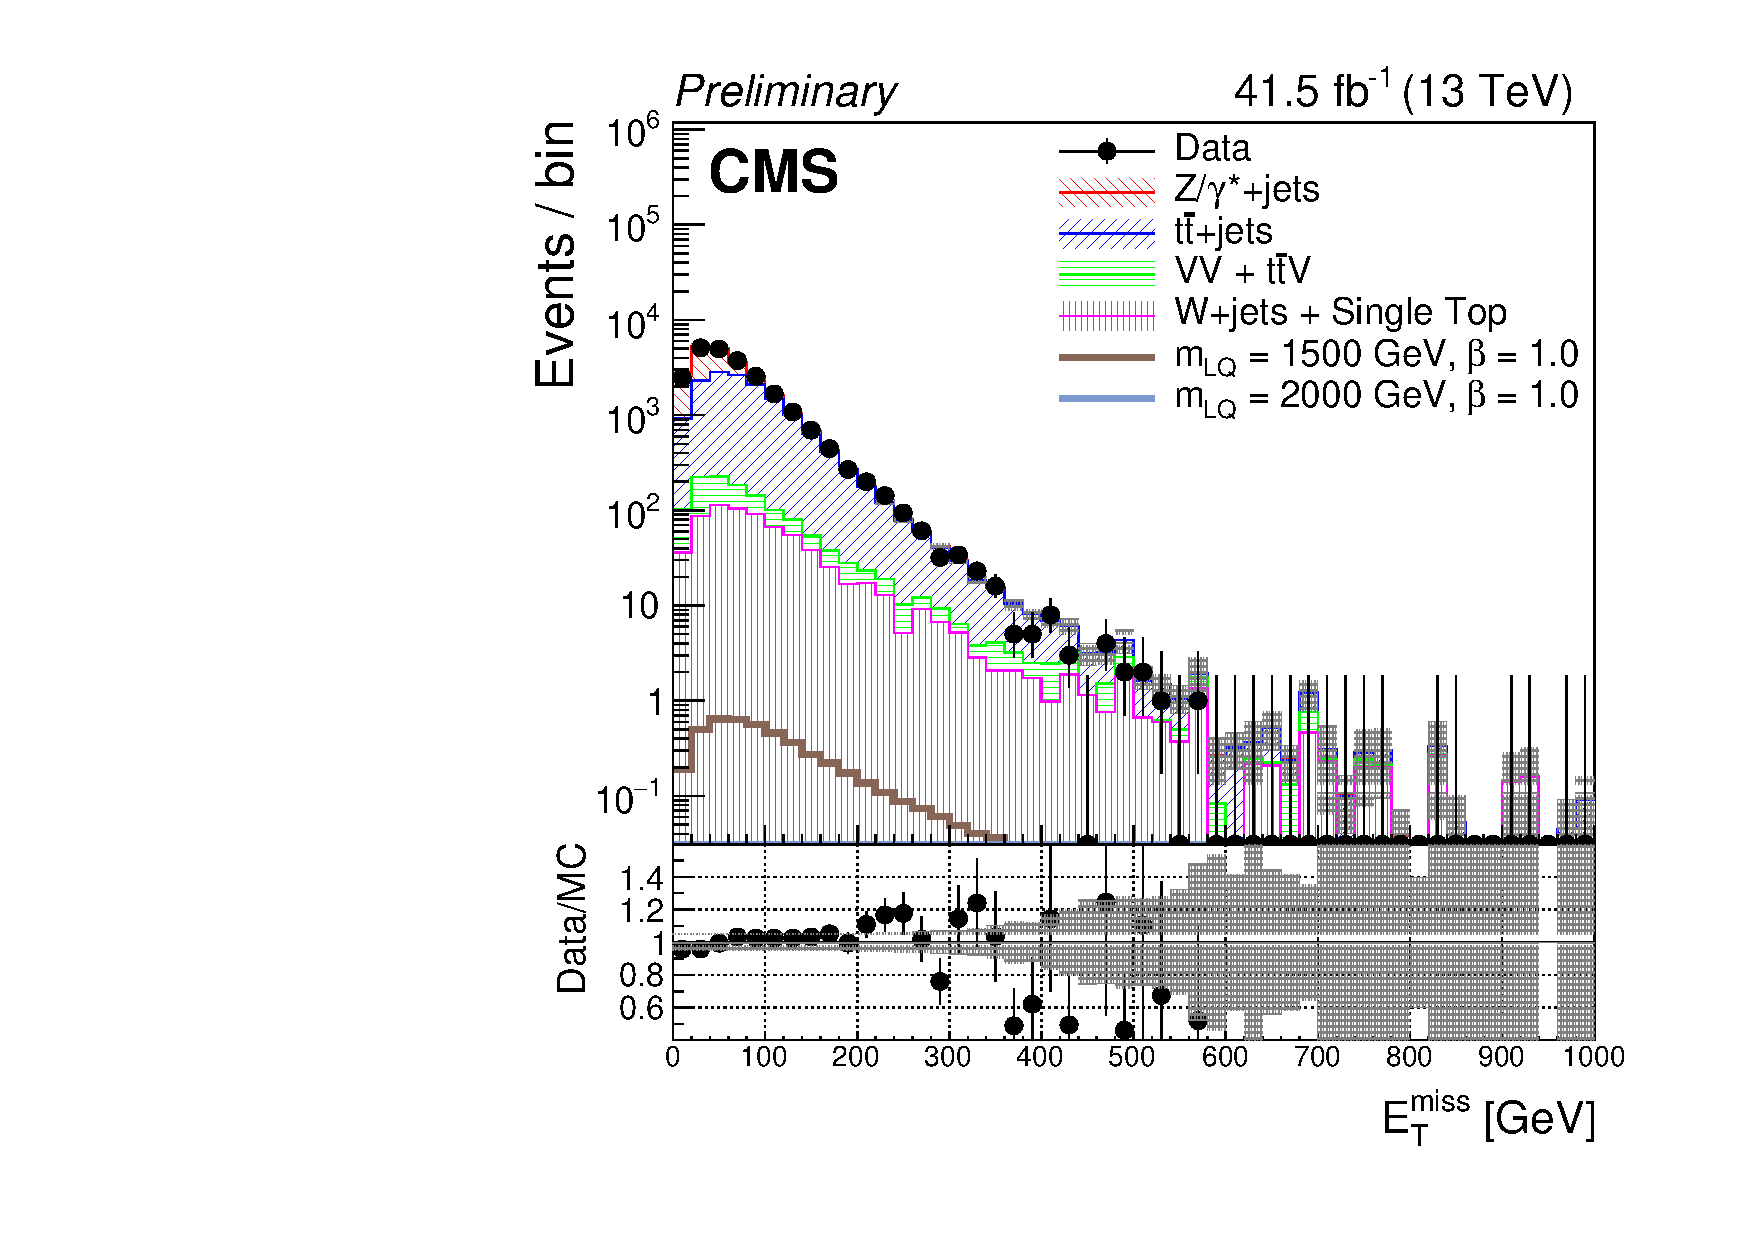
\includegraphics[width=.32\textwidth]{Images/Analysis/Results_2017_Unblinded/Plots/Preselection/BasicLQ_uujj_Pt_miss_standard.pdf}}
       {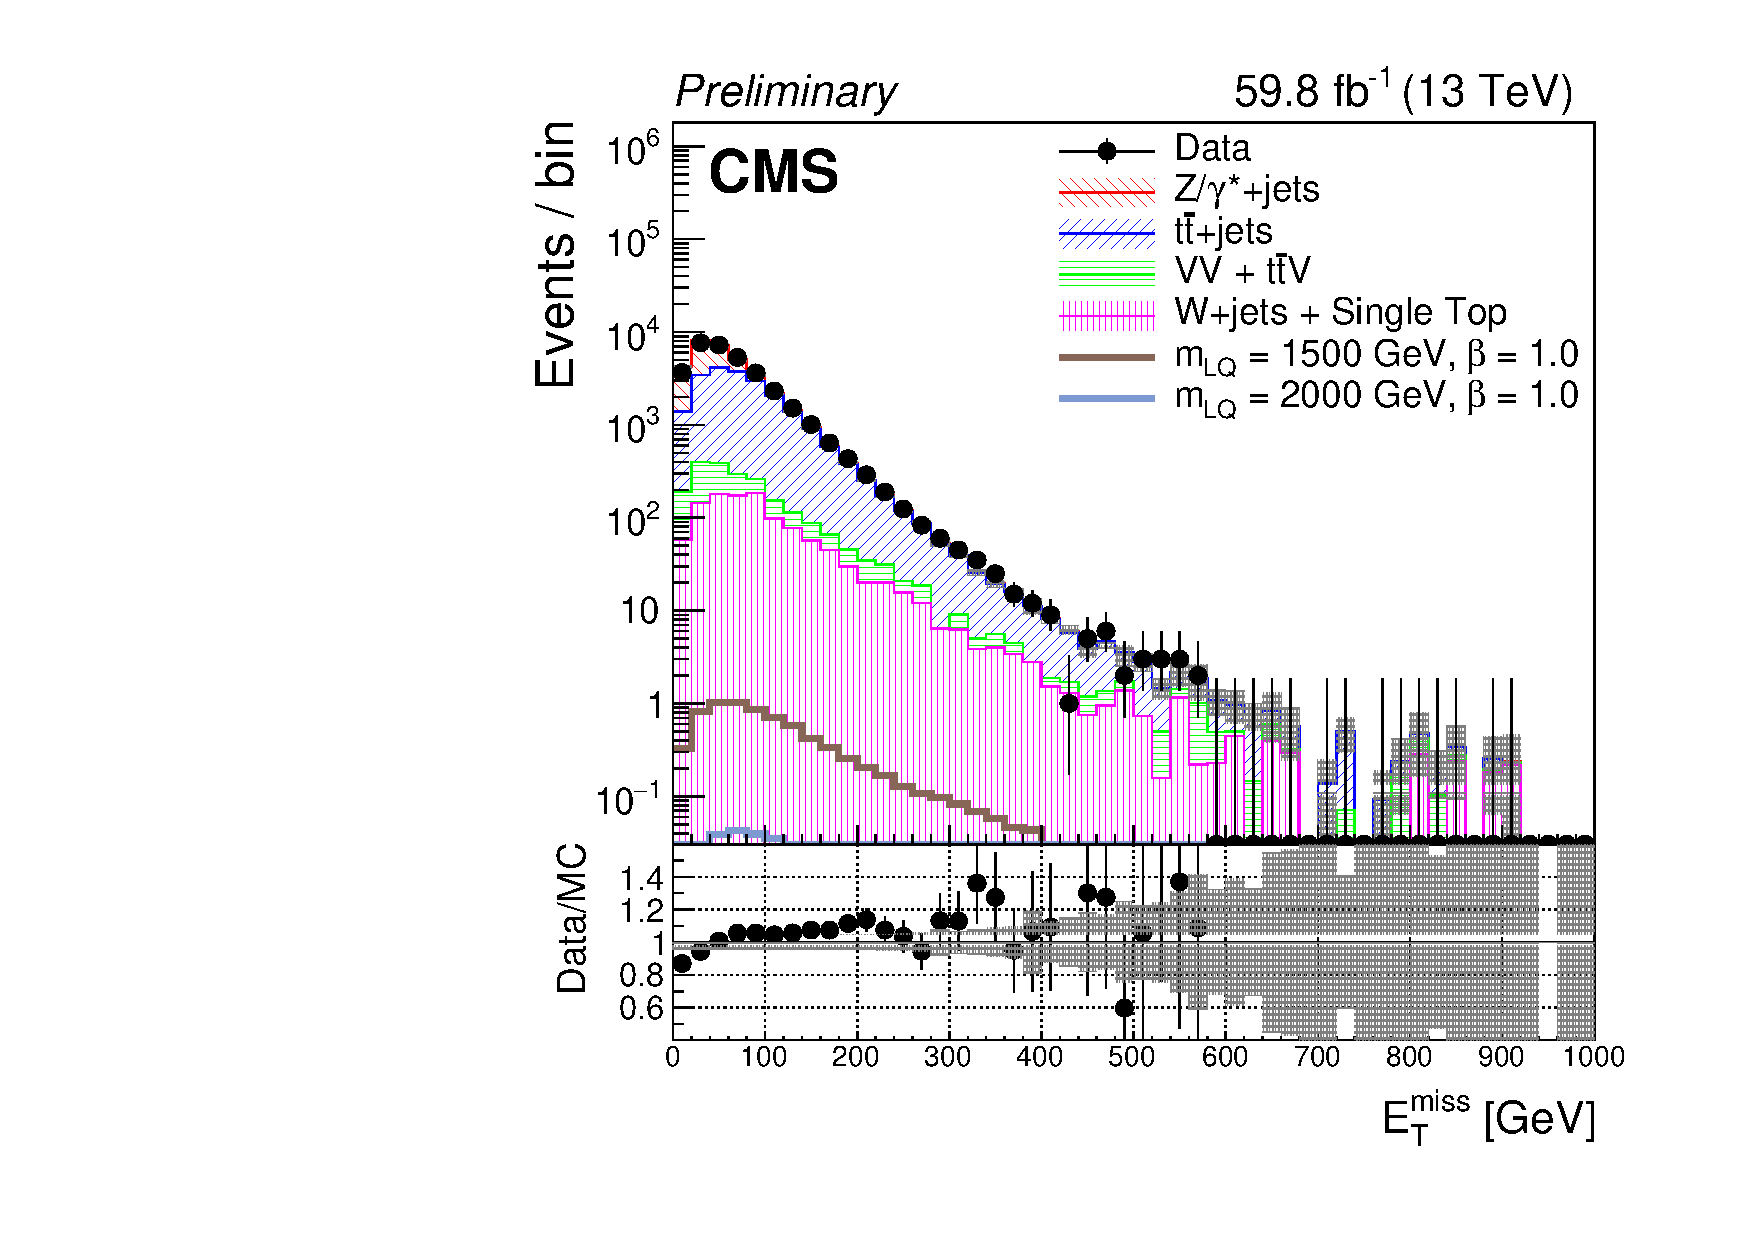
\includegraphics[width=.32\textwidth]{Images/Analysis/Results_2018_Unblinded/Plots/Preselection/BasicLQ_uujj_Pt_miss_standard.pdf}}
       {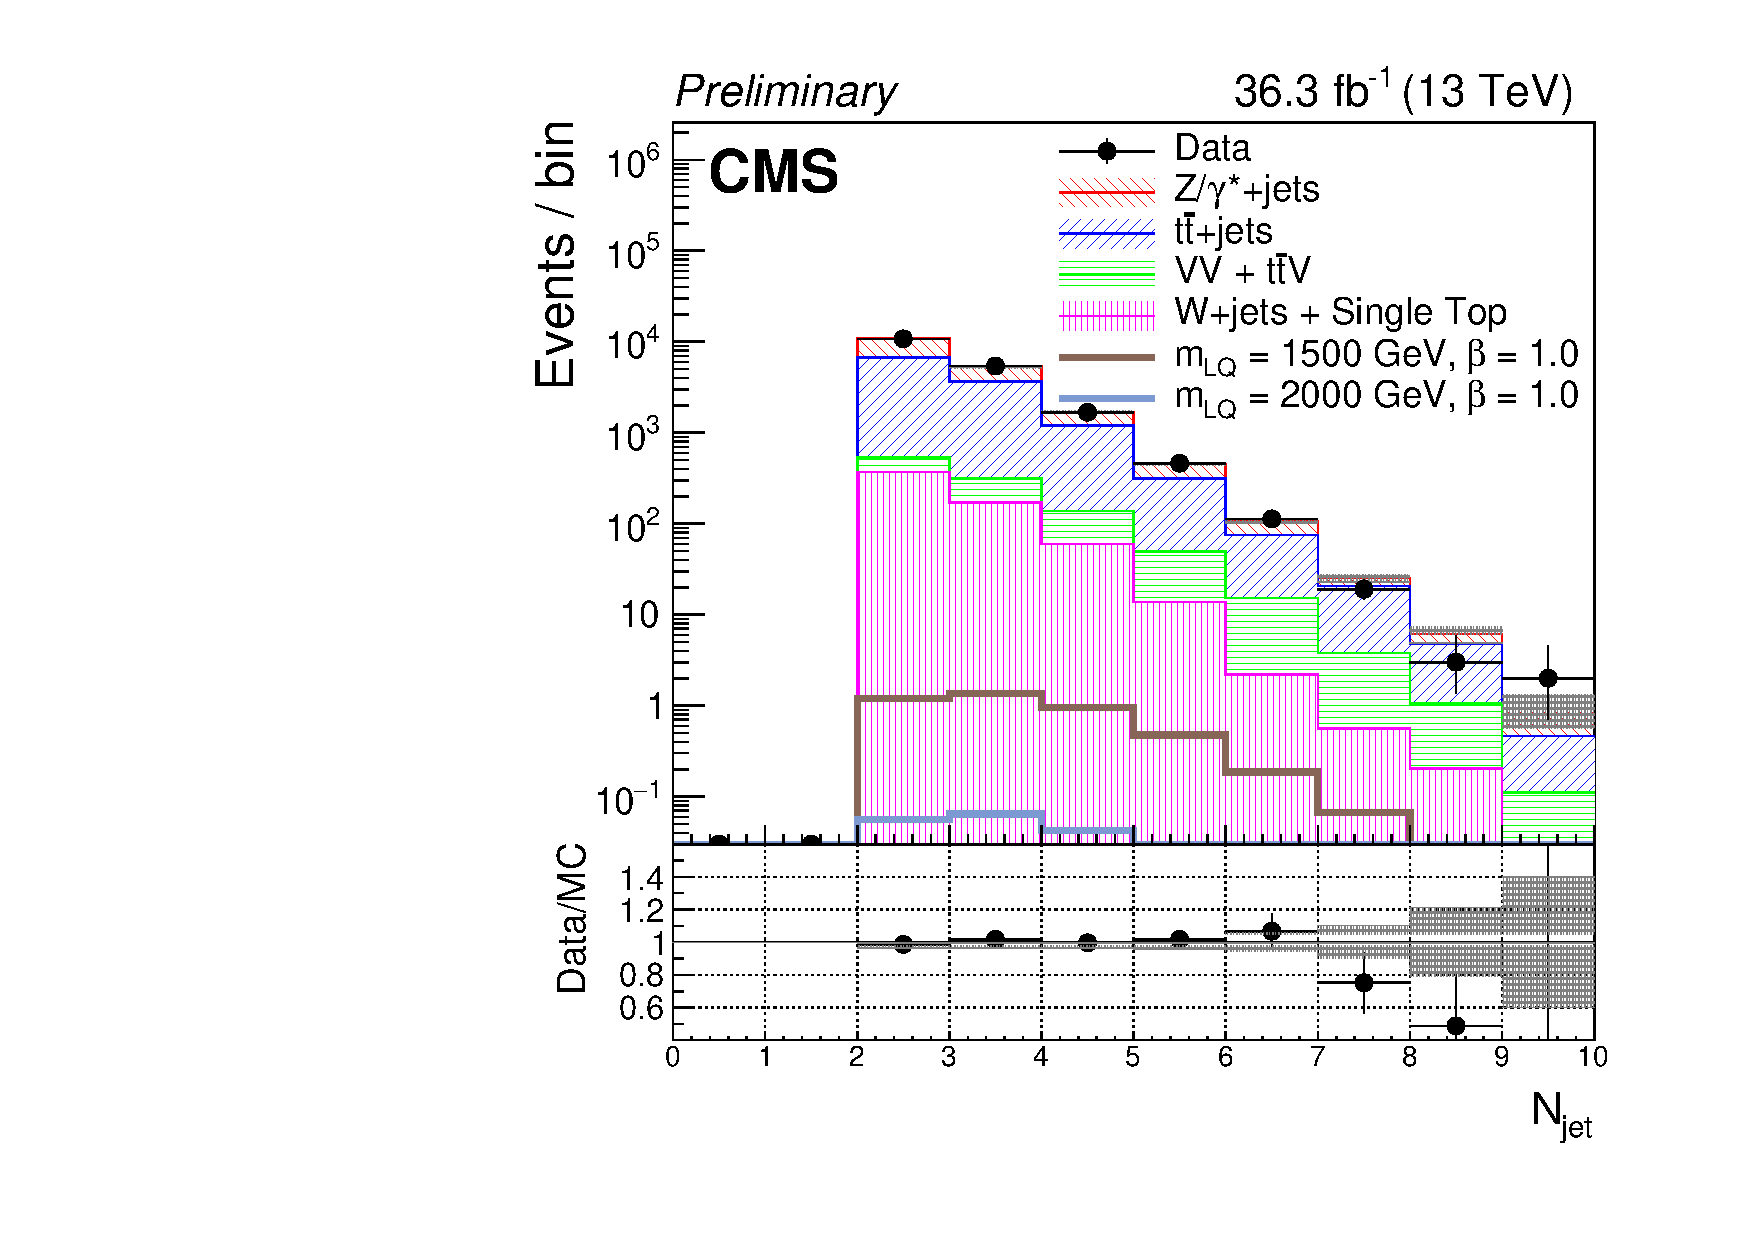
\includegraphics[width=.32\textwidth]{Images/Analysis/Results_2016_Unblinded/Plots/Preselection/BasicLQ_uujj_JetCount_standard.pdf}}
       {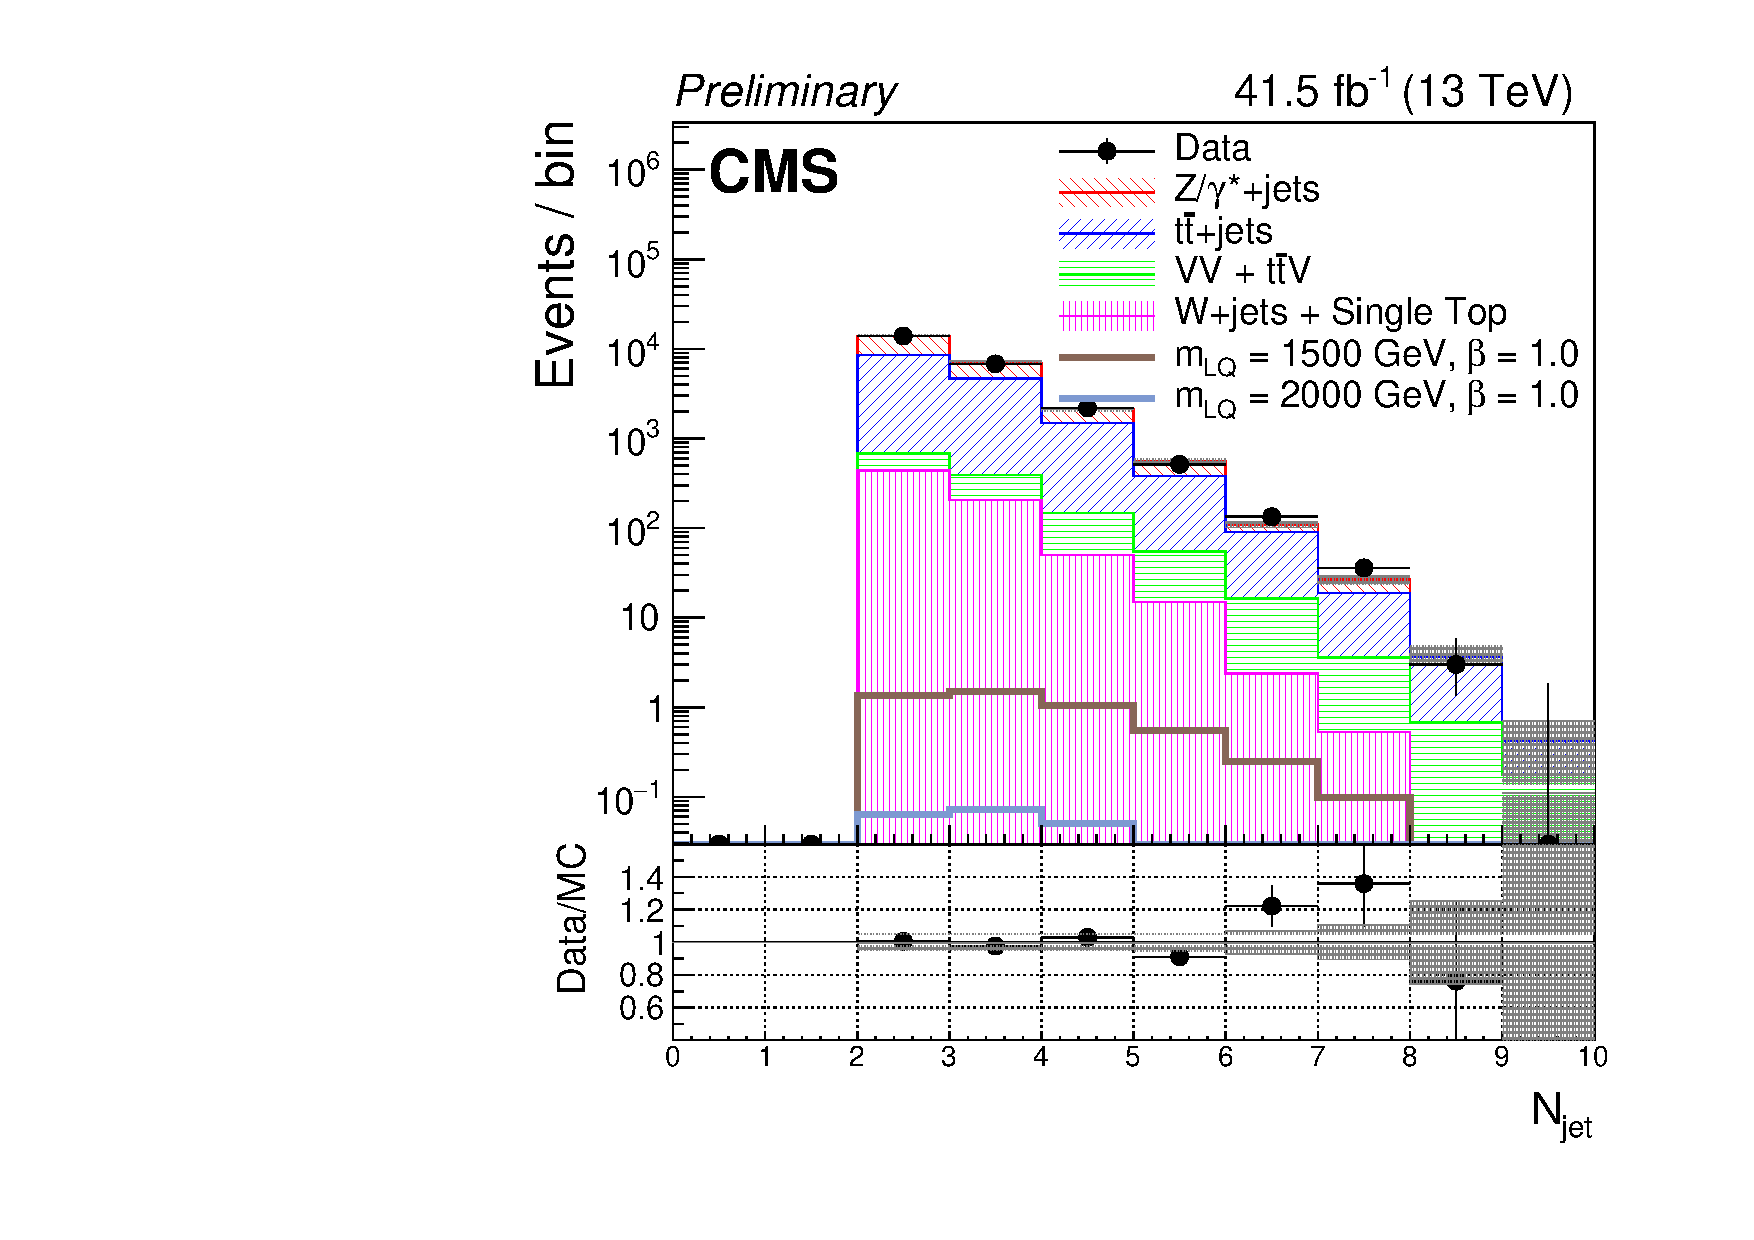
\includegraphics[width=.32\textwidth]{Images/Analysis/Results_2017_Unblinded/Plots/Preselection/BasicLQ_uujj_JetCount_standard.pdf}}
       {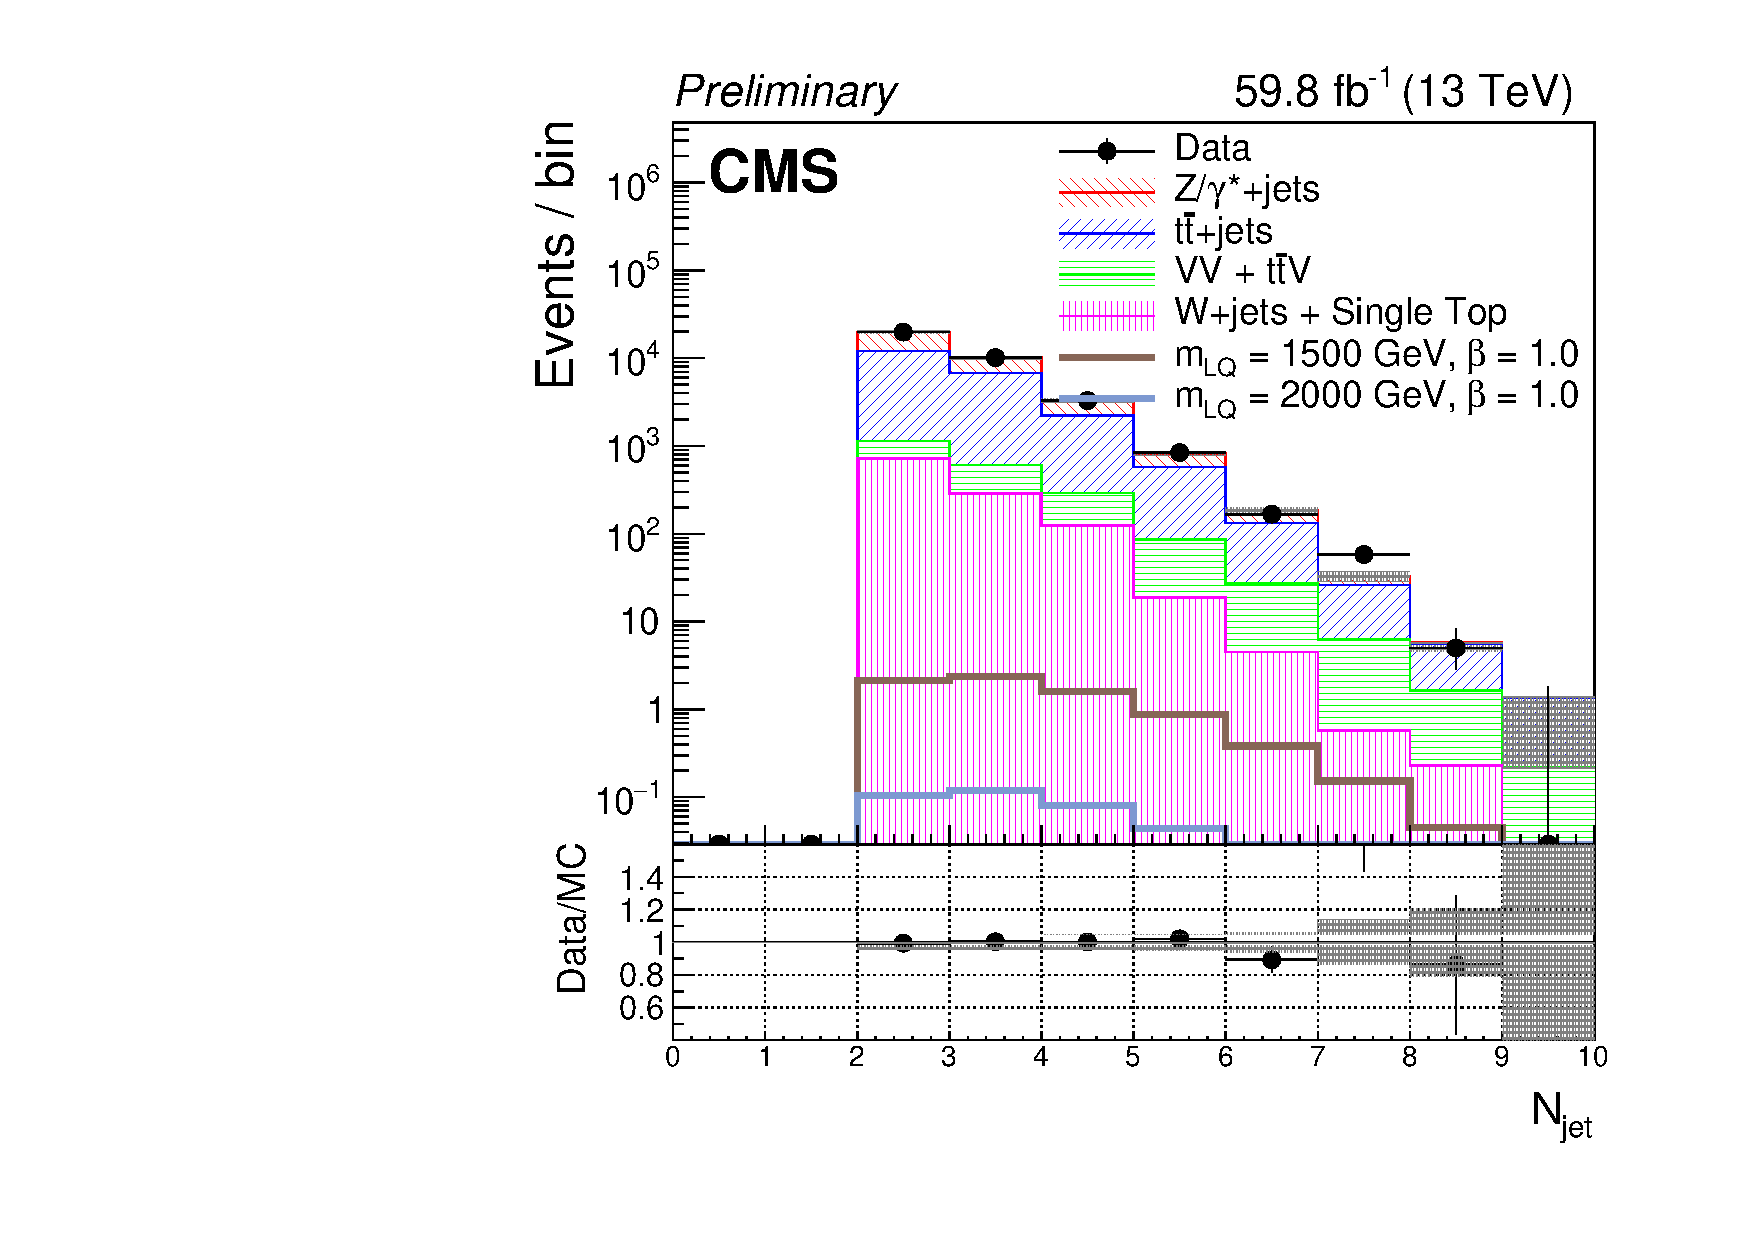
\includegraphics[width=.32\textwidth]{Images/Analysis/Results_2018_Unblinded/Plots/Preselection/BasicLQ_uujj_JetCount_standard.pdf}}
       {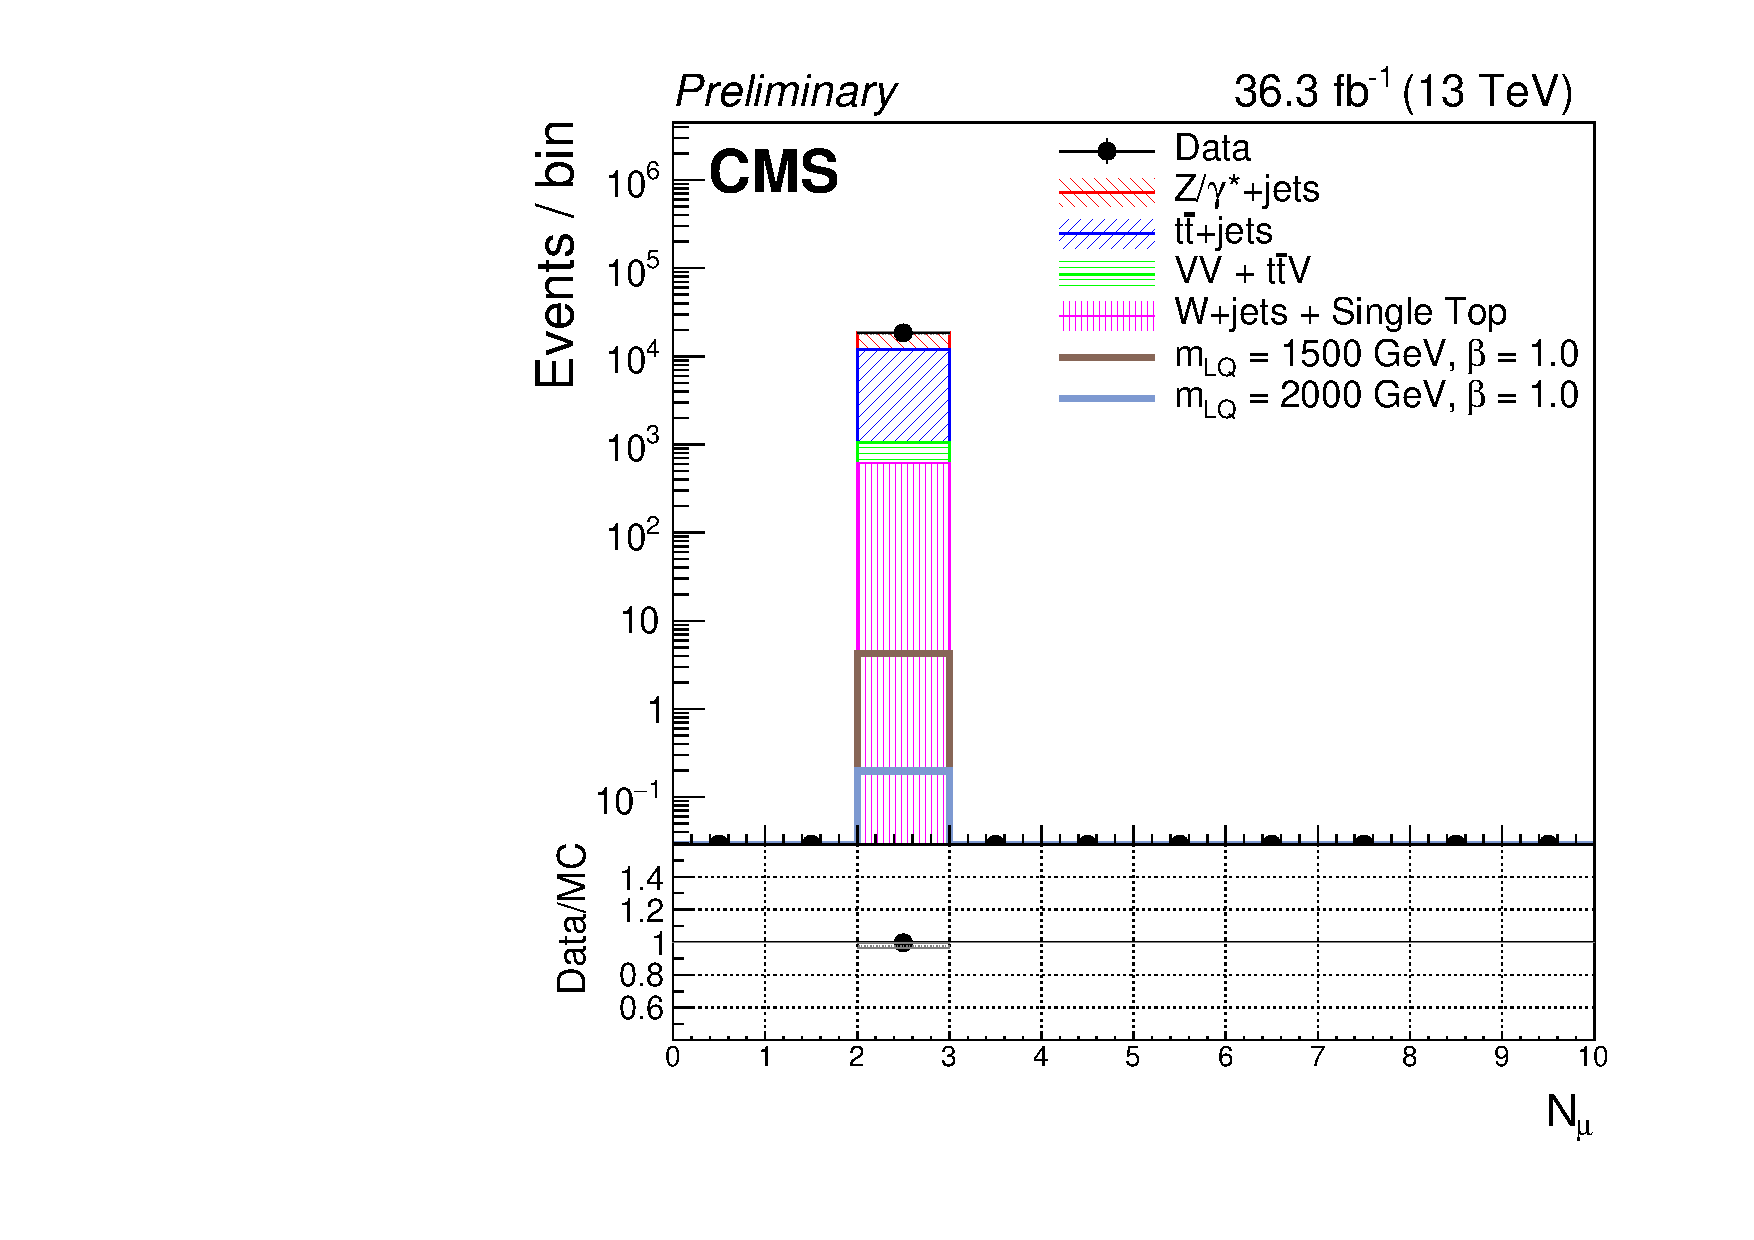
\includegraphics[width=.32\textwidth]{Images/Analysis/Results_2016_Unblinded/Plots/Preselection/BasicLQ_uujj_MuonCount_standard.pdf}}
       {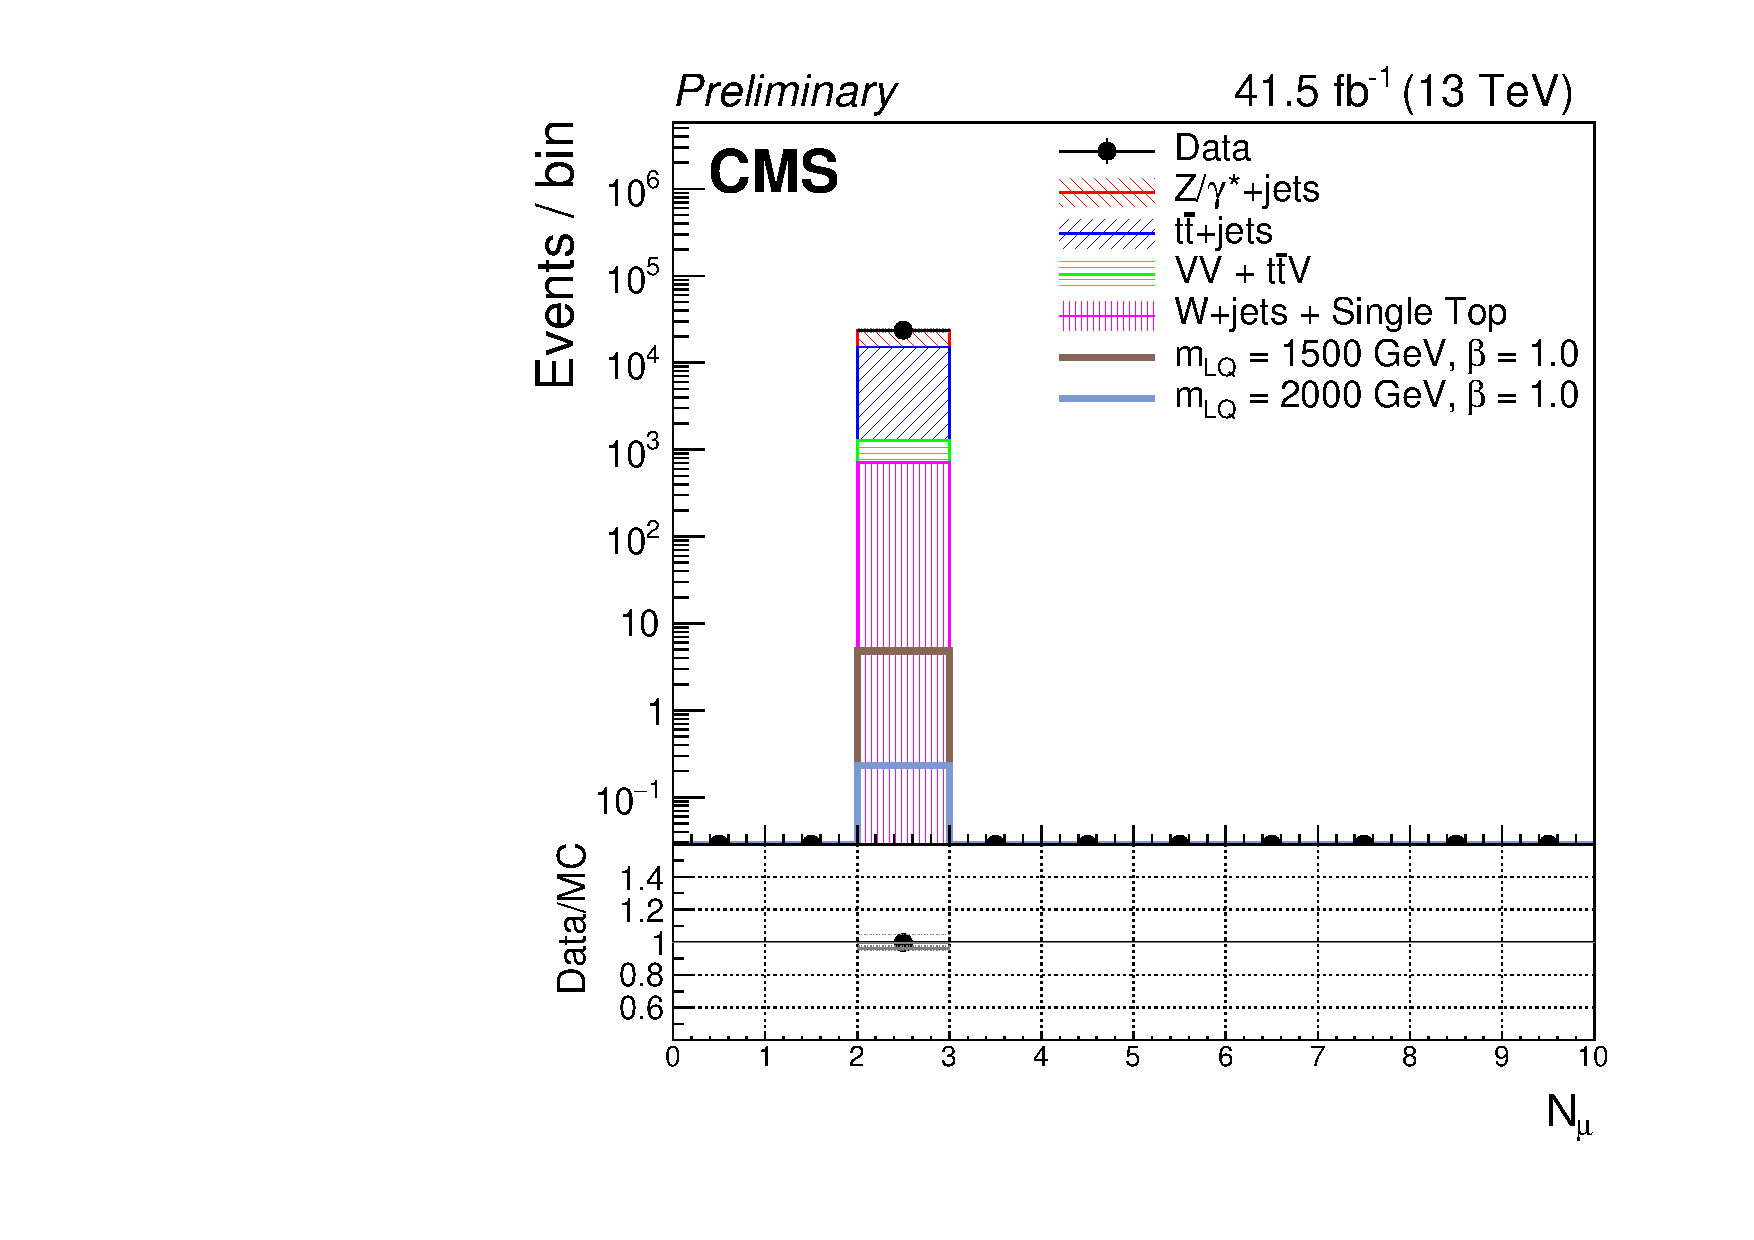
\includegraphics[width=.32\textwidth]{Images/Analysis/Results_2017_Unblinded/Plots/Preselection/BasicLQ_uujj_MuonCount_standard.pdf}}
       {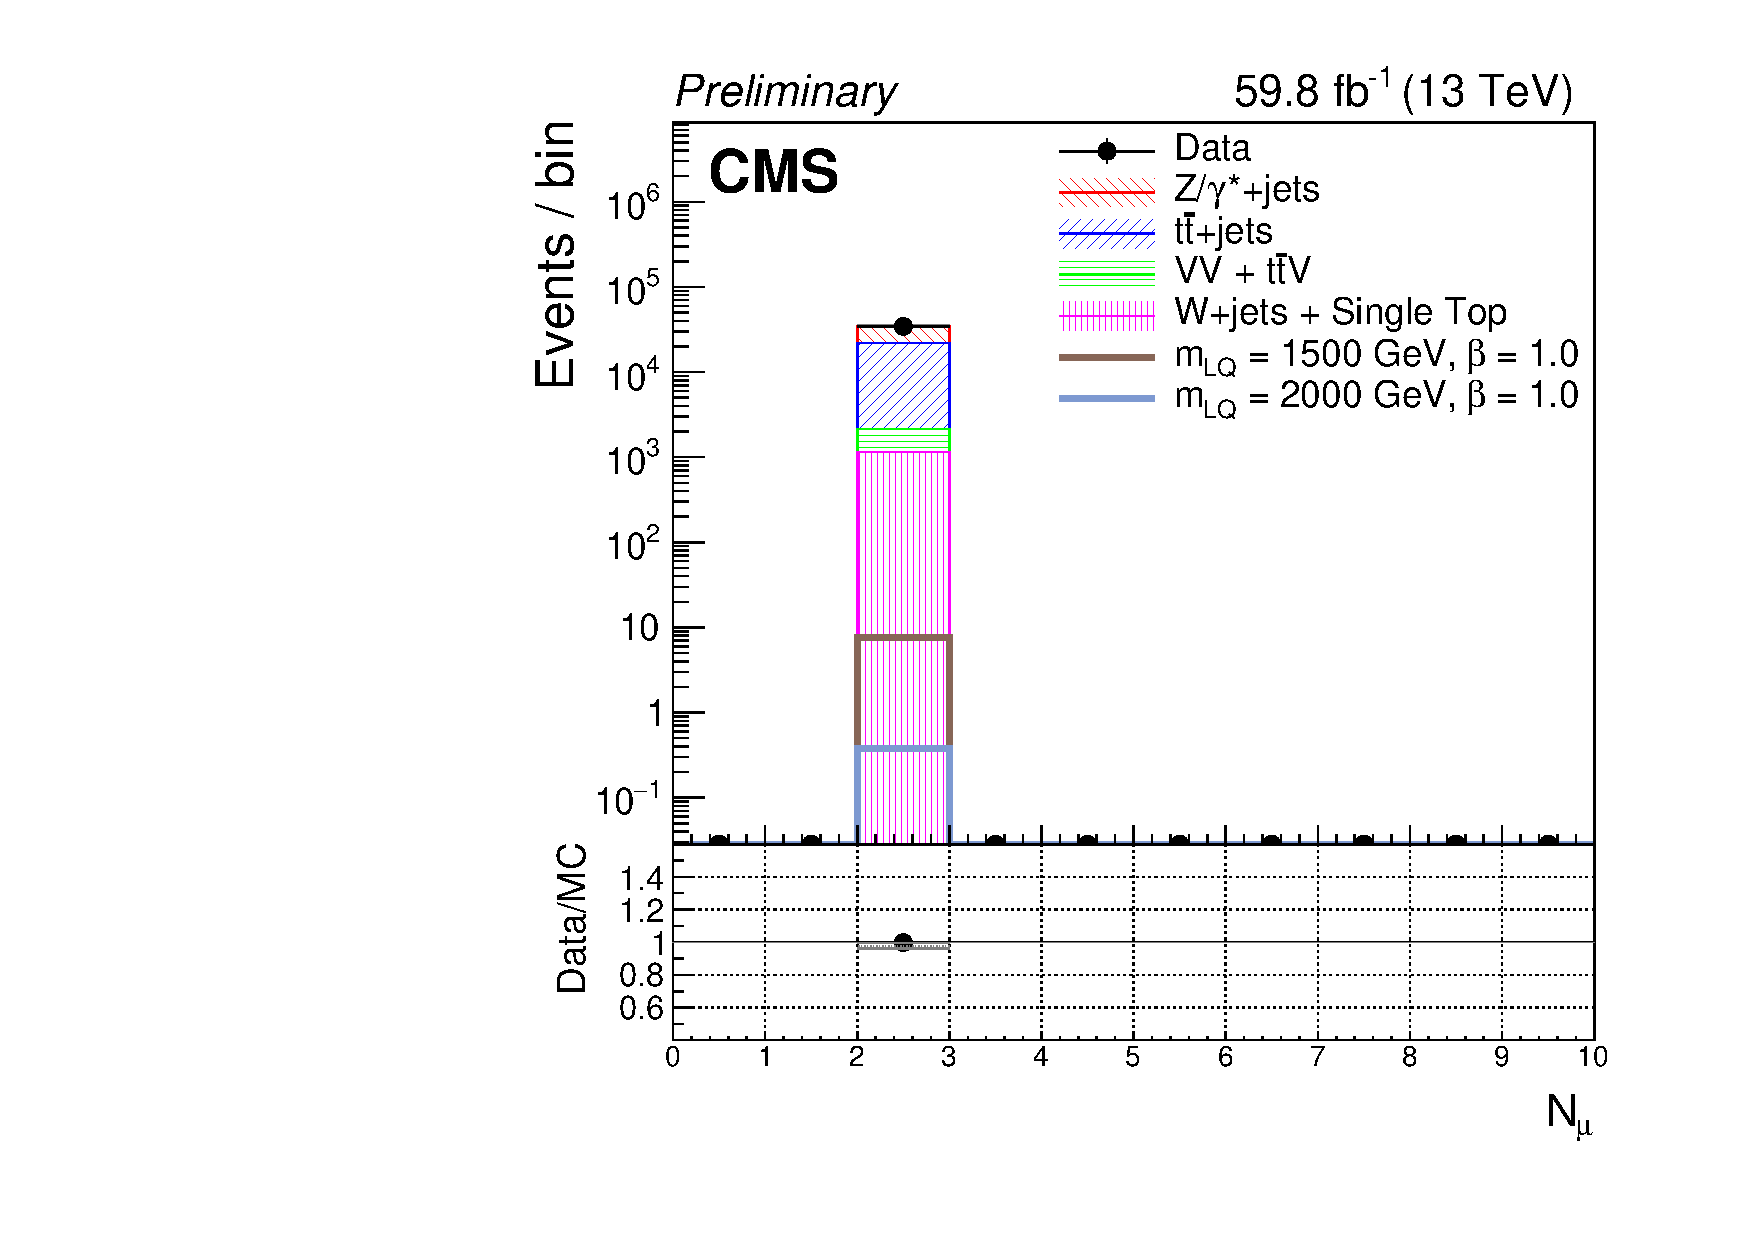
\includegraphics[width=.32\textwidth]{Images/Analysis/Results_2018_Unblinded/Plots/Preselection/BasicLQ_uujj_MuonCount_standard.pdf}}
       \caption{A comparison between distributions of observed data and SM expectation at preselection level. Left to right: 2016, 2017, 2018 data. Top to bottom: \ST, \ptmiss, jet multiplicity, and muon multiplicity. Error bars on observed data points represent statistical uncertainties, and systematic uncertainties on SM expectation are shown by gray hashing.}
    \label{figapp:preselmisc}
\end{figure}

\begin{figure}[H]
       \centering
       {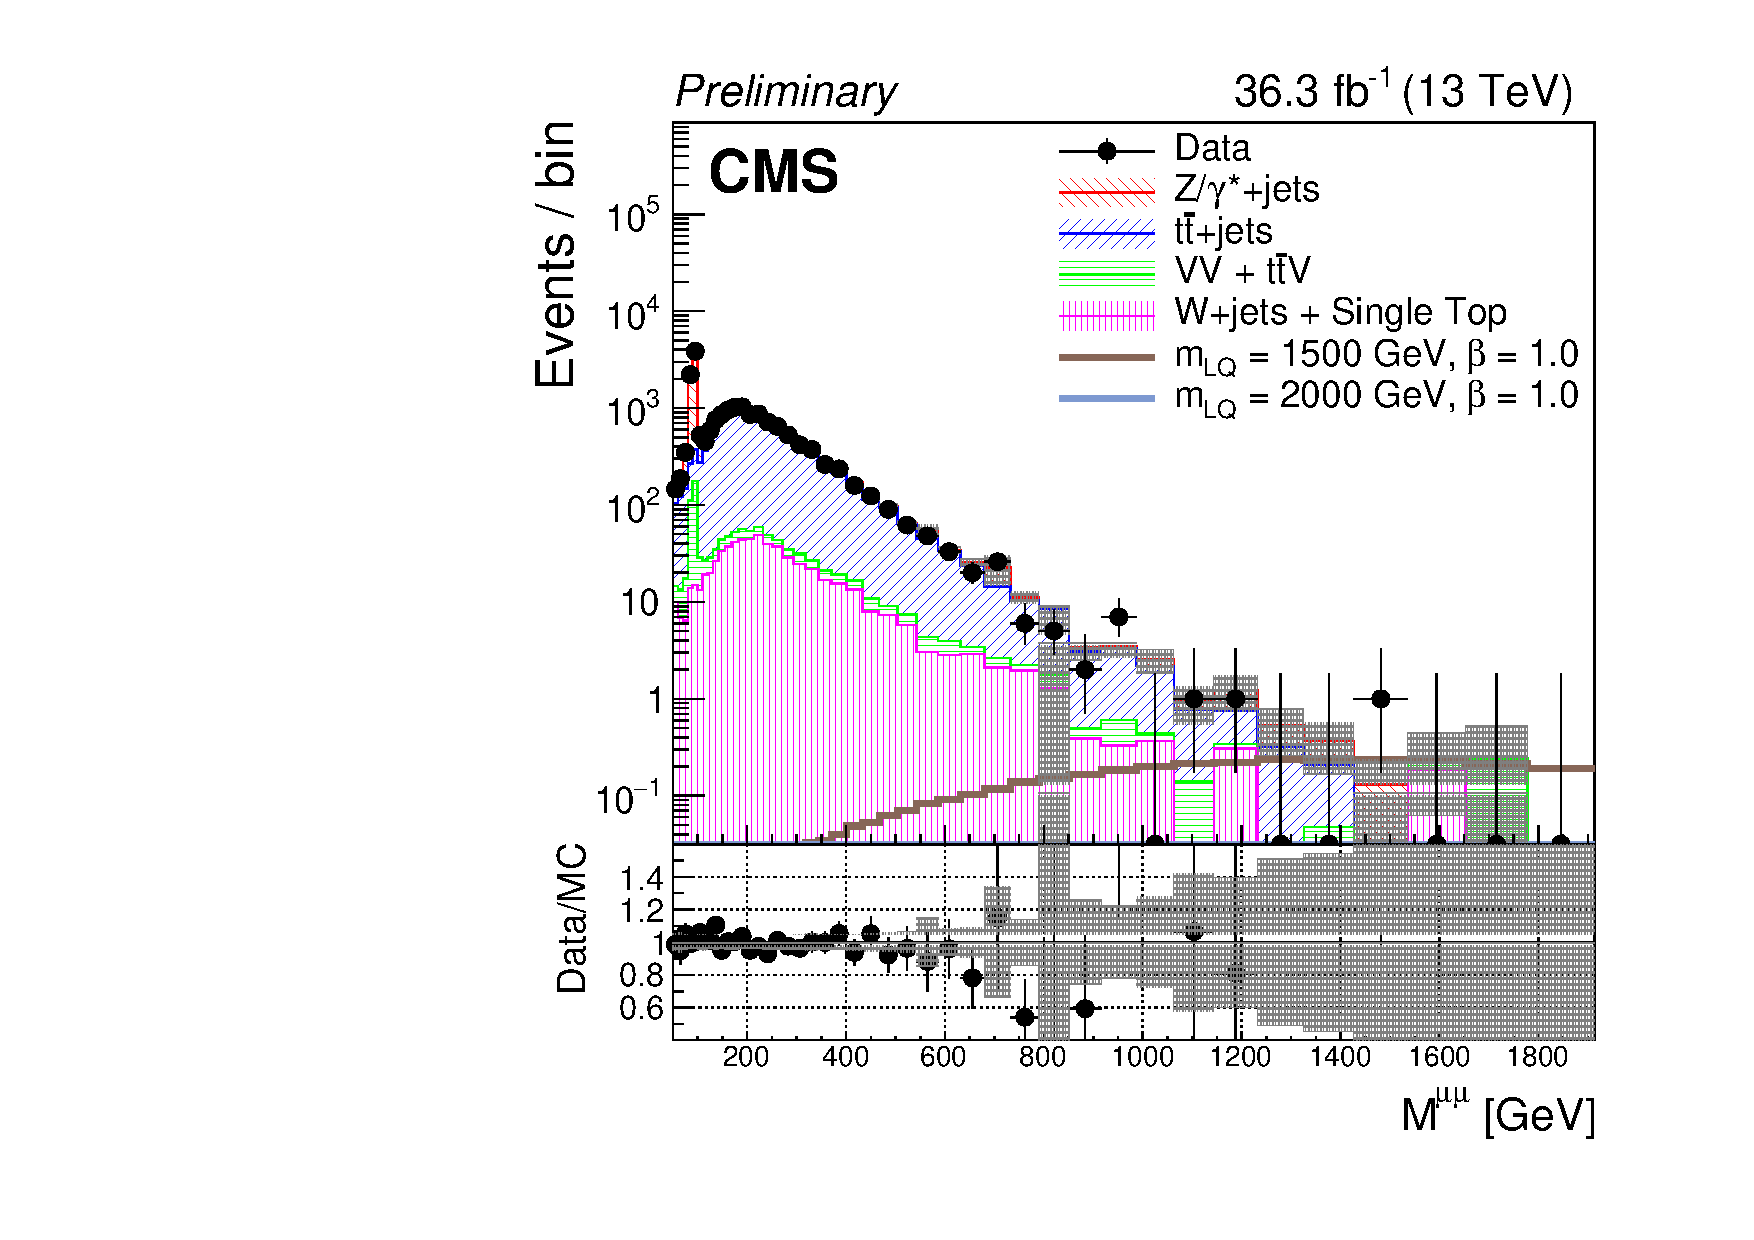
\includegraphics[width=.32\textwidth]{Images/Analysis/Results_2016_Unblinded/Plots/Preselection/BasicLQ_uujj_M_uu_standard.pdf}}
       {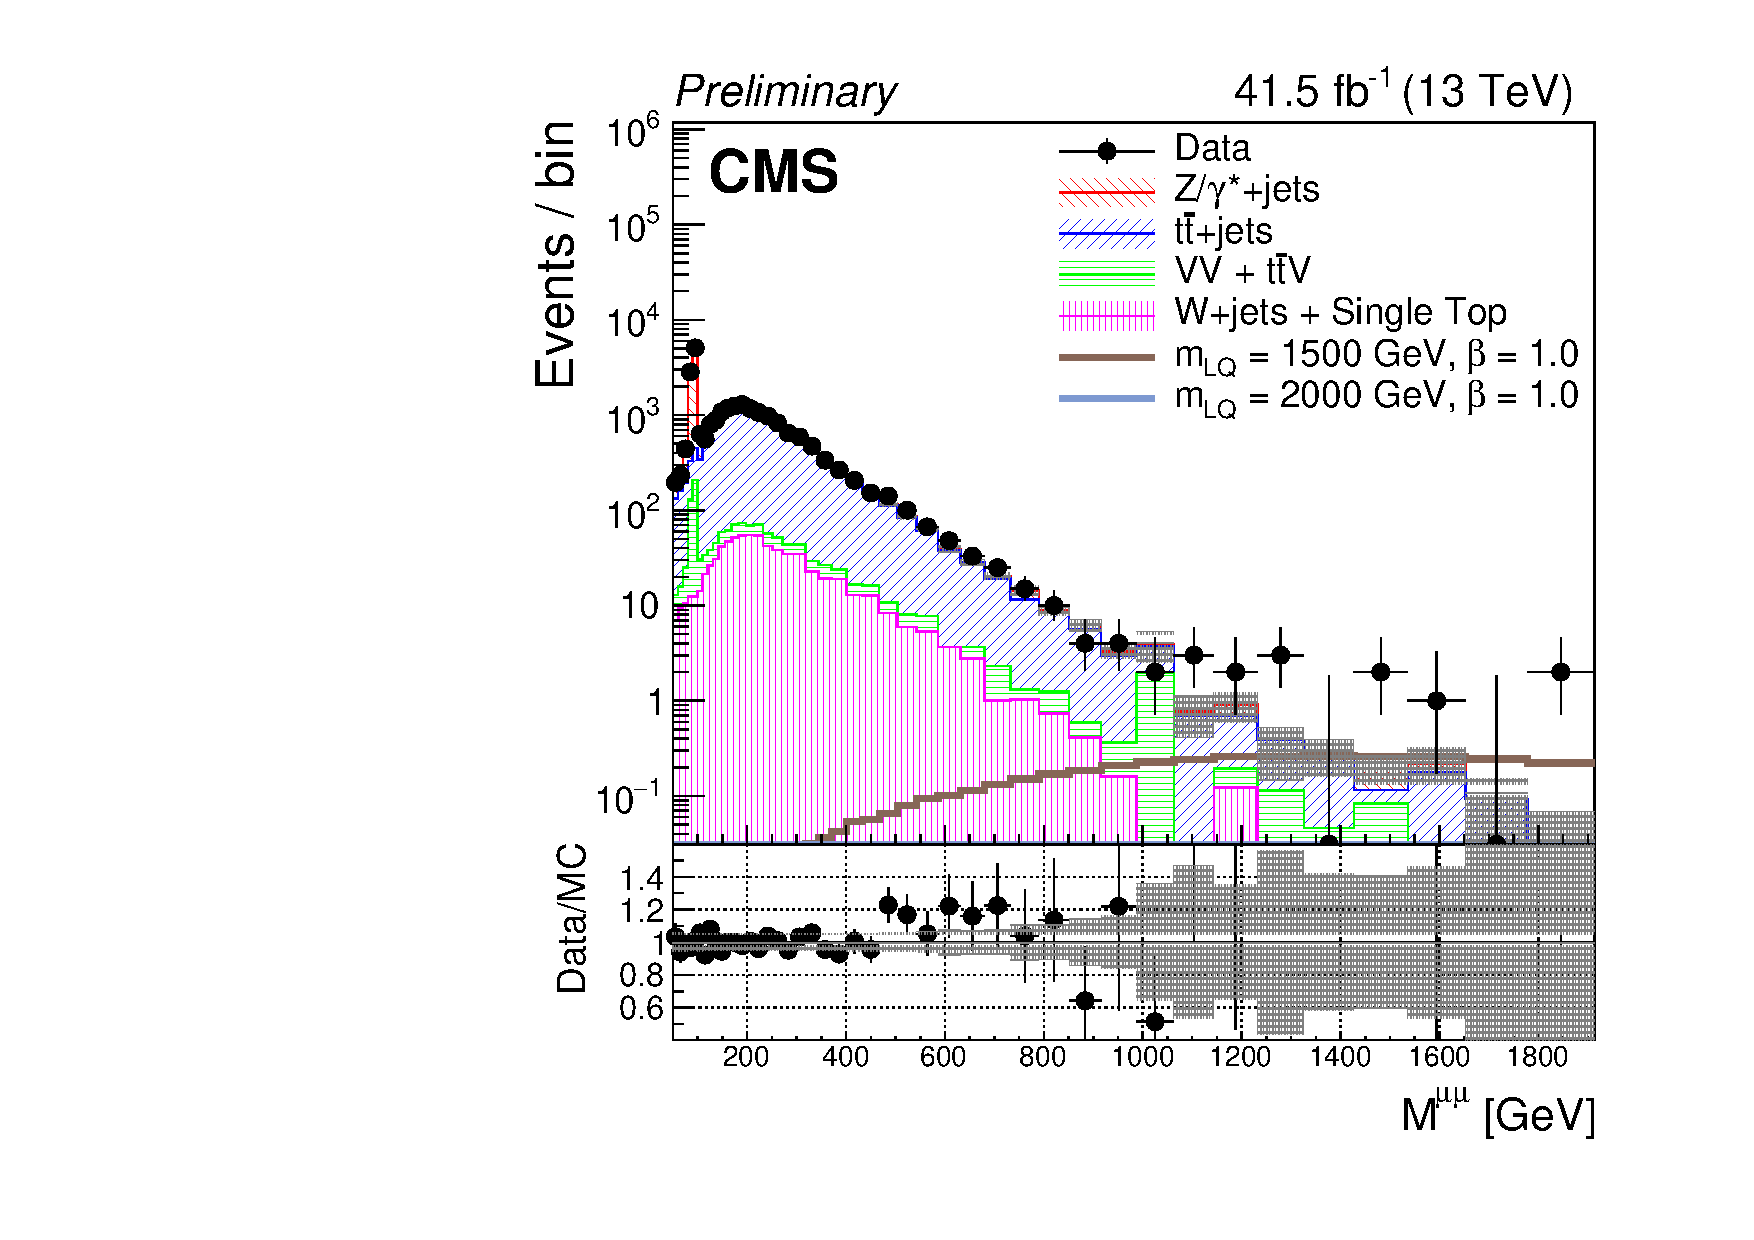
\includegraphics[width=.32\textwidth]{Images/Analysis/Results_2017_Unblinded/Plots/Preselection/BasicLQ_uujj_M_uu_standard.pdf}}
       {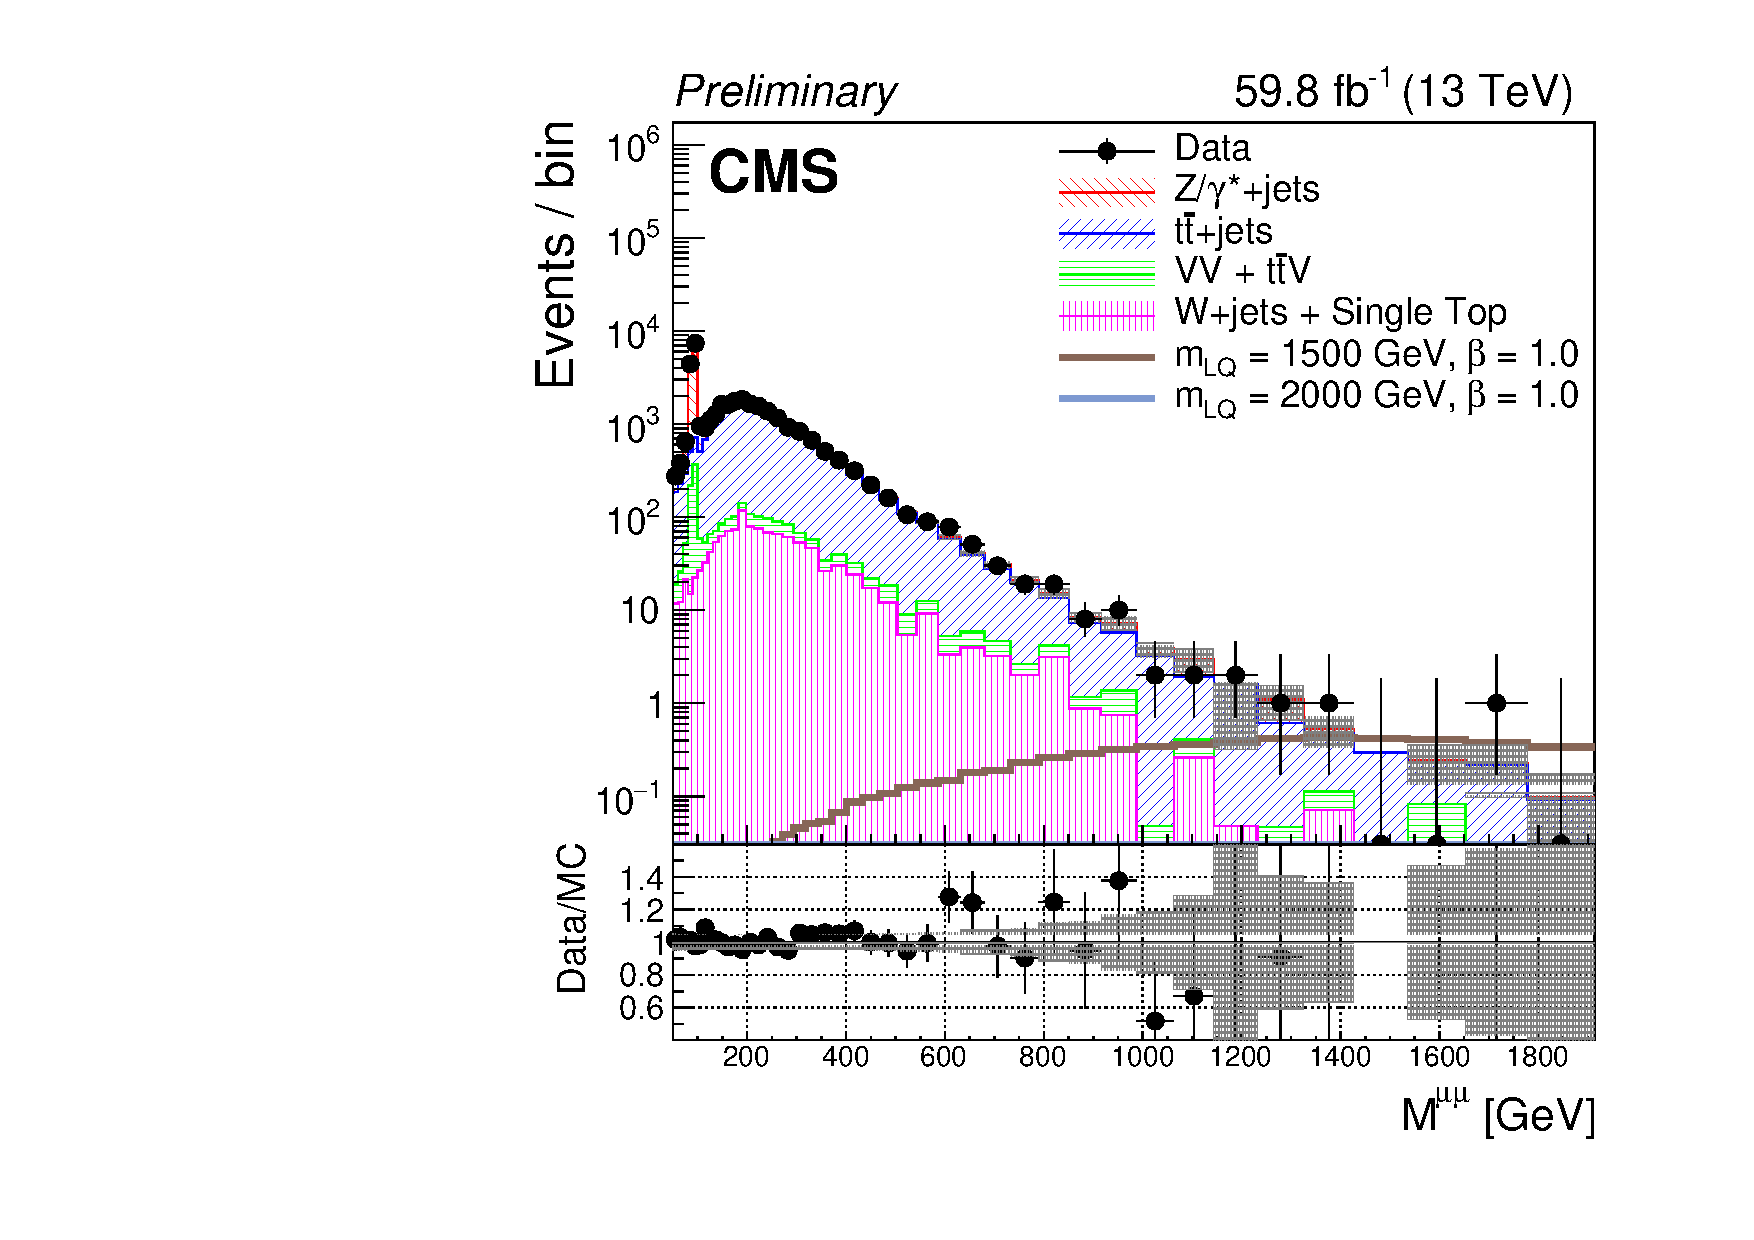
\includegraphics[width=.32\textwidth]{Images/Analysis/Results_2018_Unblinded/Plots/Preselection/BasicLQ_uujj_M_uu_standard.pdf}}
       {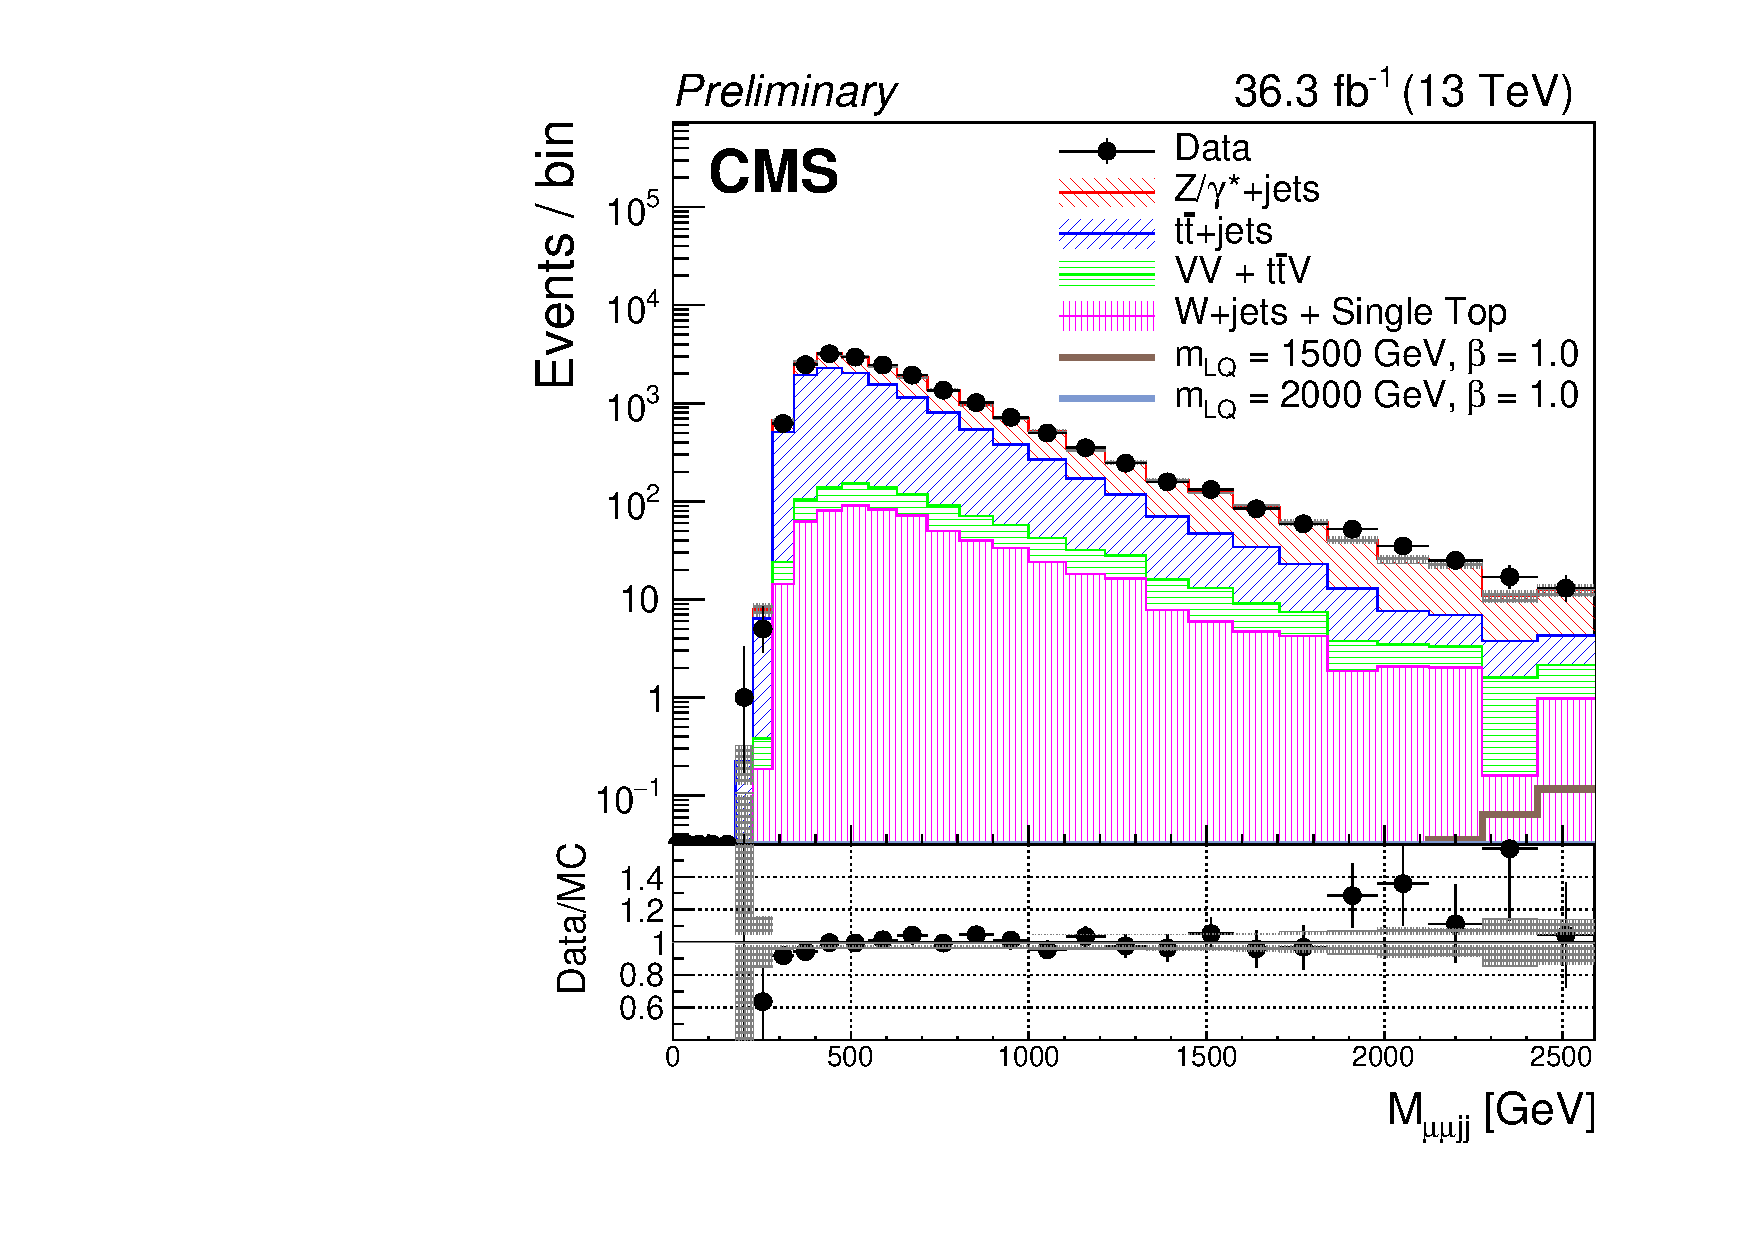
\includegraphics[width=.32\textwidth]{Images/Analysis/Results_2016_Unblinded/Plots/Preselection/BasicLQ_uujj_M_uujj_standard.pdf}}
       {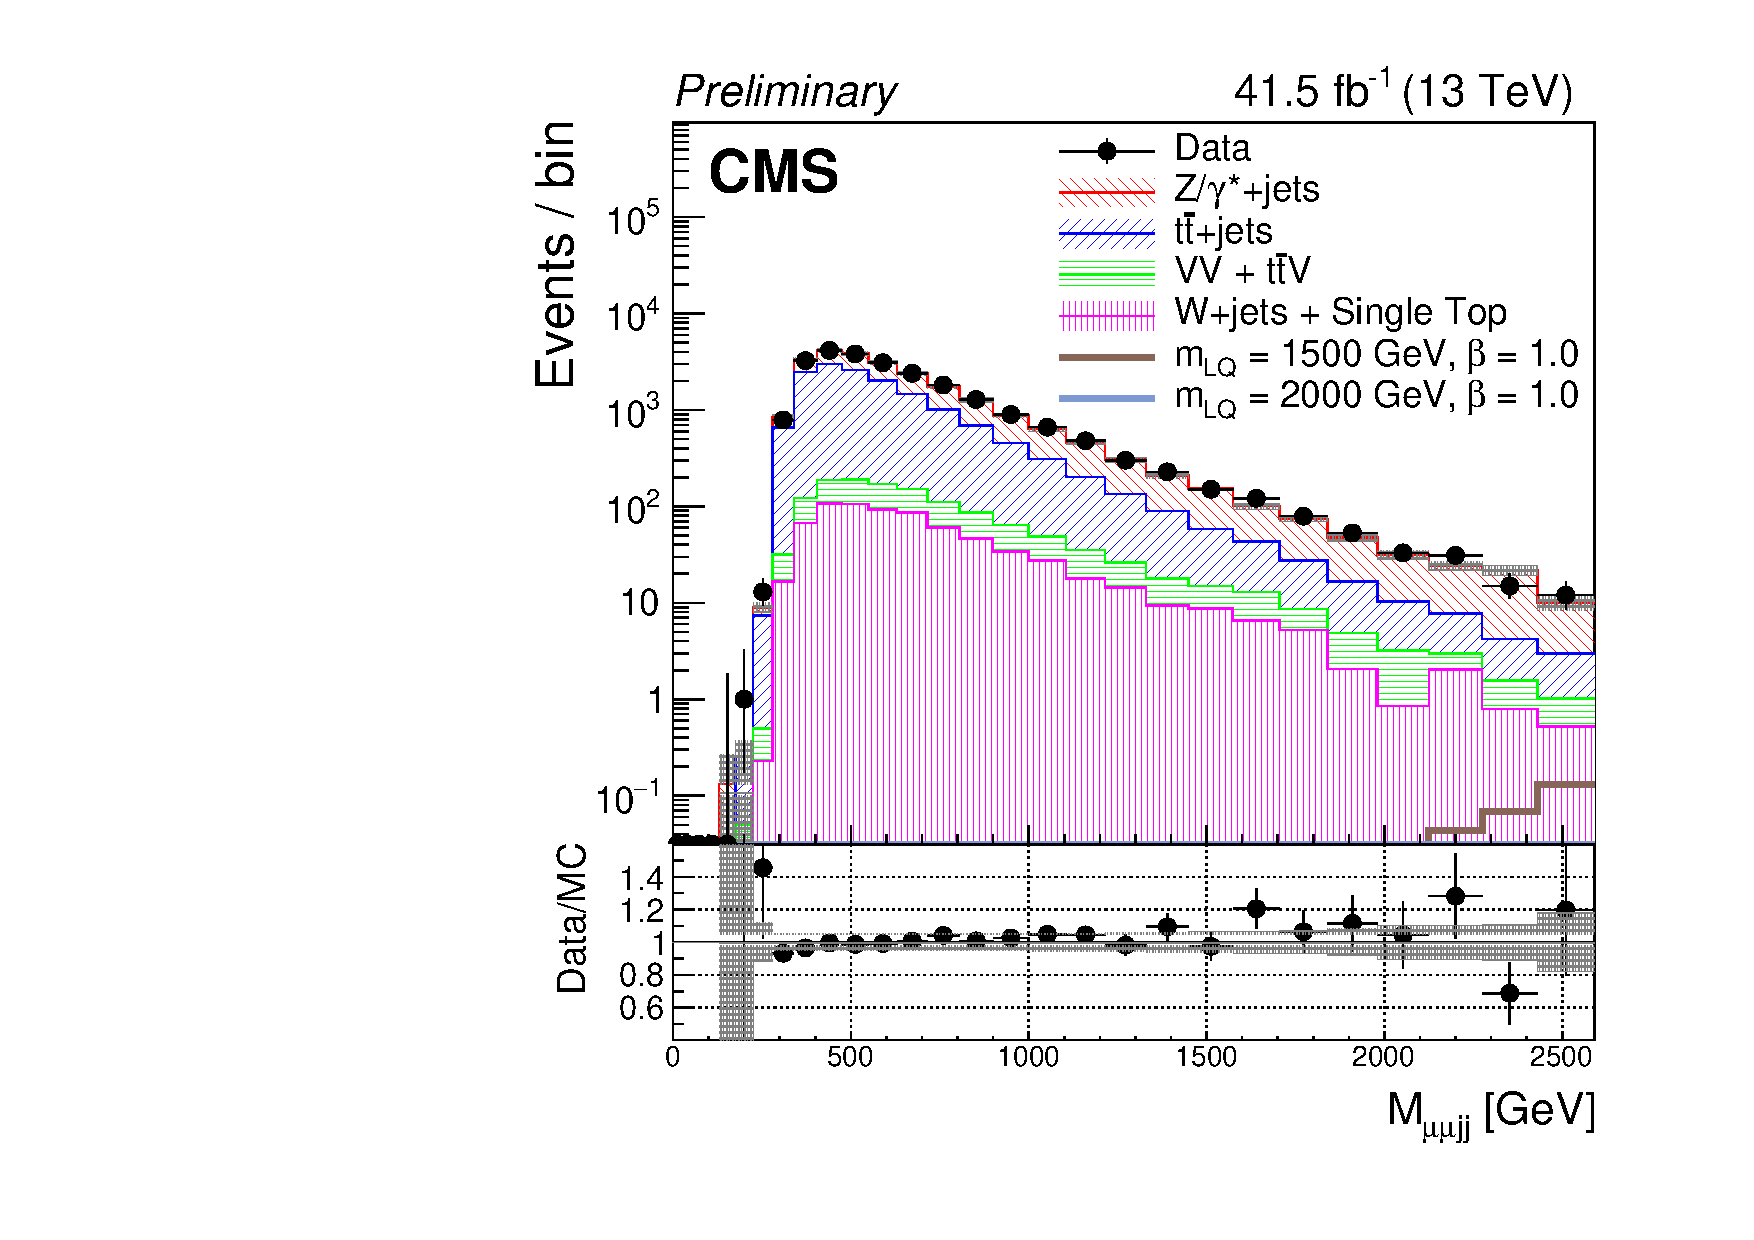
\includegraphics[width=.32\textwidth]{Images/Analysis/Results_2017_Unblinded/Plots/Preselection/BasicLQ_uujj_M_uujj_standard.pdf}}
       {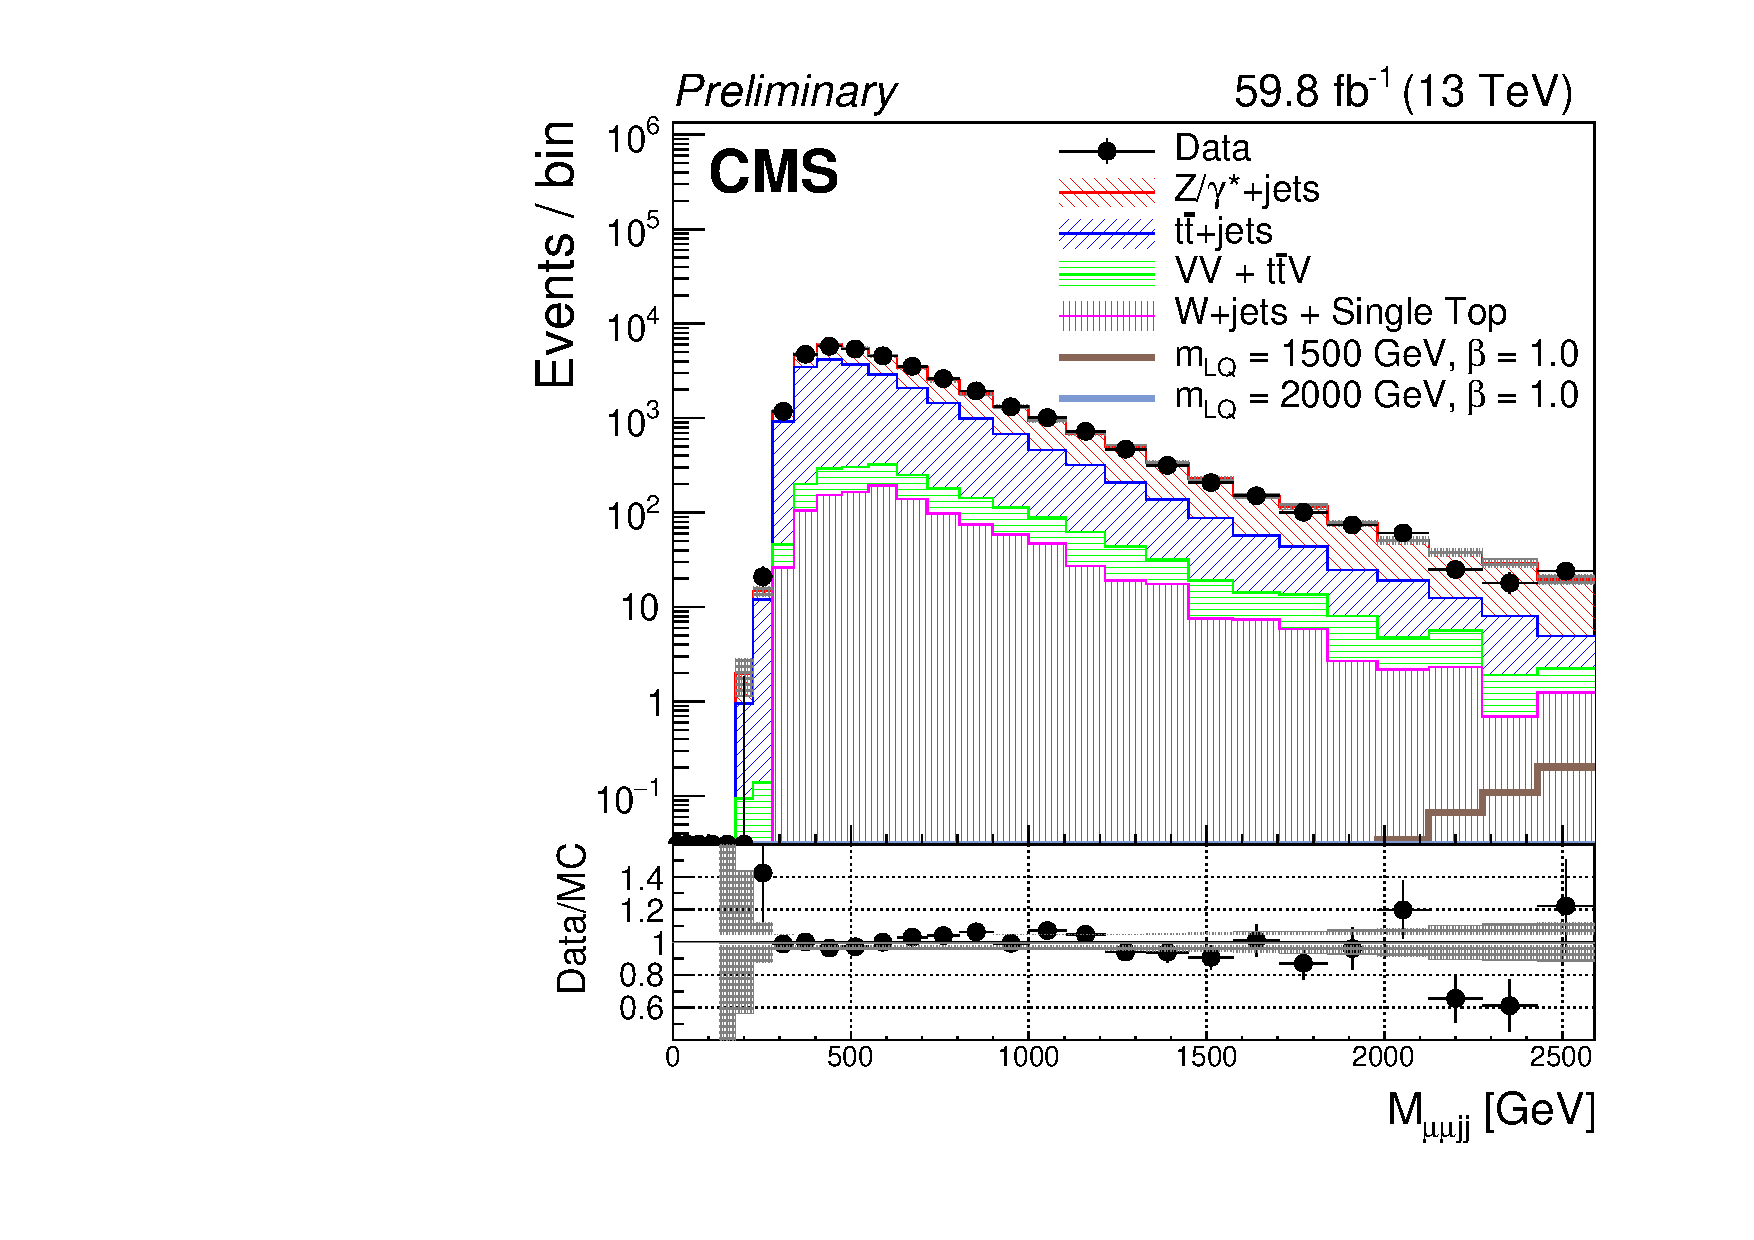
\includegraphics[width=.32\textwidth]{Images/Analysis/Results_2018_Unblinded/Plots/Preselection/BasicLQ_uujj_M_uujj_standard.pdf}}
       {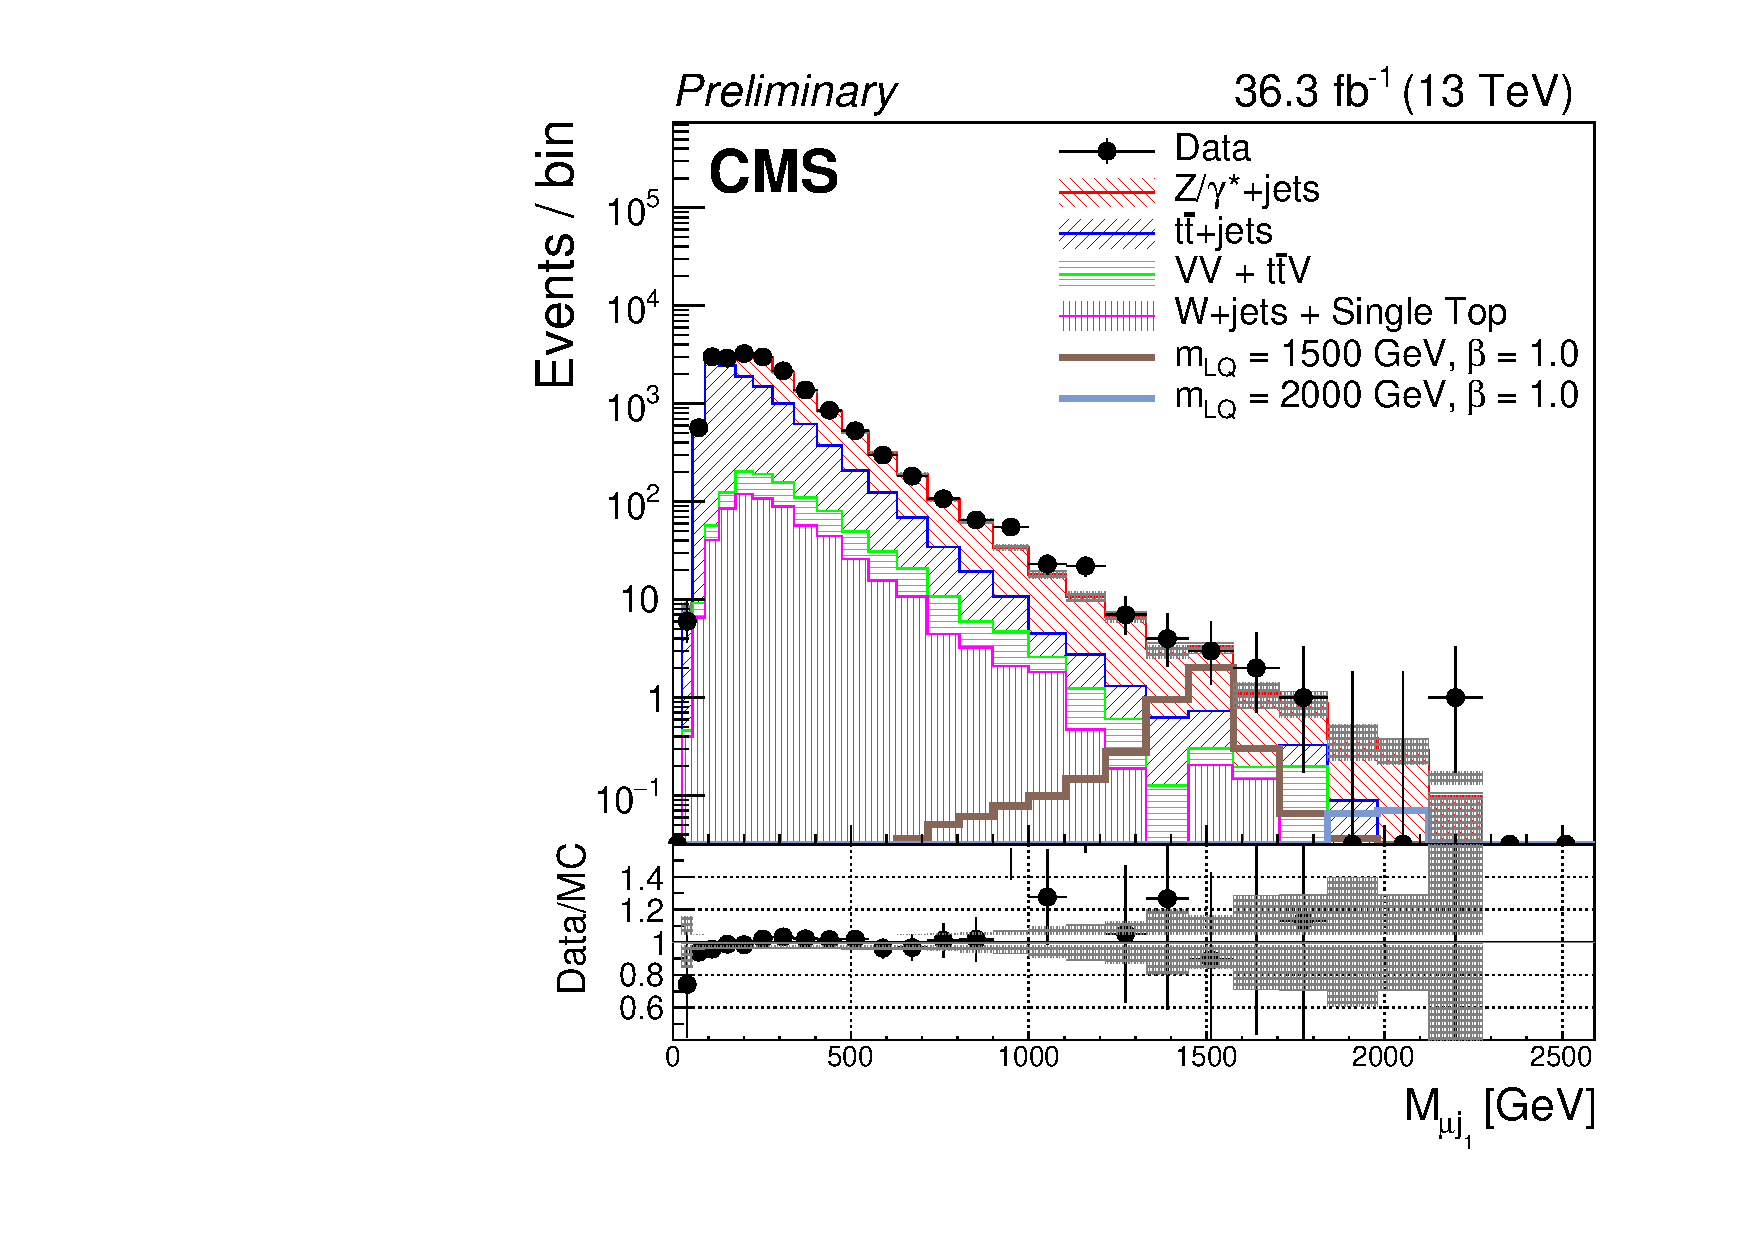
\includegraphics[width=.32\textwidth]{Images/Analysis/Results_2016_Unblinded/Plots/Preselection/BasicLQ_uujj_M_uujj1_standard.pdf}}
       {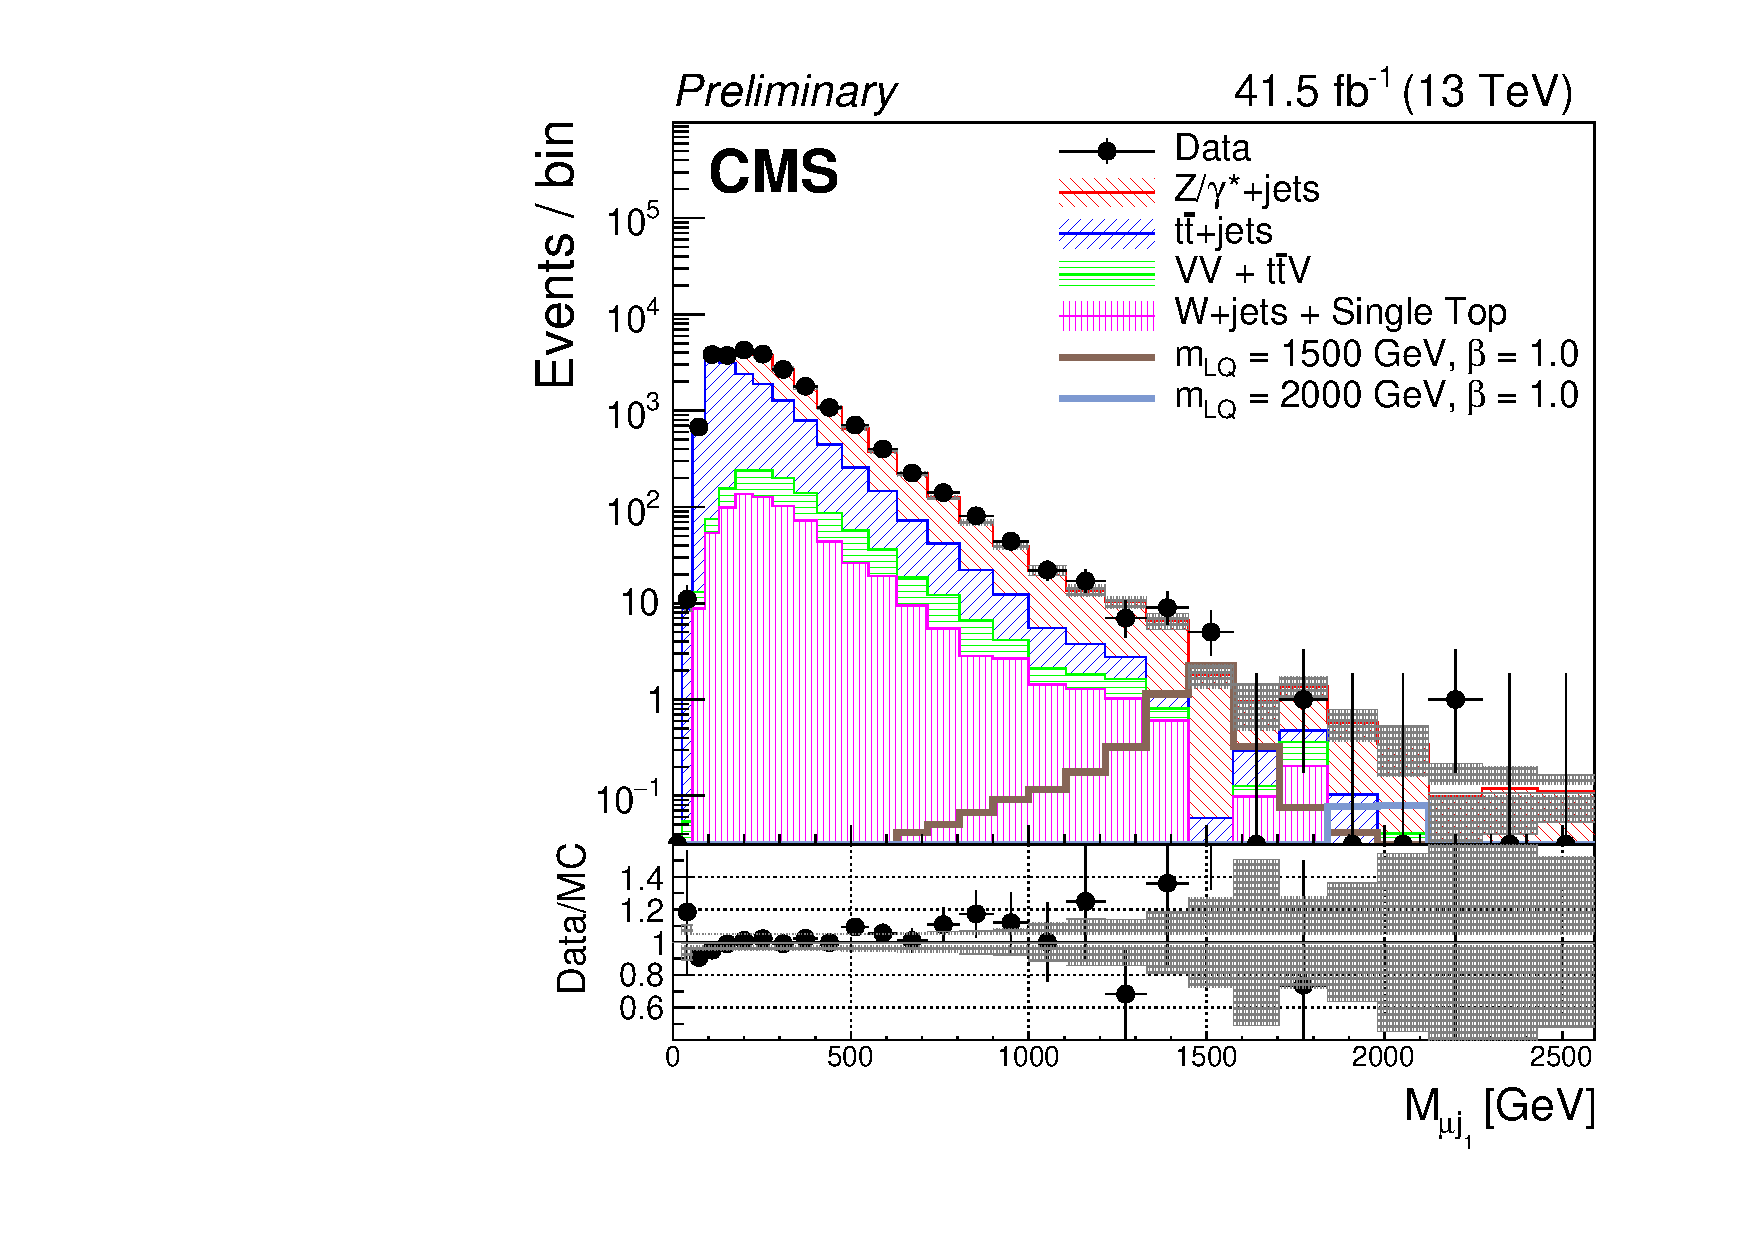
\includegraphics[width=.32\textwidth]{Images/Analysis/Results_2017_Unblinded/Plots/Preselection/BasicLQ_uujj_M_uujj1_standard.pdf}}
       {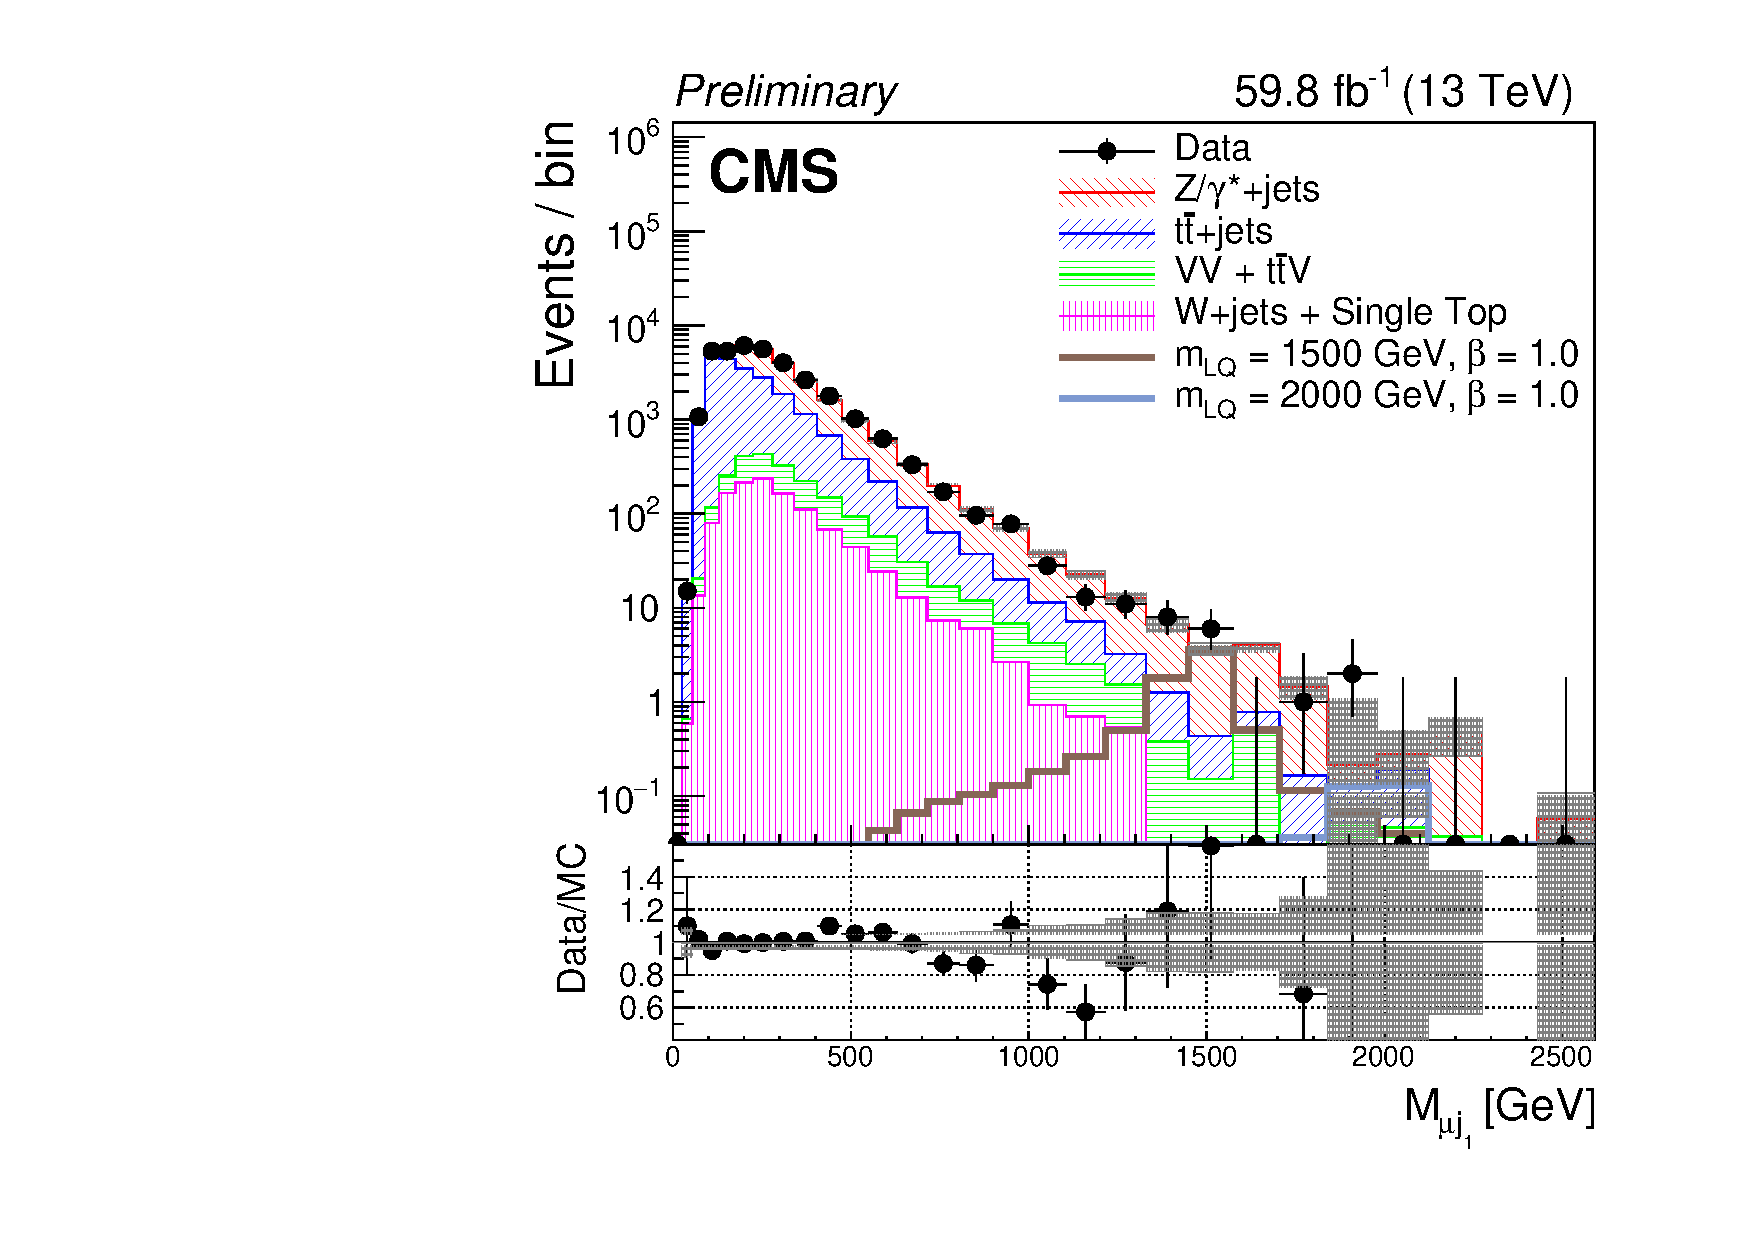
\includegraphics[width=.32\textwidth]{Images/Analysis/Results_2018_Unblinded/Plots/Preselection/BasicLQ_uujj_M_uujj1_standard.pdf}}
       {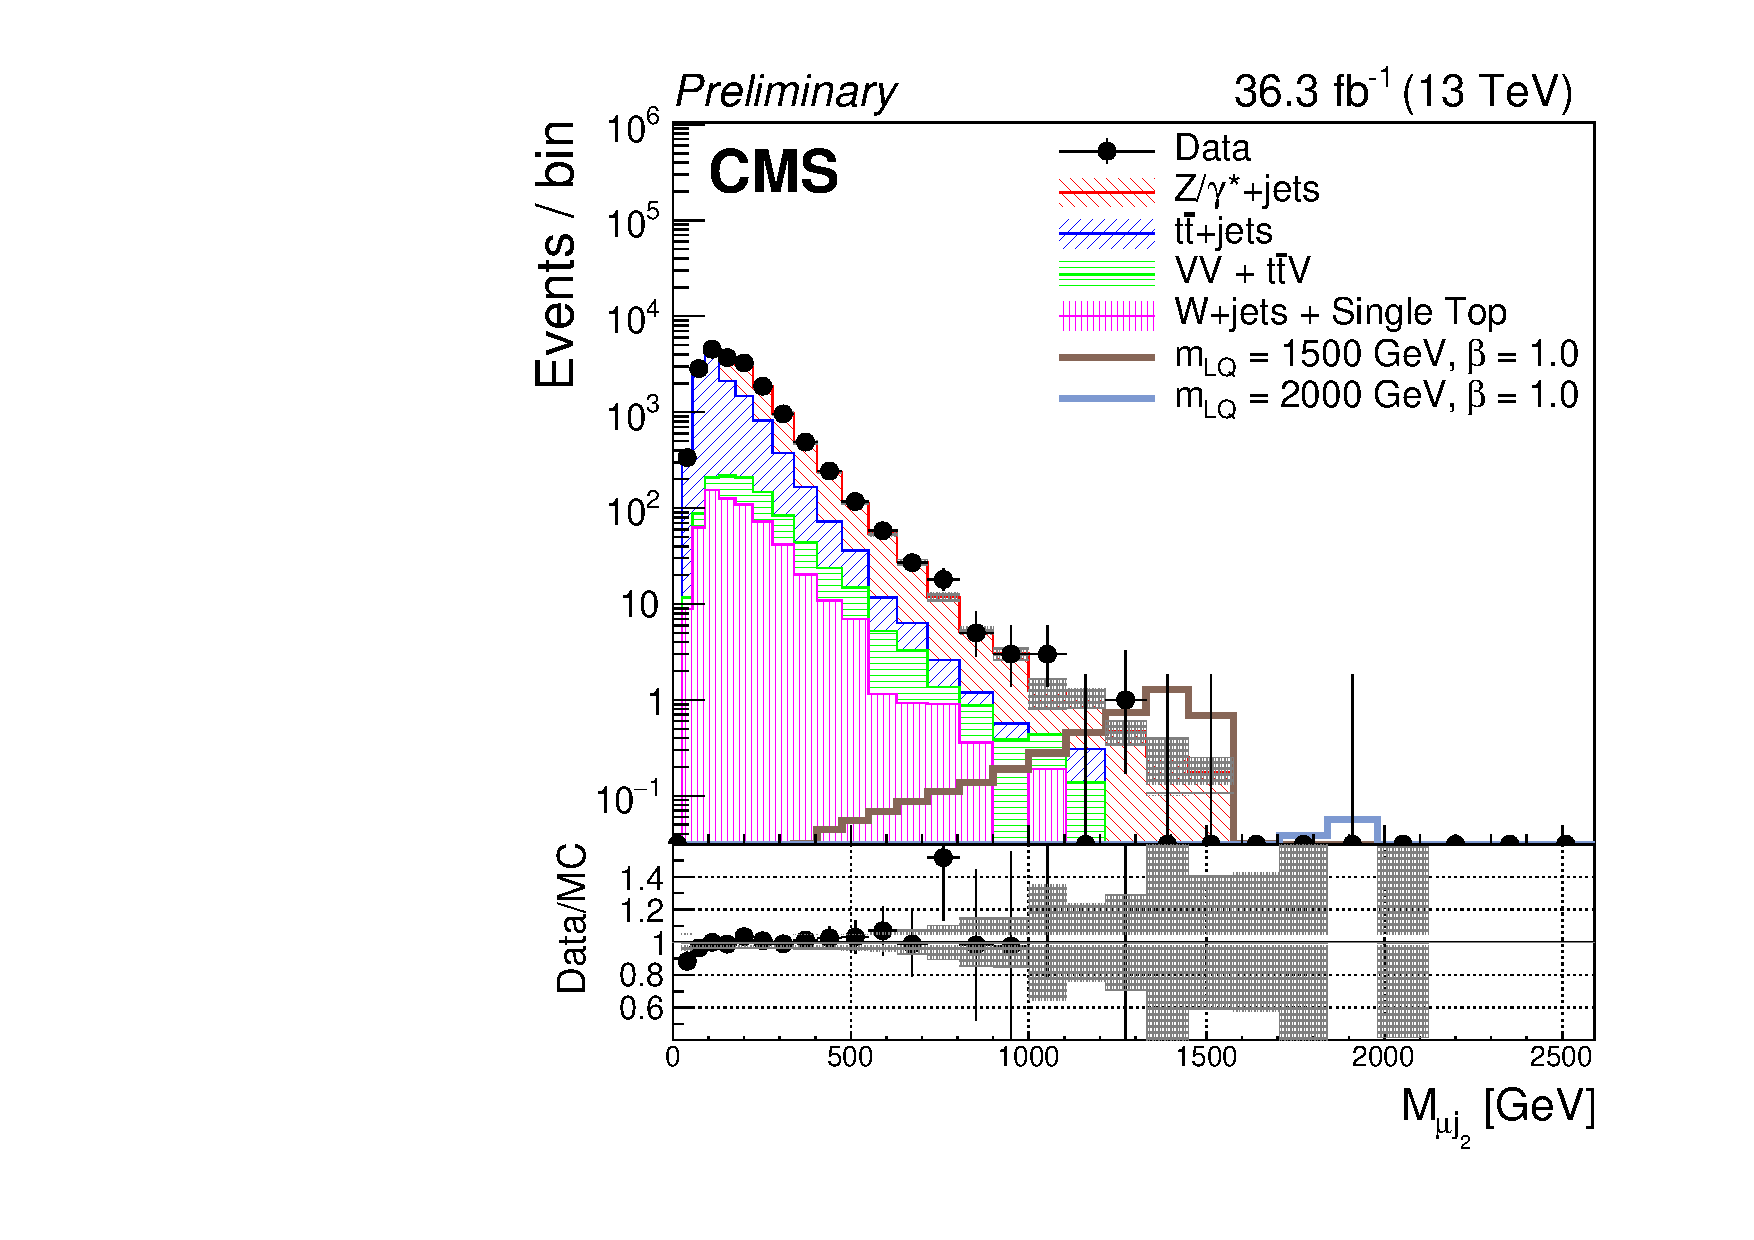
\includegraphics[width=.32\textwidth]{Images/Analysis/Results_2016_Unblinded/Plots/Preselection/BasicLQ_uujj_M_uujj2_standard.pdf}}
       {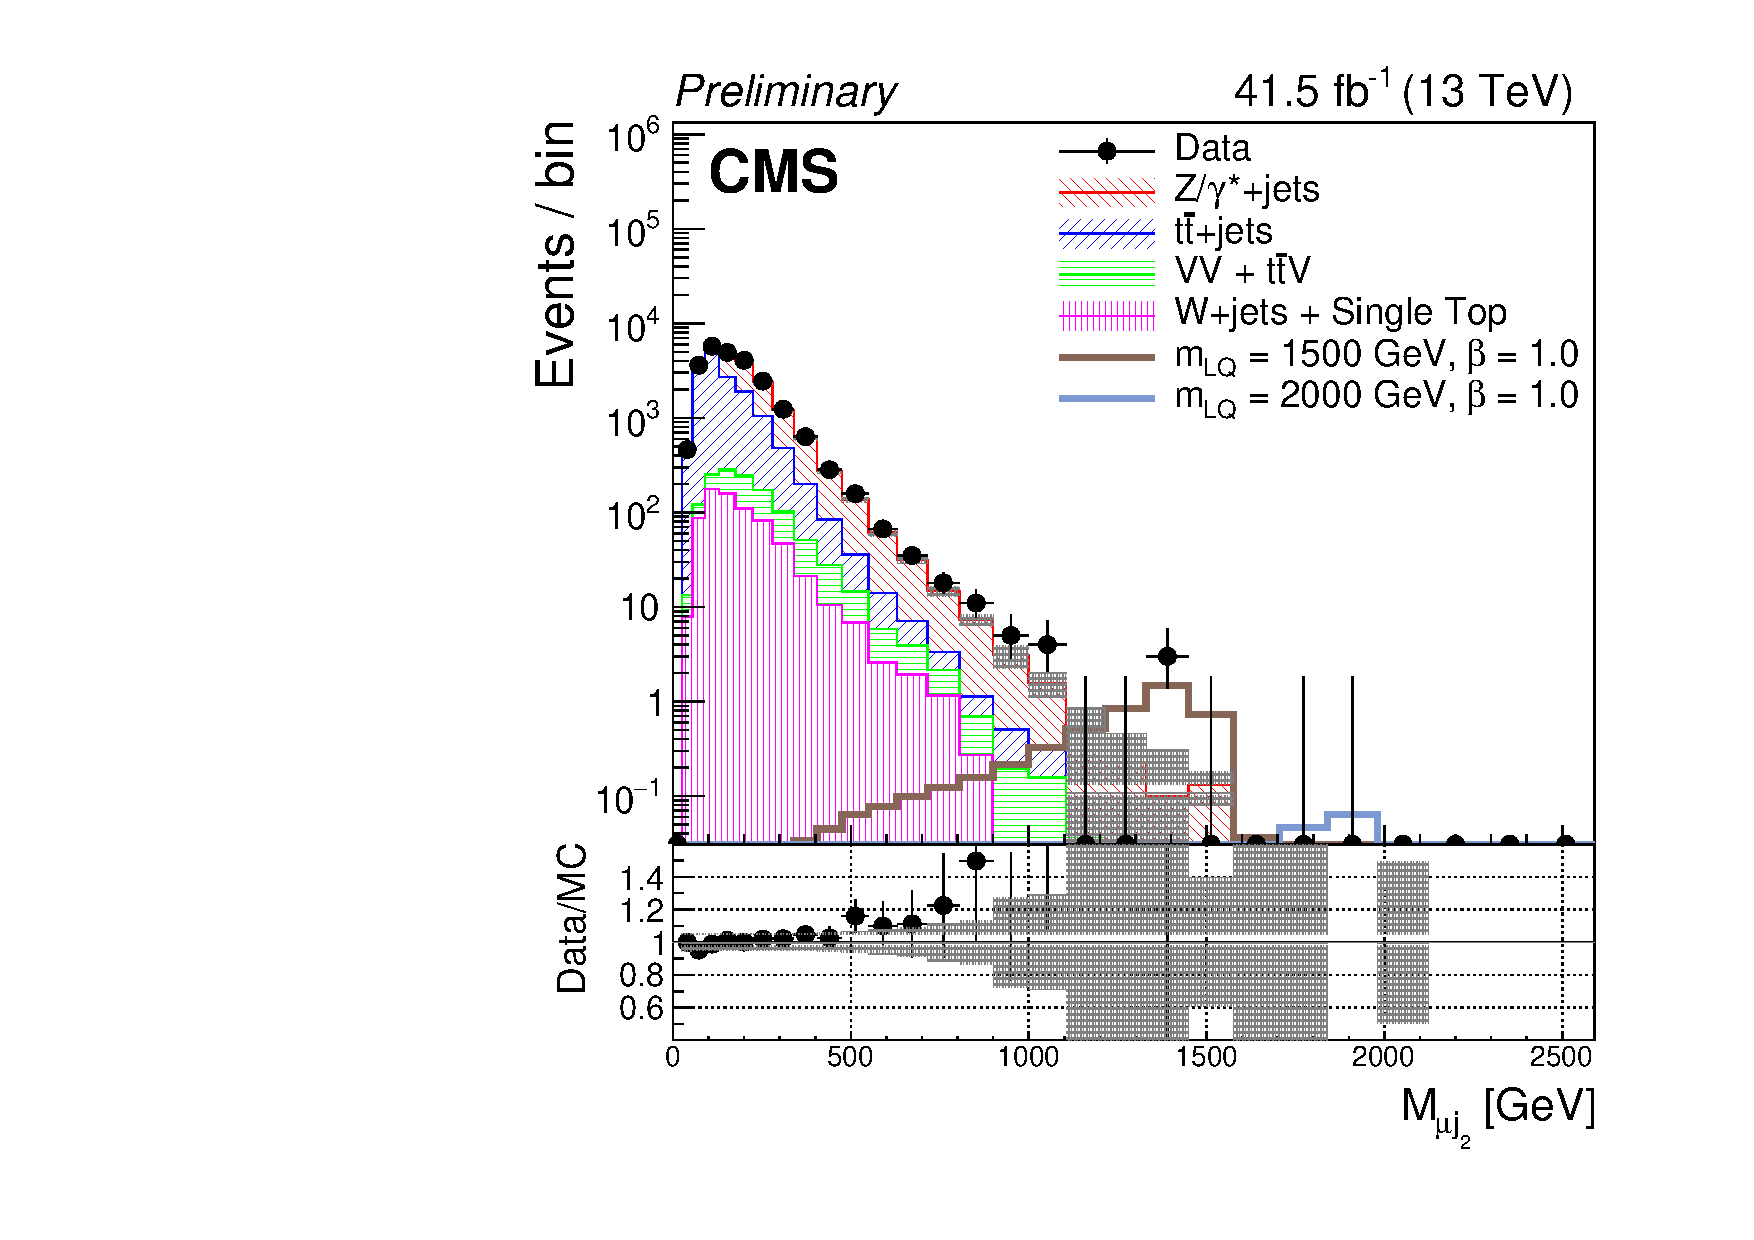
\includegraphics[width=.32\textwidth]{Images/Analysis/Results_2017_Unblinded/Plots/Preselection/BasicLQ_uujj_M_uujj2_standard.pdf}}
       {\includegraphics[width=.32\textwidth]{Images/Analysis/Results_2018_Unblinded/Plots/Preselection/BasicLQ_uujj_M_uujj2_standard.pdf}}
       \caption{A comparison between distributions of observed data and SM expectation at preselection level. Left to right: 2016, 2017, 2018 data. Top to bottom: \Muu, \Muujj, \MujOne, and \MujTwo. Error bars on observed data points represent statistical uncertainties, and systematic uncertainties on SM expectation are shown by gray hashing.}
       \label{figapp:preselmass}
\end{figure}


\begin{figure}[H]
       \centering
       {\includegraphics[width=.32\textwidth]{Images/Analysis/Results_2016_Unblinded/Plots/Preselection/BasicLQ_uujj_DeepJet_jet1_standard.pdf}}
       {\includegraphics[width=.32\textwidth]{Images/Analysis/Results_2017_Unblinded/Plots/Preselection/BasicLQ_uujj_DeepJet_jet1_standard.pdf}}
       {\includegraphics[width=.32\textwidth]{Images/Analysis/Results_2018_Unblinded/Plots/Preselection/BasicLQ_uujj_DeepJet_jet1_standard.pdf}}
       {\includegraphics[width=.32\textwidth]{Images/Analysis/Results_2016_Unblinded/Plots/Preselection/BasicLQ_uujj_DeepJet_jet2_standard.pdf}}
       {\includegraphics[width=.32\textwidth]{Images/Analysis/Results_2017_Unblinded/Plots/Preselection/BasicLQ_uujj_DeepJet_jet2_standard.pdf}}
       {\includegraphics[width=.32\textwidth]{Images/Analysis/Results_2018_Unblinded/Plots/Preselection/BasicLQ_uujj_DeepJet_jet2_standard.pdf}}
       \caption{A comparison between distributions of observed data and SM expectation at preselection level. Left to right: 2016, 2017, 2018 data. Top to bottom: DeepJet b tag score of jet 1 and DeepJet b tag score of jet 2. Error bars on observed data points represent statistical uncertainties, and systematic uncertainties on SM expectation are shown by gray hashing.}
    \label{figapp:preselbtag}
\end{figure}

% Combined plots here

\begin{figure}[H]
       \centering
       {\includegraphics[width=.49\textwidth]{Images/Analysis/Results_combined_Unblinded/Plots/Preselection/BasicLQ_uujj_GoodVertexCount_standard.pdf}}
       \caption{A comparison of the number of reconstructed vertices at preselection level in the combination of 2016, 2017, and 2018 data. Error bars shown represent statistical uncertainties, and systematic uncertainties are shown by gray hashing.}
       \label{fig:vertexCombined}
\end{figure}

\begin{figure}[H]
       \centering
       {\includegraphics[width=.49\textwidth]{Images/Analysis/Results_combined_Unblinded/Plots/Preselection/BasicLQ_uujj_Pt_muon1_standard.pdf}}
       {\includegraphics[width=.49\textwidth]{Images/Analysis/Results_combined_Unblinded/Plots/Preselection/BasicLQ_uujj_Pt_muon2_standard.pdf}}
       {\includegraphics[width=.49\textwidth]{Images/Analysis/Results_combined_Unblinded/Plots/Preselection/BasicLQ_uujj_Pt_jet1_standard.pdf}}
       {\includegraphics[width=.49\textwidth]{Images/Analysis/Results_combined_Unblinded/Plots/Preselection/BasicLQ_uujj_Pt_jet2_standard.pdf}}
       \caption{A comparison between distributions of observed data and SM expectation at preselection level in the combination of 2016, 2017, and 2018 data. Left to right, top to bottom: muon 1 \pt, muon 2 \pt, jet 1 \pt, and jet 2 \pt. Error bars on observed data points represent statistical uncertainties, and systematic uncertainties on SM expectation are shown by gray hashing.}
	\label{figa:preselptCombined}
\end{figure}

\begin{figure}[H]
       \centering
       {\includegraphics[width=0.49\textwidth]{Images/Analysis/Results_combined_Unblinded/Plots/Preselection/BasicLQ_uujj_DR_muon1jet1_standard.pdf}}
       {\includegraphics[width=0.49\textwidth]{Images/Analysis/Results_combined_Unblinded/Plots/Preselection/BasicLQ_uujj_DR_muon1jet2_standard.pdf}}
       {\includegraphics[width=0.49\textwidth]{Images/Analysis/Results_combined_Unblinded/Plots/Preselection/BasicLQ_uujj_DR_muon2jet1_standard.pdf}}
       {\includegraphics[width=0.49\textwidth]{Images/Analysis/Results_combined_Unblinded/Plots/Preselection/BasicLQ_uujj_DR_muon2jet2_standard.pdf}}
       \caption{A comparison between distributions of observed data and SM expectation at preselection level in the combination of 2016, 2017, and 2018 data. Left to right, top to bottom: \DR between muon 1 and jet 1, \DR between muon 1 and jet 2, \DR between muon 2 and jet 1, and \DR between muon 2 and jet 2. Error bars on observed data points represent statistical uncertainties, and systematic uncertainties on SM expectation are shown by gray hashing.}
       \label{fig:preseldrCombined}
\end{figure}

\begin{figure}[H]
       \centering
       {\includegraphics[width=.49\textwidth]{Images/Analysis/Results_combined_Unblinded/Plots/Preselection/BasicLQ_uujj_St_uujj_standard.pdf}}
       {\includegraphics[width=.49\textwidth]{Images/Analysis/Results_combined_Unblinded/Plots/Preselection/BasicLQ_uujj_Pt_miss_standard.pdf}}
       {\includegraphics[width=.49\textwidth]{Images/Analysis/Results_combined_Unblinded/Plots/Preselection/BasicLQ_uujj_JetCount_standard.pdf}}
       {\includegraphics[width=.49\textwidth]{Images/Analysis/Results_combined_Unblinded/Plots/Preselection/BasicLQ_uujj_MuonCount_standard.pdf}}
       \caption{A comparison between distributions of observed data and SM expectation at preselection level in the combination of 2016, 2017, and 2018 data. Left to right, top to bottom: \ST, \ptmiss, jet multiplicity, and muon multiplicity. Error bars on observed data points represent statistical uncertainties, and systematic uncertainties on SM expectation are shown by gray hashing.}
    \label{fig:preselmiscCombined}
\end{figure}

\begin{figure}[H]
       \centering
       {\includegraphics[width=.49\textwidth]{Images/Analysis/Results_combined_Unblinded/Plots/Preselection/BasicLQ_uujj_M_uu_standard.pdf}}
       {\includegraphics[width=.49\textwidth]{Images/Analysis/Results_combined_Unblinded/Plots/Preselection/BasicLQ_uujj_M_uujj_standard.pdf}}
       {\includegraphics[width=.49\textwidth]{Images/Analysis/Results_combined_Unblinded/Plots/Preselection/BasicLQ_uujj_M_uujj1_standard.pdf}}
       {\includegraphics[width=.49\textwidth]{Images/Analysis/Results_combined_Unblinded/Plots/Preselection/BasicLQ_uujj_M_uujj2_standard.pdf}}
       \caption{A comparison between distributions of observed data and SM expectation at preselection level in the combination of 2016, 2017, and 2018 data. Left to right, top to bottom: \Muu, \Muujj, \MujOne, and \MujTwo. Error bars on observed data points represent statistical uncertainties, and systematic uncertainties on SM expectation are shown by gray hashing.}
       \label{fig:preselmassCombined}
\end{figure}


\begin{figure}[H]
       \centering
       {\includegraphics[width=.49\textwidth]{Images/Analysis/Results_combined_Unblinded/Plots/Preselection/BasicLQ_uujj_DeepJet_jet1_standard.pdf}}
       {\includegraphics[width=.49\textwidth]{Images/Analysis/Results_combined_Unblinded/Plots/Preselection/BasicLQ_uujj_DeepJet_jet2_standard.pdf}}
       \caption{A comparison between distributions of observed data and SM expectation at preselection level in the combination of 2016, 2017, and 2018 data. Left to Right: DeepJet b tag score of jet 1 and DeepJet b tag score of jet 2. Error bars on observed data points represent statistical uncertainties, and systematic uncertainties on SM expectation are shown by gray hashing.}
    \label{fig:preselbtagCombined}
\end{figure}
